\begin{frame}{Grobgliederung}

\tableofcontents

\end{frame}

\section{Vorwort}\label{vorwort}

\begin{frame}{Hinweise}

\begin{itemize}
\item
  Diese Folien vermitteln \emph{nicht} den Stoff. Sie visualisieren nur
  einige zentrale Ideen.
\item
  Der Stoff wird vom
  \href{https://sebastiansauer.github.io/Praxis_der_Datenanalyse/}{Skript}
  vermittelt. Nutzen Sie das Skript zum eigentlichen Arbeiten.
\end{itemize}

\end{frame}

\section{Organisatorisches}\label{organisatorisches}

\begin{frame}{Modulziele}

Die Studierenden können nach erfolgreichem Abschluss des Moduls:

\begin{itemize}
\tightlist
\item
  den Ablauf eines Projekts aus der Datenanalyse in wesentlichen
  Schritten nachvollziehen,
\item
  Daten aufbereiten und ansprechend visualisieren,
\item
  Inferenzstatistik anwenden und kritisch hinterfragen,
\item
  klassische Vorhersagemethoden (Regression) anwenden,
\item
  moderne Methoden der angewandten Datenanalyse anwenden (z.B.
  Textmining),
\item
  betriebswirtschaftliche Fragestellungen mittels datengetriebener
  Vorhersagemodellen beantworten.
\end{itemize}

\end{frame}

\begin{frame}{Themen pro Termin (insgesamt 44UE Lehre)}

\footnotesize

\begin{longtable}[]{@{}rl@{}}
\toprule
Termin & Thema / Kapitel\tabularnewline
\midrule
\endhead
1 & Organisatorisches\tabularnewline
1 & Einführung\tabularnewline
1 & Rahmen\tabularnewline
1 & Daten einlesen\tabularnewline
2 & Datenjudo\tabularnewline
3 & Daten visualisieren\tabularnewline
4 & Fallstudie (z.B. zu `movies')\tabularnewline
5 & Daten modellieren\tabularnewline
5 & Der p-Wert\tabularnewline
6 & Lineare Regression - metrisch\tabularnewline
7 & Lineare Regression - kategorial\tabularnewline
8 & Fallstudie (z.B. zu `titanic' und `affairs')\tabularnewline
9 & Vertiefung 1: Textmining oder Clusteranalyse\tabularnewline
10 & Vertiefung 2: Dimensionsreduktion\tabularnewline
11 & Wiederholung\tabularnewline
\bottomrule
\end{longtable}

\end{frame}

\begin{frame}{Prüfung - Allgemeine Hinweise}

\begin{itemize}
\tightlist
\item
  Die Prüfung besteht aus zwei Teilen

  \begin{itemize}
  \tightlist
  \item
    einer Klausur (50\% der Teilnote)
  \item
    einer Datenanalyse (50\% der Teilnote).
  \end{itemize}
\end{itemize}

\emph{Prüfungsrelevant} ist der gesamte Stoff aus dem Skript und dem
Unterricht mit
\href{https://sebastiansauer.github.io/Praxis_der_Datenanalyse/organisatorisches.html\#prufung}{einigen
Ausnahmen}

Alle Hinweise zur Prüfung gelten nur insoweit nicht anders vom Dozenten
festgelegt.

\end{frame}

\begin{frame}{Klausur und Datenanalyse}

\begin{block}{Klausur}

\begin{itemize}
\tightlist
\item
  Hinweise zur Klausur finden Sie
  \href{https://sebastiansauer.github.io/Praxis_der_Datenanalyse/organisatorisches.html\#klausur}{hier}
\item
  Im Skript finden Sie eine
  \href{https://sebastiansauer.github.io/Praxis_der_Datenanalyse/probeklausur.html}{Probeklausur}.
\item
  Lernaufgaben finden sich im Skript am Ende jedes Kapitels.
\end{itemize}

\end{block}

\begin{block}{Datenanalyse}

\begin{itemize}
\tightlist
\item
  Hinweise zur Datenanalyse finden Sie
  \href{https://sebastiansauer.github.io/Praxis_der_Datenanalyse/organisatorisches.html\#klausur}{hier}.
\item
  Die Datenanalyse wird (in fast jeder Stunde) praktisch eingeübt.
\item
  Beispiele für gute Datenanalysen von Studierenden finden Sie
  \href{https://sebastiansauer.github.io/Praxis_der_Datenanalyse/organisatorisches.html\#klausur}{hier}
  (im OC).
\end{itemize}

\end{block}

\end{frame}

\section{Rahmen}\label{rahmen}

\begin{frame}{Lernziele}

\begin{itemize}
\tightlist
\item
  Einen Überblick über die fünf wesentliche Schritte der Datenanalyse
  gewinnen.
\item
  R und RStudio installieren können.
\item
  Einige häufige technische Probleme zu lösen wissen.
\item
  R-Pakete installieren können.
\item
  Einige grundlegende R-Funktionalitäten verstehen.
\item
  Auf die Frage ``Was ist Statistik?'' eine Antwort geben können.
\end{itemize}

\end{frame}

\begin{frame}{Prozess der Datenanalyse - Überblick über das Modul}

\begin{figure}

{\centering 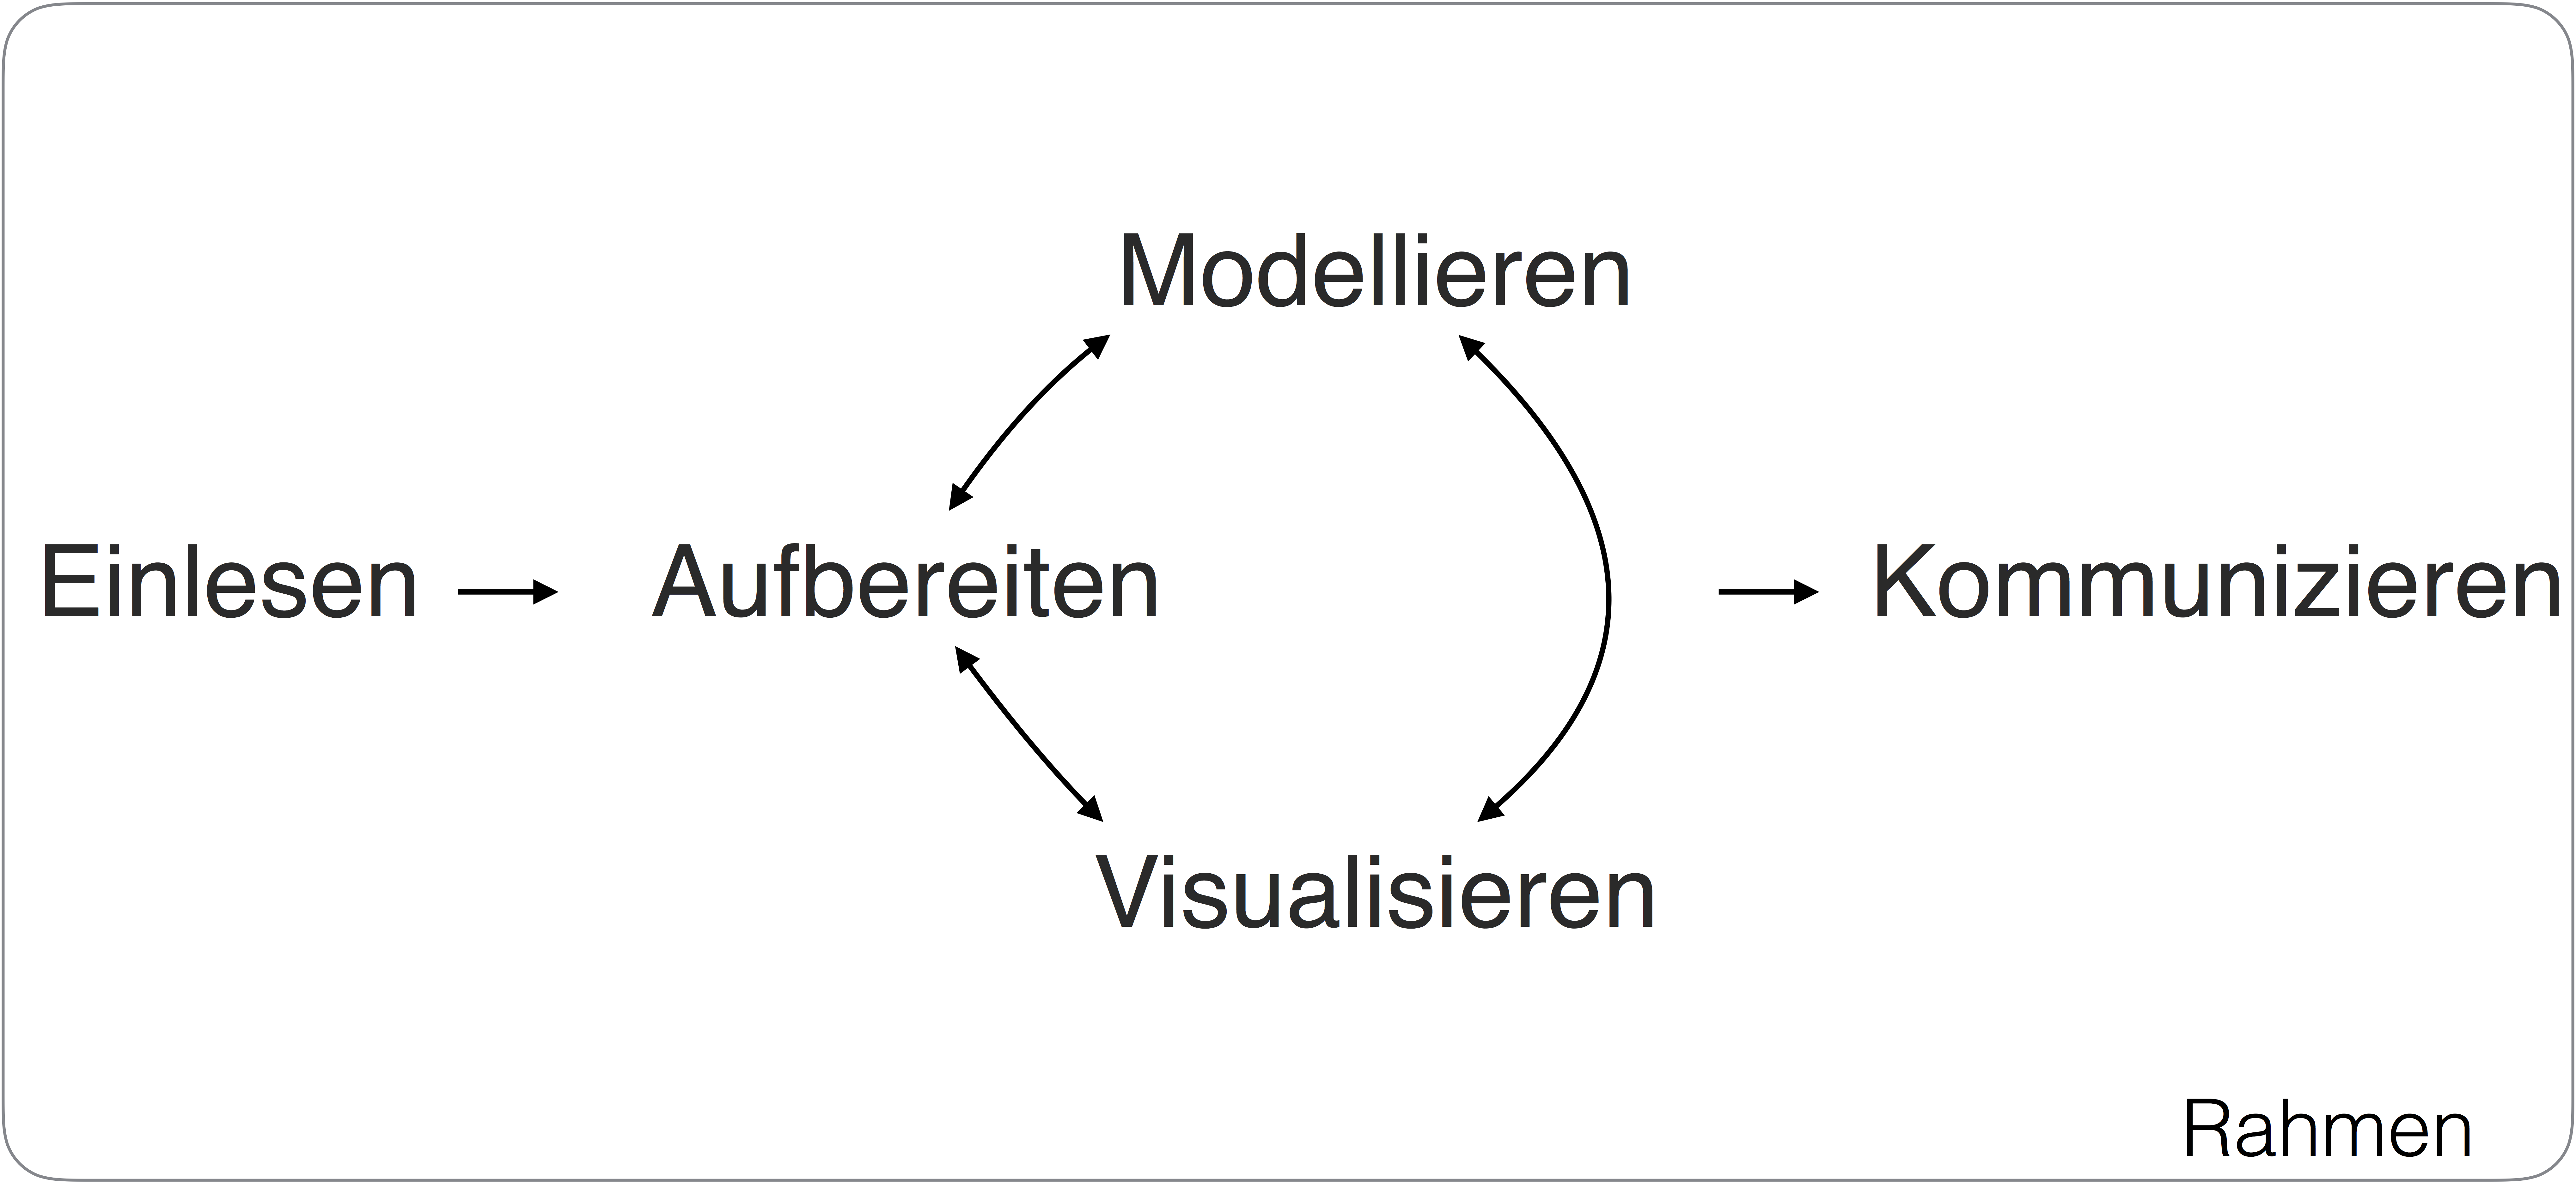
\includegraphics[width=0.8\linewidth]{../images/Rahmen/Prozess_Datenanalyse} 

}

\caption{Der Prozess der Datenanalyse}\label{fig:fig-prozess}
\end{figure}

\end{frame}

\begin{frame}{R und RStudio installieren}


\includegraphics[width=0.10000\textwidth]{../images/Rahmen/Rlogo.png}

\includegraphics[width=0.10000\textwidth]{../images/Rahmen/rstudiologo.png}

\begin{figure}

{\centering 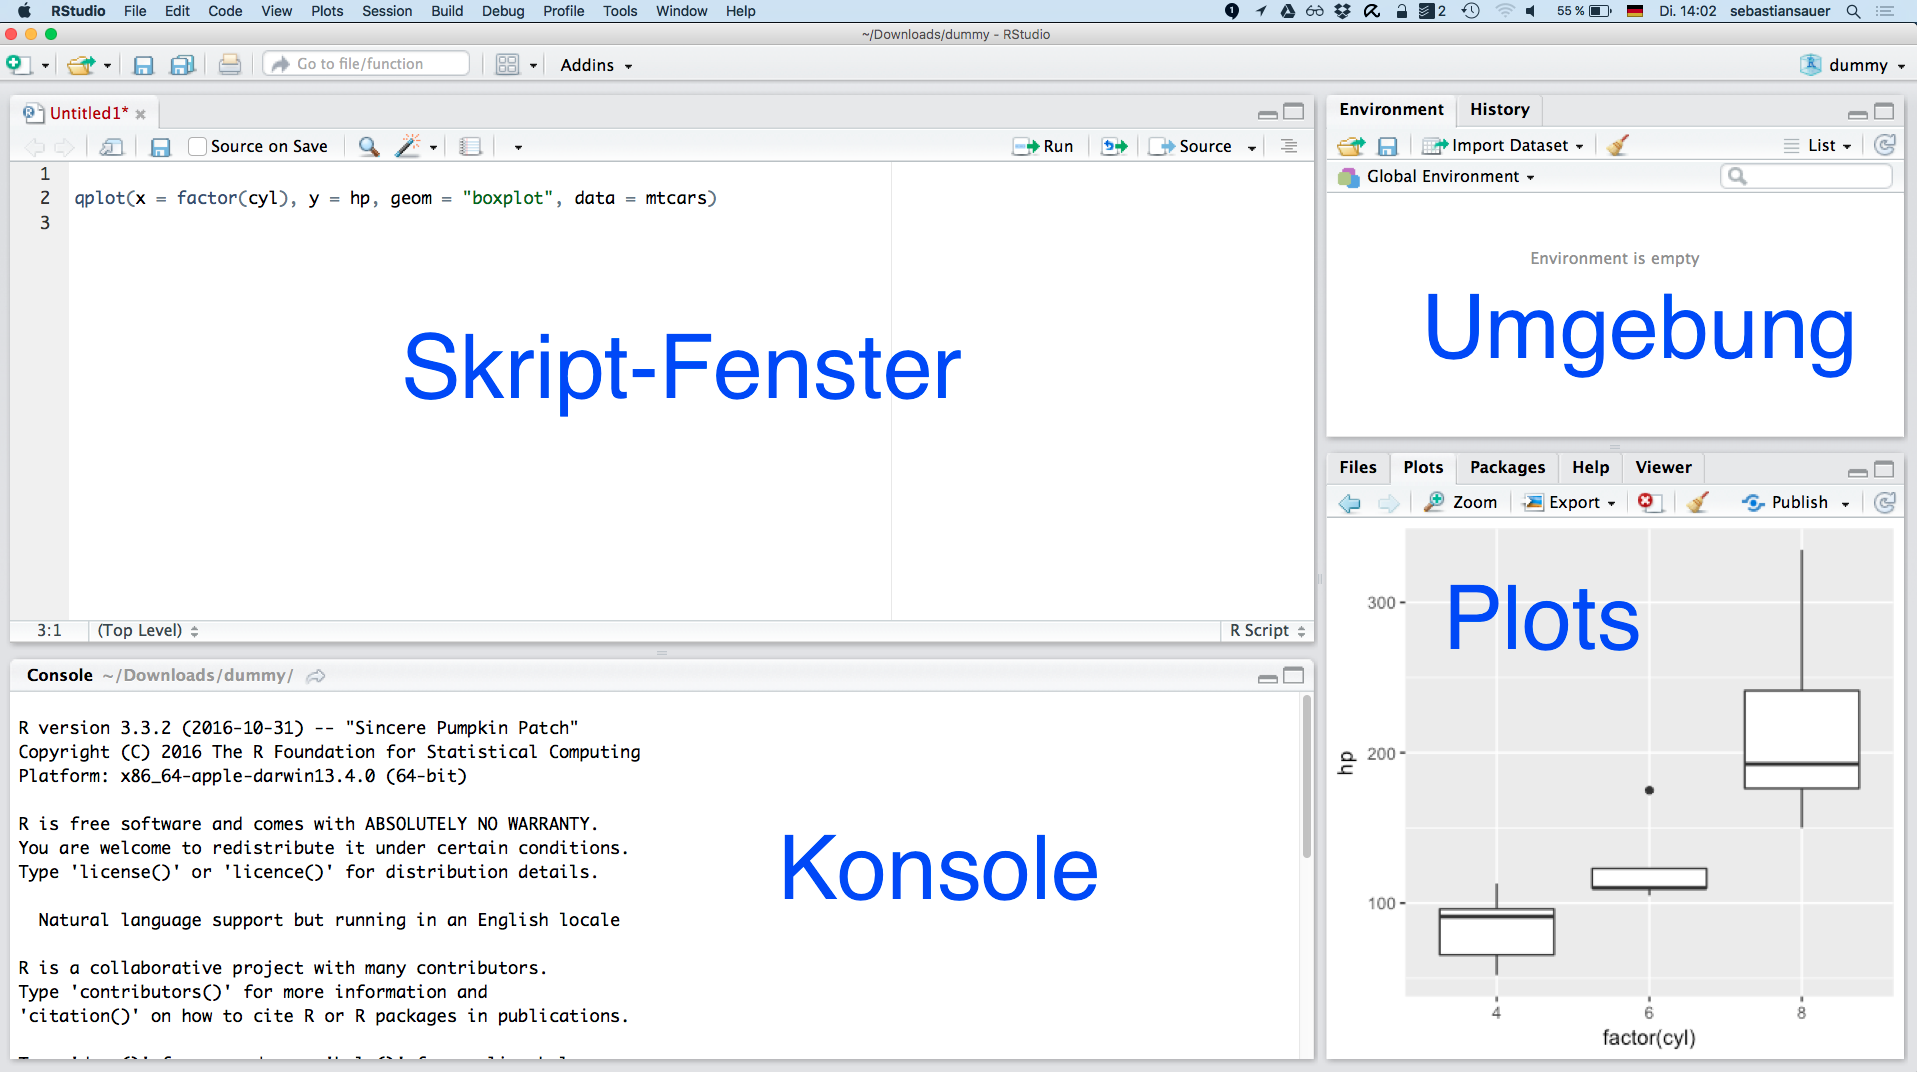
\includegraphics[width=0.5\linewidth]{../images/Rahmen/RStudio-Screenshot} 

}

\caption{RStudio}\label{fig:unnamed-chunk-1}
\end{figure}

\end{frame}

\begin{frame}{Sonstiges Material für dieses Skript}

Bitte laden Sie sich diesen Ordner
\href{https://github.com/sebastiansauer/Praxis_der_Datenanalyse/tree/gh-pages}{Github-Repositorium}
herunter. Dazu klicken Sie auf den grünen Button ``Clone or Download'',
wählen Sie dann ``Download Zip''. Daraufhin wird dieser Ordner
heruntergeladen.

\end{frame}

\begin{frame}[fragile]{Hilfe! R!}

Beliebte Fehler beim Installieren von Paketen:

\begin{verbatim}
- install.packages(dplyr) 

- install.packages("dliar")

- install.packages("derpyler") 

- install.packages("dplyr")  # dependencies vergessen 

- Keine Internet-Verbindung 

- library(dplyr)  # ohne vorher zu installieren
\end{verbatim}

\end{frame}

\begin{frame}{Pakete installieren leichtgemacht}

\begin{figure}

{\centering 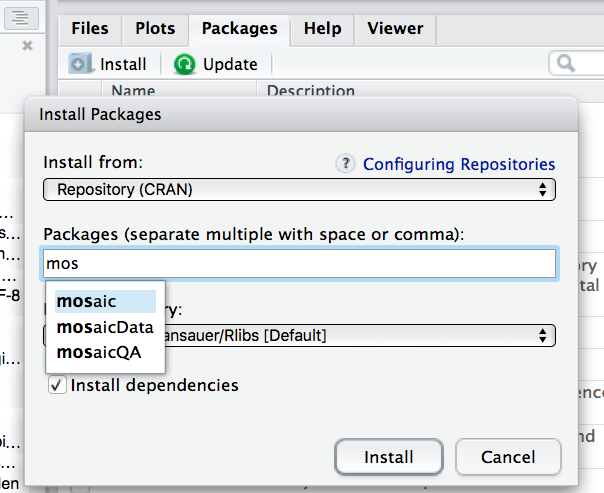
\includegraphics[width=0.5\linewidth]{../images/Rahmen/install_packages} 

}

\caption{So installiert man Pakete in RStudio}\label{fig:fig-install-packages}
\end{figure}

\end{frame}

\begin{frame}[fragile]{Datensätze}

Alle Datensätze liegen im Ordner \texttt{data/}, den Sie vom
\href{https://github.com/sebastiansauer/Praxis_der_Datenanalyse}{Github-Repositorium}
herunterladen können.

\end{frame}

\begin{frame}{Was ist Statistik?}

\emph{Eine} Antwort dazu ist, dass Statistik die Wissenschaft von
Sammlung, Analyse, Interpretation und Kommunikation von Daten ist
mithilfe mathematischer Verfahren ist und zur Entscheidungshilfe
beitragen soll.

\begin{figure}

{\centering 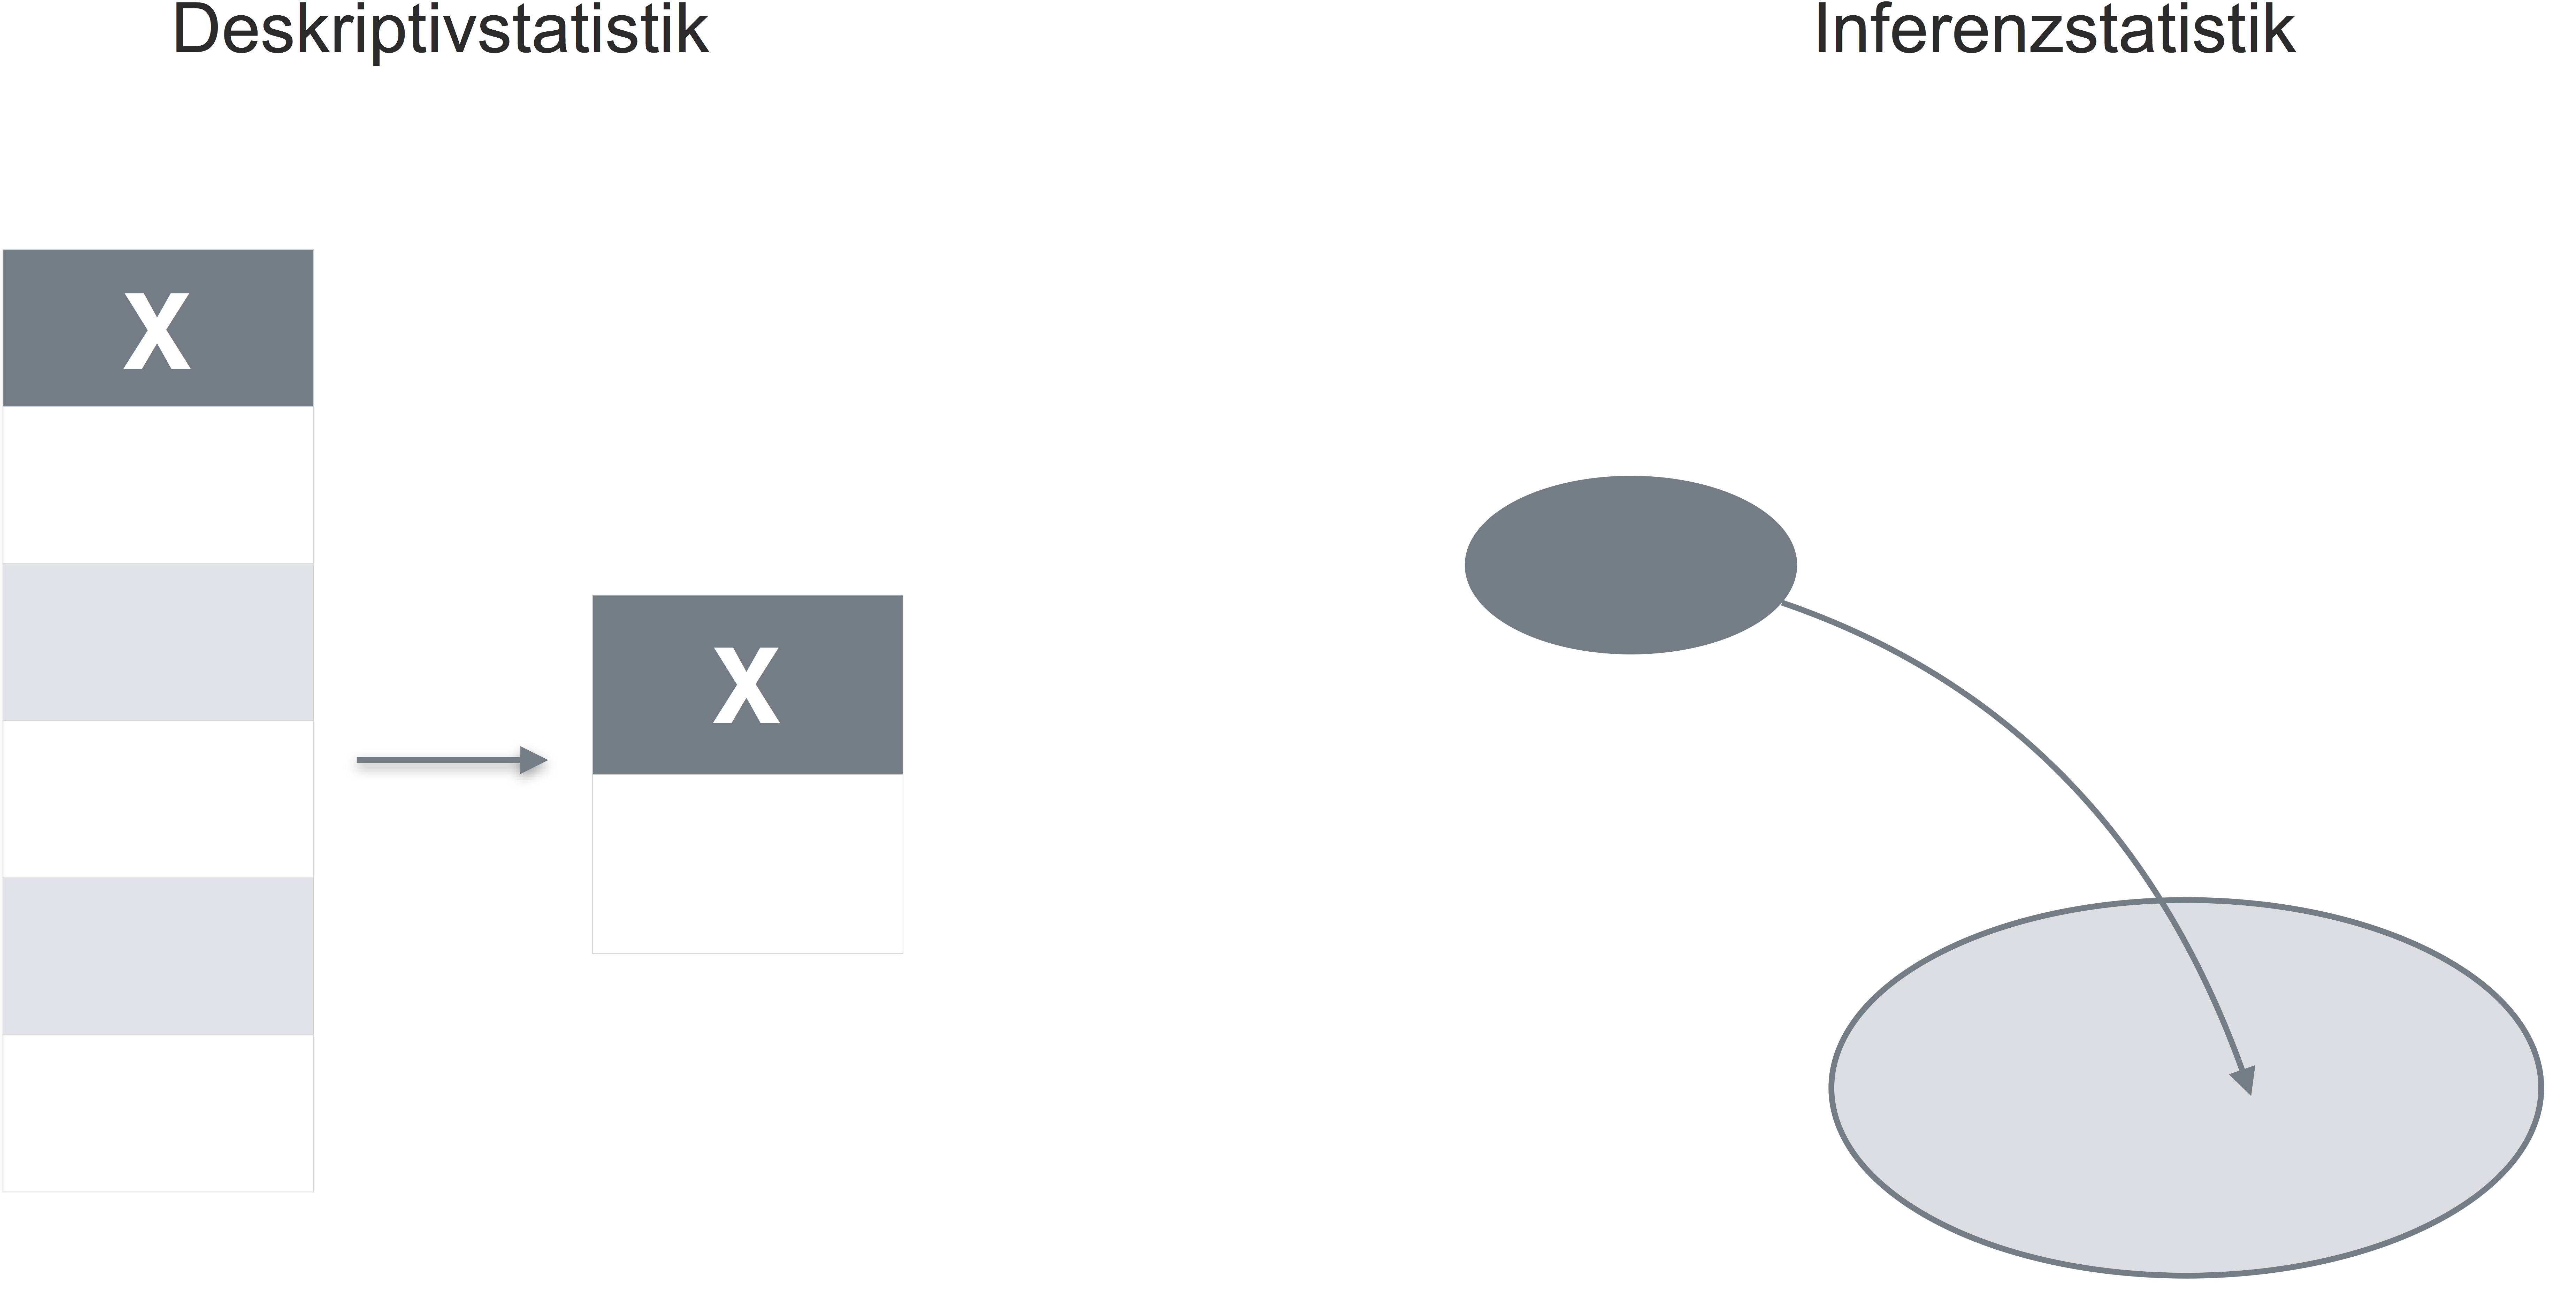
\includegraphics[width=0.8\linewidth]{../images/Rahmen/desk_vs_inf-crop} 

}

\caption{Sinnbild für die Deskriptiv- und die Inferenzstatistik}\label{fig:desk-vs-inf}
\end{figure}

\end{frame}

\begin{frame}[fragile]{Abduktion als klassische Denkfigur in der
Statistik}

\begin{verbatim}
Prämisse 1: Wenn Modell M wahr ist,   
dann sollten die Daten das Muster D aufweisen.
Prämisse 2: Die Daten weisen das Muster D auf.
---
Konklusion: Daher muss das Modell M wahr sein.
\end{verbatim}

Die Konklusion ist \emph{nicht} zwangsläufig richtig.

\end{frame}

\section{Daten einlesen}\label{tidy}

\begin{frame}{Lernziele}

\begin{itemize}
\tightlist
\item
  Wissen, was eine CSV-Datei ist.
\item
  Wissen, was UTF-8 bedeutet.
\item
  Erläutern können, was R unter dem ``working directory'' versteht.
\item
  Erkennen können, ob eine Tabelle in Normalform vorliegt.
\item
  Daten aus R hinauskriegen (exportieren).
\end{itemize}

Dieses Kapitel beantwortet eine Frage: ``Wie kriege ich Daten in
vernünftiger Form in R hinein?''.

\end{frame}

\begin{frame}{Prozess der Datenanalyse -- Einlesen}

\begin{figure}

{\centering 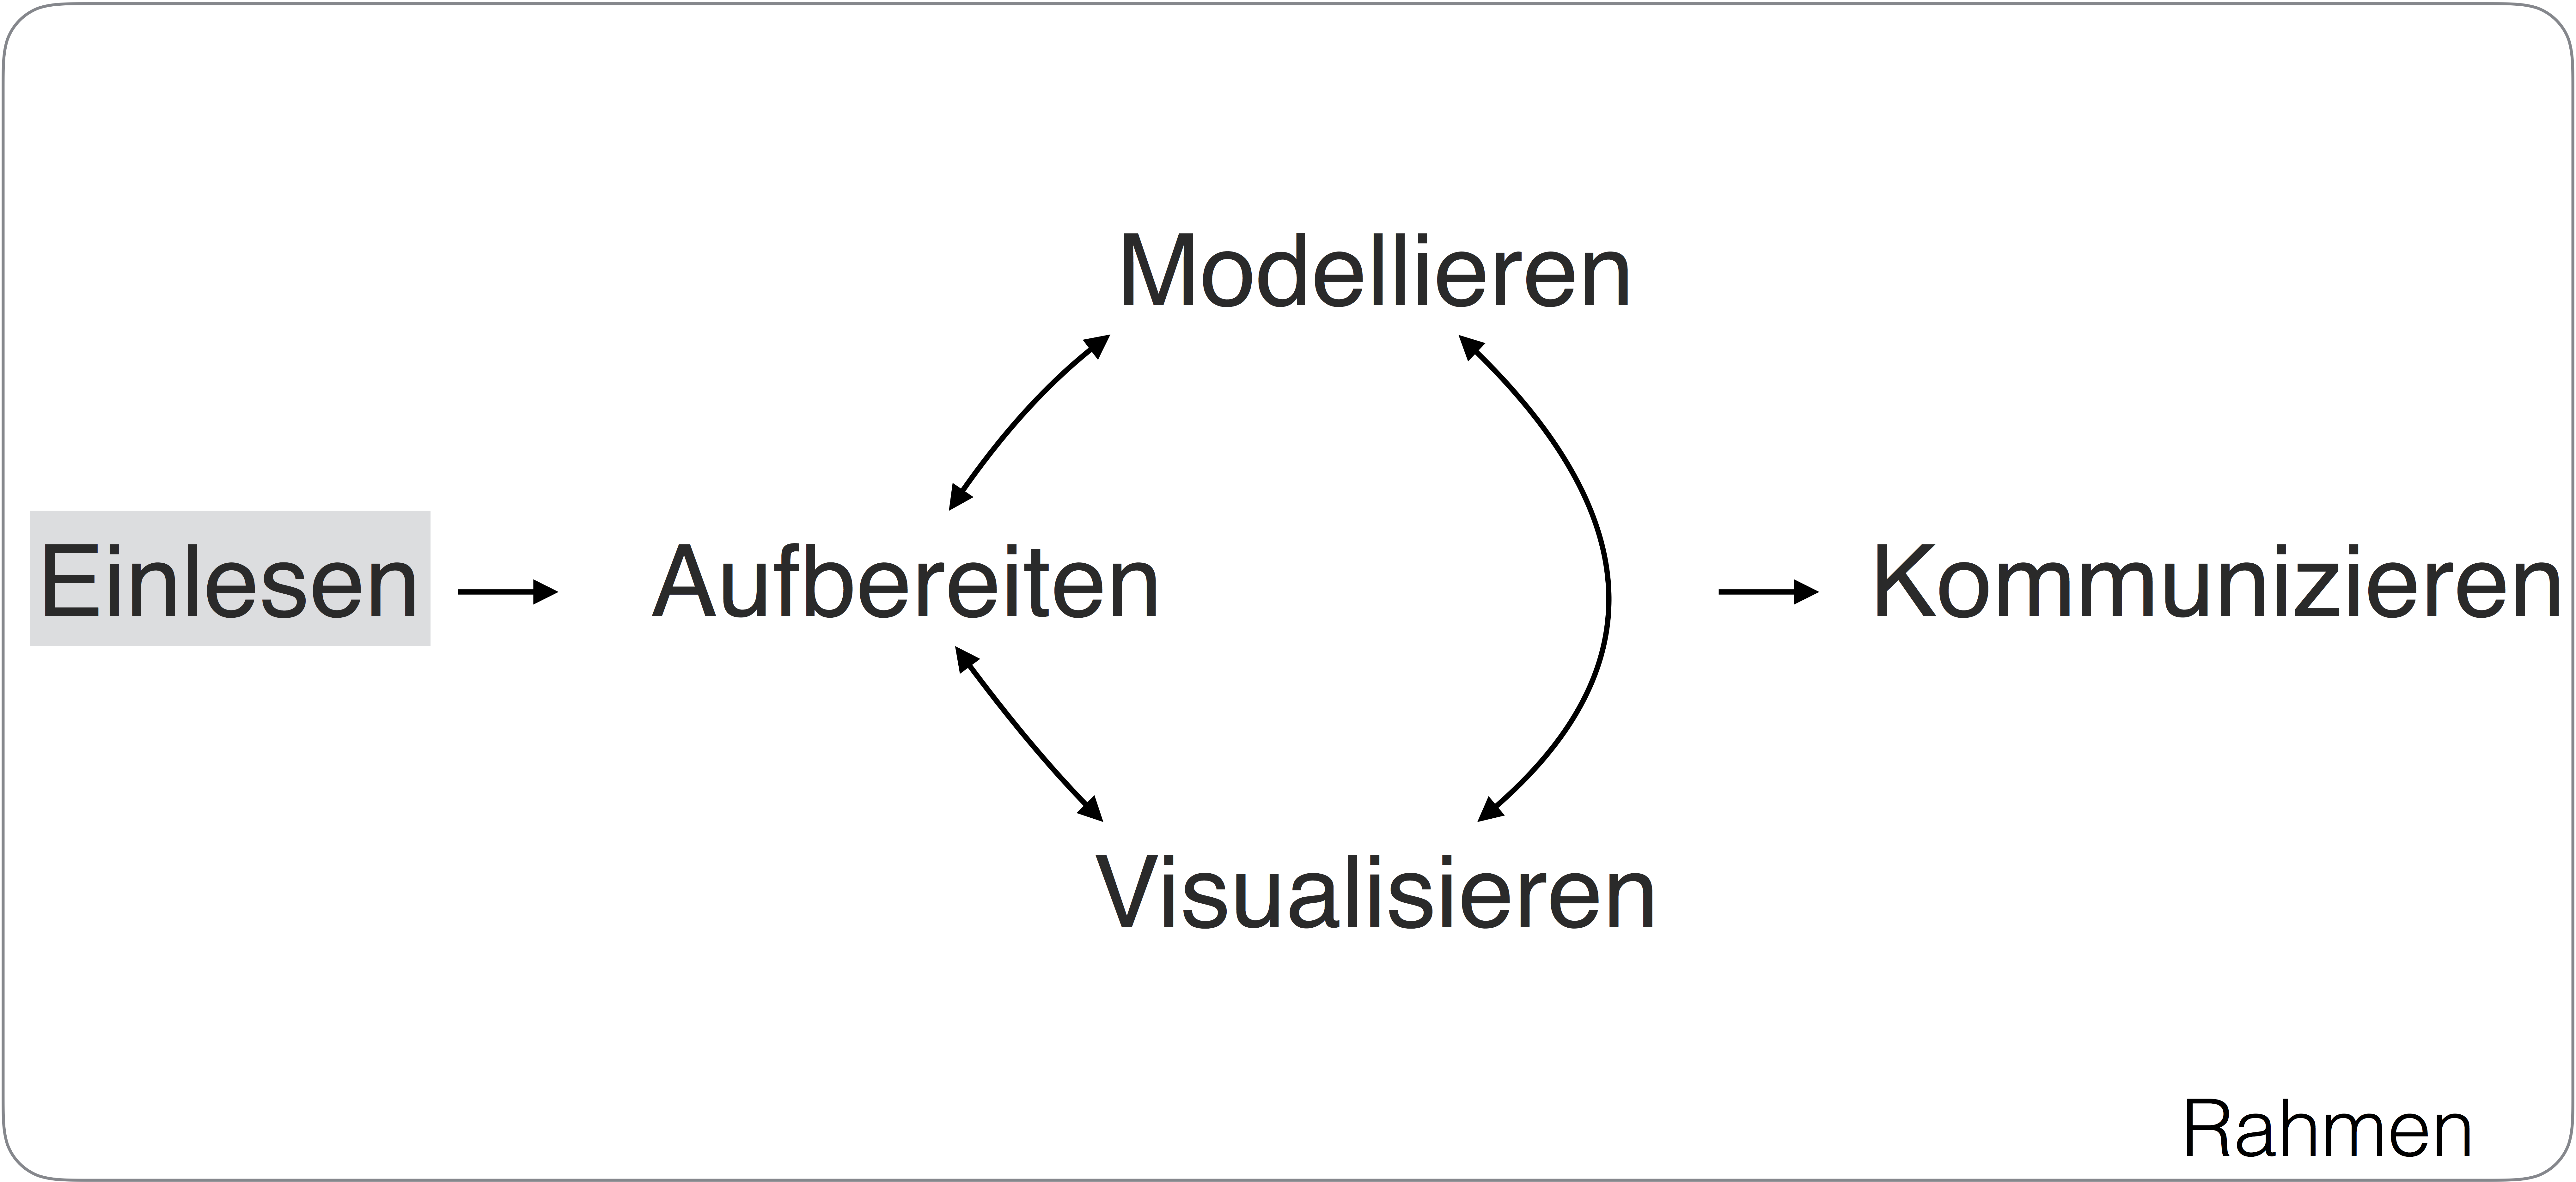
\includegraphics[width=0.8\linewidth]{../images/tidy/Einlesen} 

}

\caption{Daten sauber einlesen}\label{fig:step-Einlesen}
\end{figure}

\end{frame}

\begin{frame}{Daten (CSV, XLS,\ldots{}) mit RStudio importieren}

\begin{figure}

{\centering 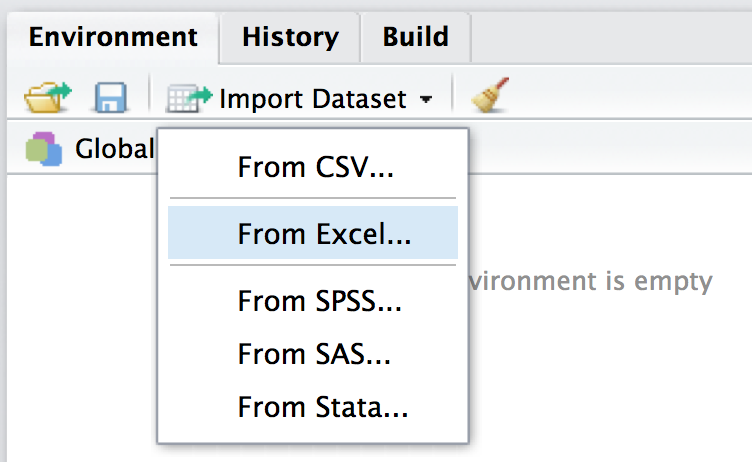
\includegraphics[width=0.5\linewidth]{../images/tidy/import_RStudio} 

}

\caption{Daten einlesen (importieren) mit RStudio}\label{fig:data-import-RStudio}
\end{figure}

\end{frame}

\begin{frame}[fragile]{CSV-Dateien sind einer der wichtigsten
Daten-Formate}

\begin{verbatim}
row_number,date_time,study_time,self_eval,interest,score
1,05.01.2017 13:57:01,5,8,5,29
2,05.01.2017 21:07:56,3,7,3,29
3,05.01.2017 23:33:47,5,10,6,40
4,06.01.2017 09:58:05,2,3,2,18
5,06.01.2017 14:13:08,4,8,6,34
6,06.01.2017 14:21:18,NA,NA,NA,39
\end{verbatim}

\end{frame}

\begin{frame}{Das Arbeitsverzeichnis mit RStudio wählen}

\begin{figure}

{\centering 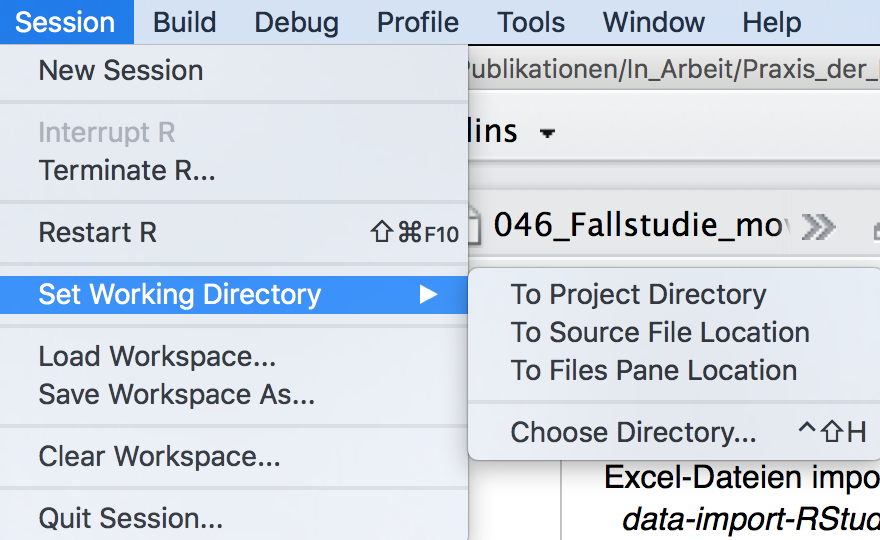
\includegraphics[width=0.5\linewidth]{../images/tidy/Arbeitsverzeichnis} 

}

\caption{Das Arbeitsverzeichnis mit RStudio auswählen}\label{fig:Arbeitsverzeichnis}
\end{figure}

\end{frame}

\begin{frame}{Normalform einer Tabelle}

\begin{figure}

{\centering 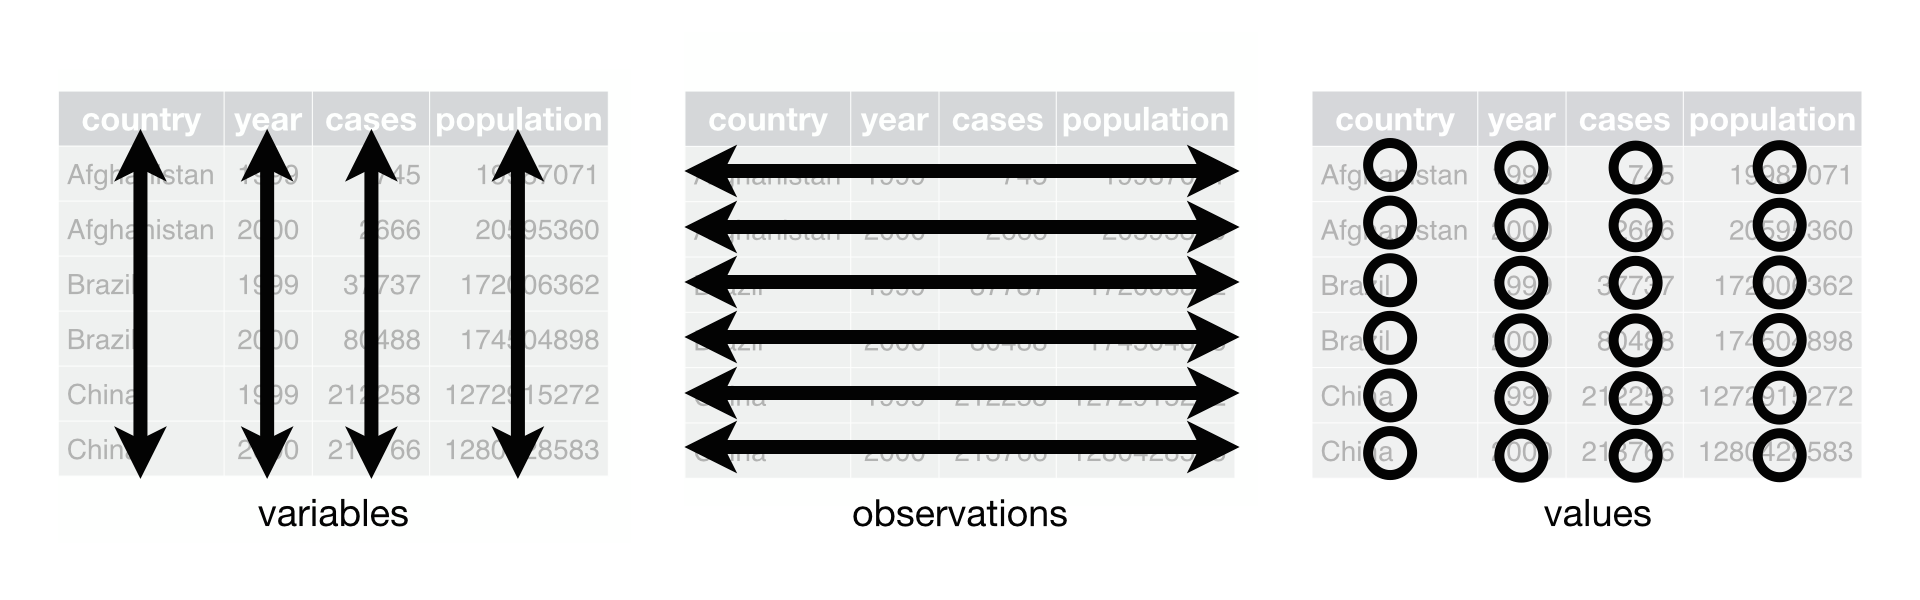
\includegraphics[width=0.8\linewidth]{../images/tidy/tidy-1} 

}

\caption{Schematische Darstellung eines Dataframes in Normalform}\label{fig:tidy1}
\end{figure}

\end{frame}

\begin{frame}{Breit vs.~Lang}

\begin{figure}

{\centering 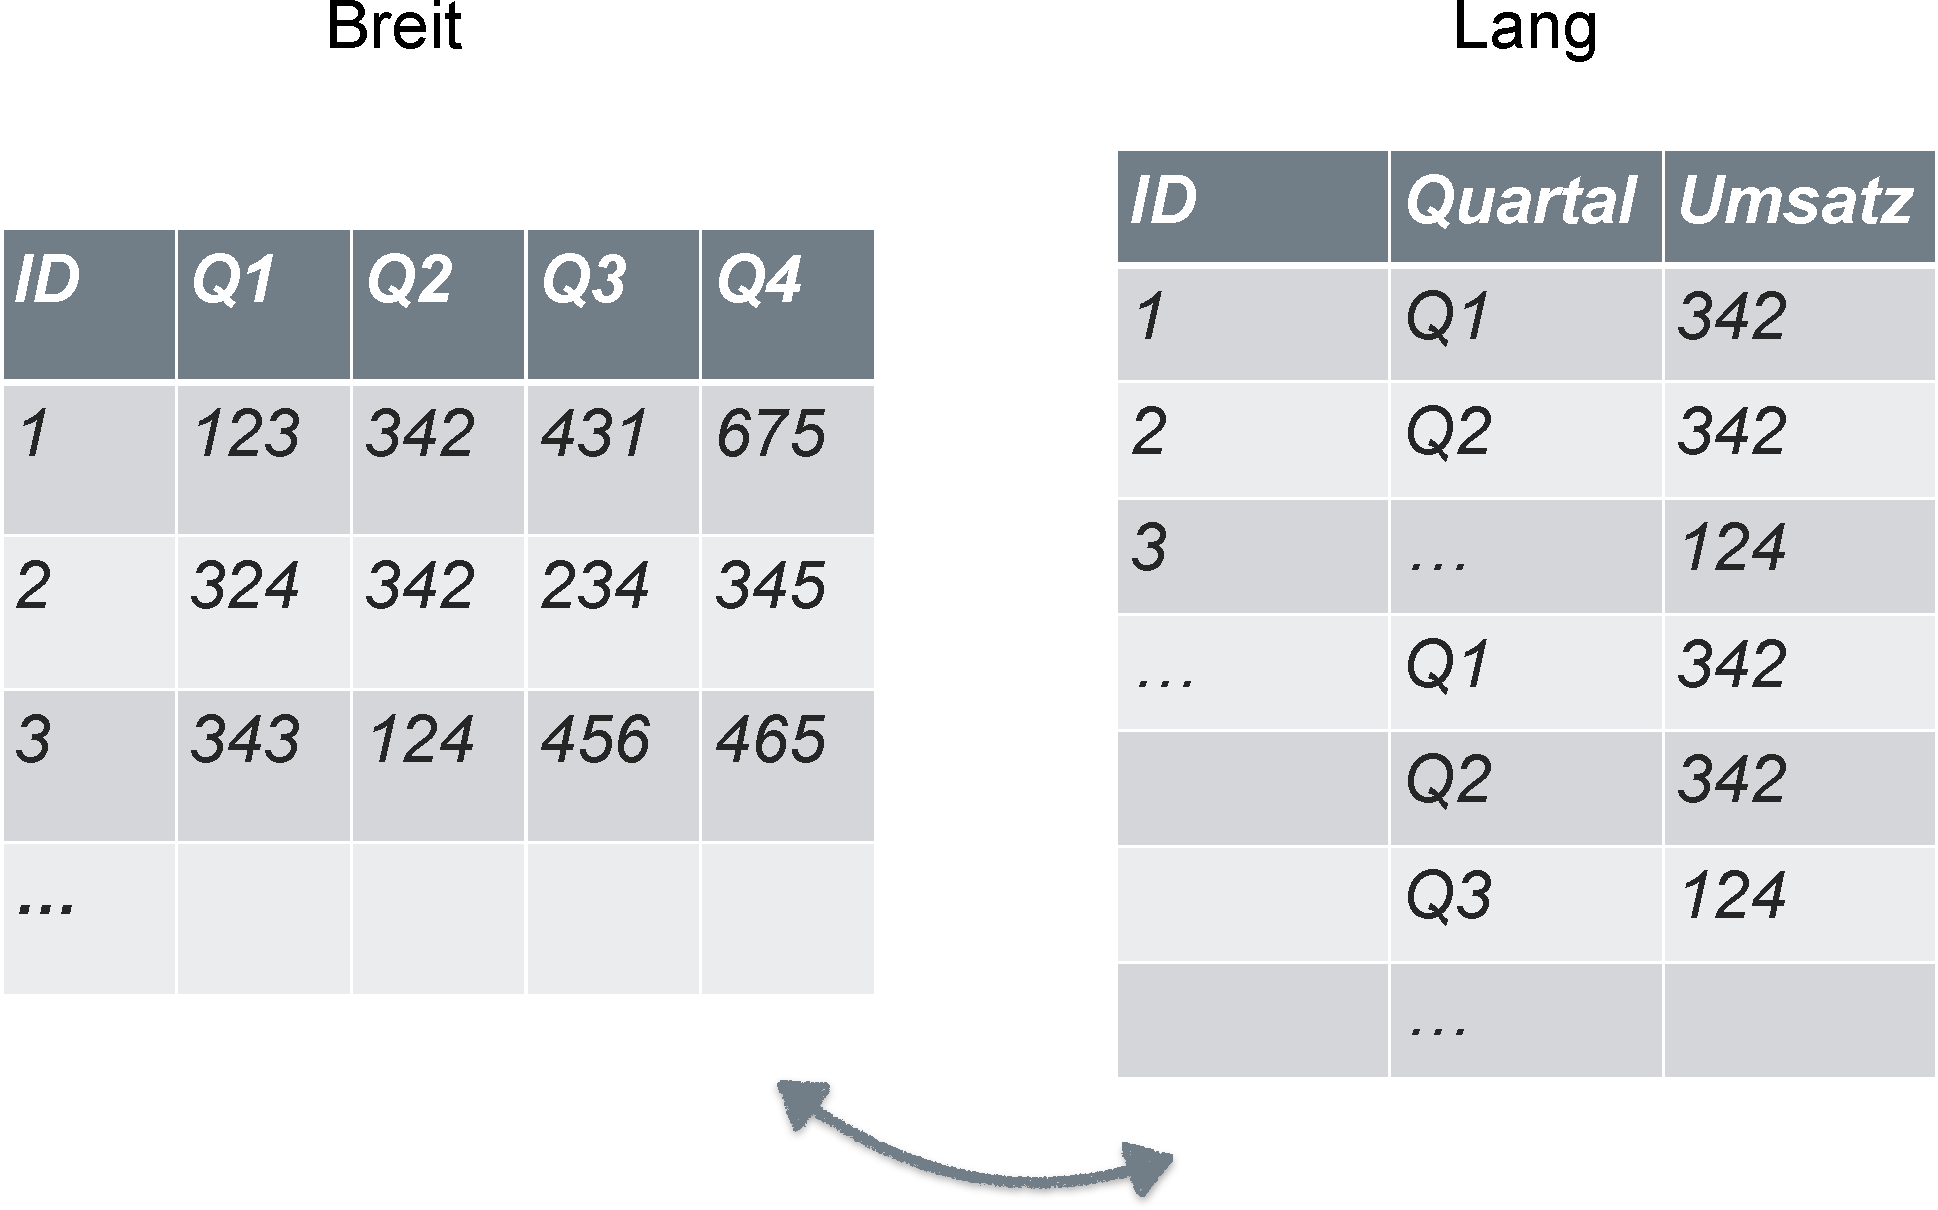
\includegraphics[width=0.8\linewidth]{../images/tidy/breit_lang} 

}

\caption{Dieselben Daten - einmal breit, einmal lang}\label{fig:lang-breit}
\end{figure}

\end{frame}

\begin{frame}{Ein Dataframe in Normalform - Beispiel}

\begin{figure}

{\centering 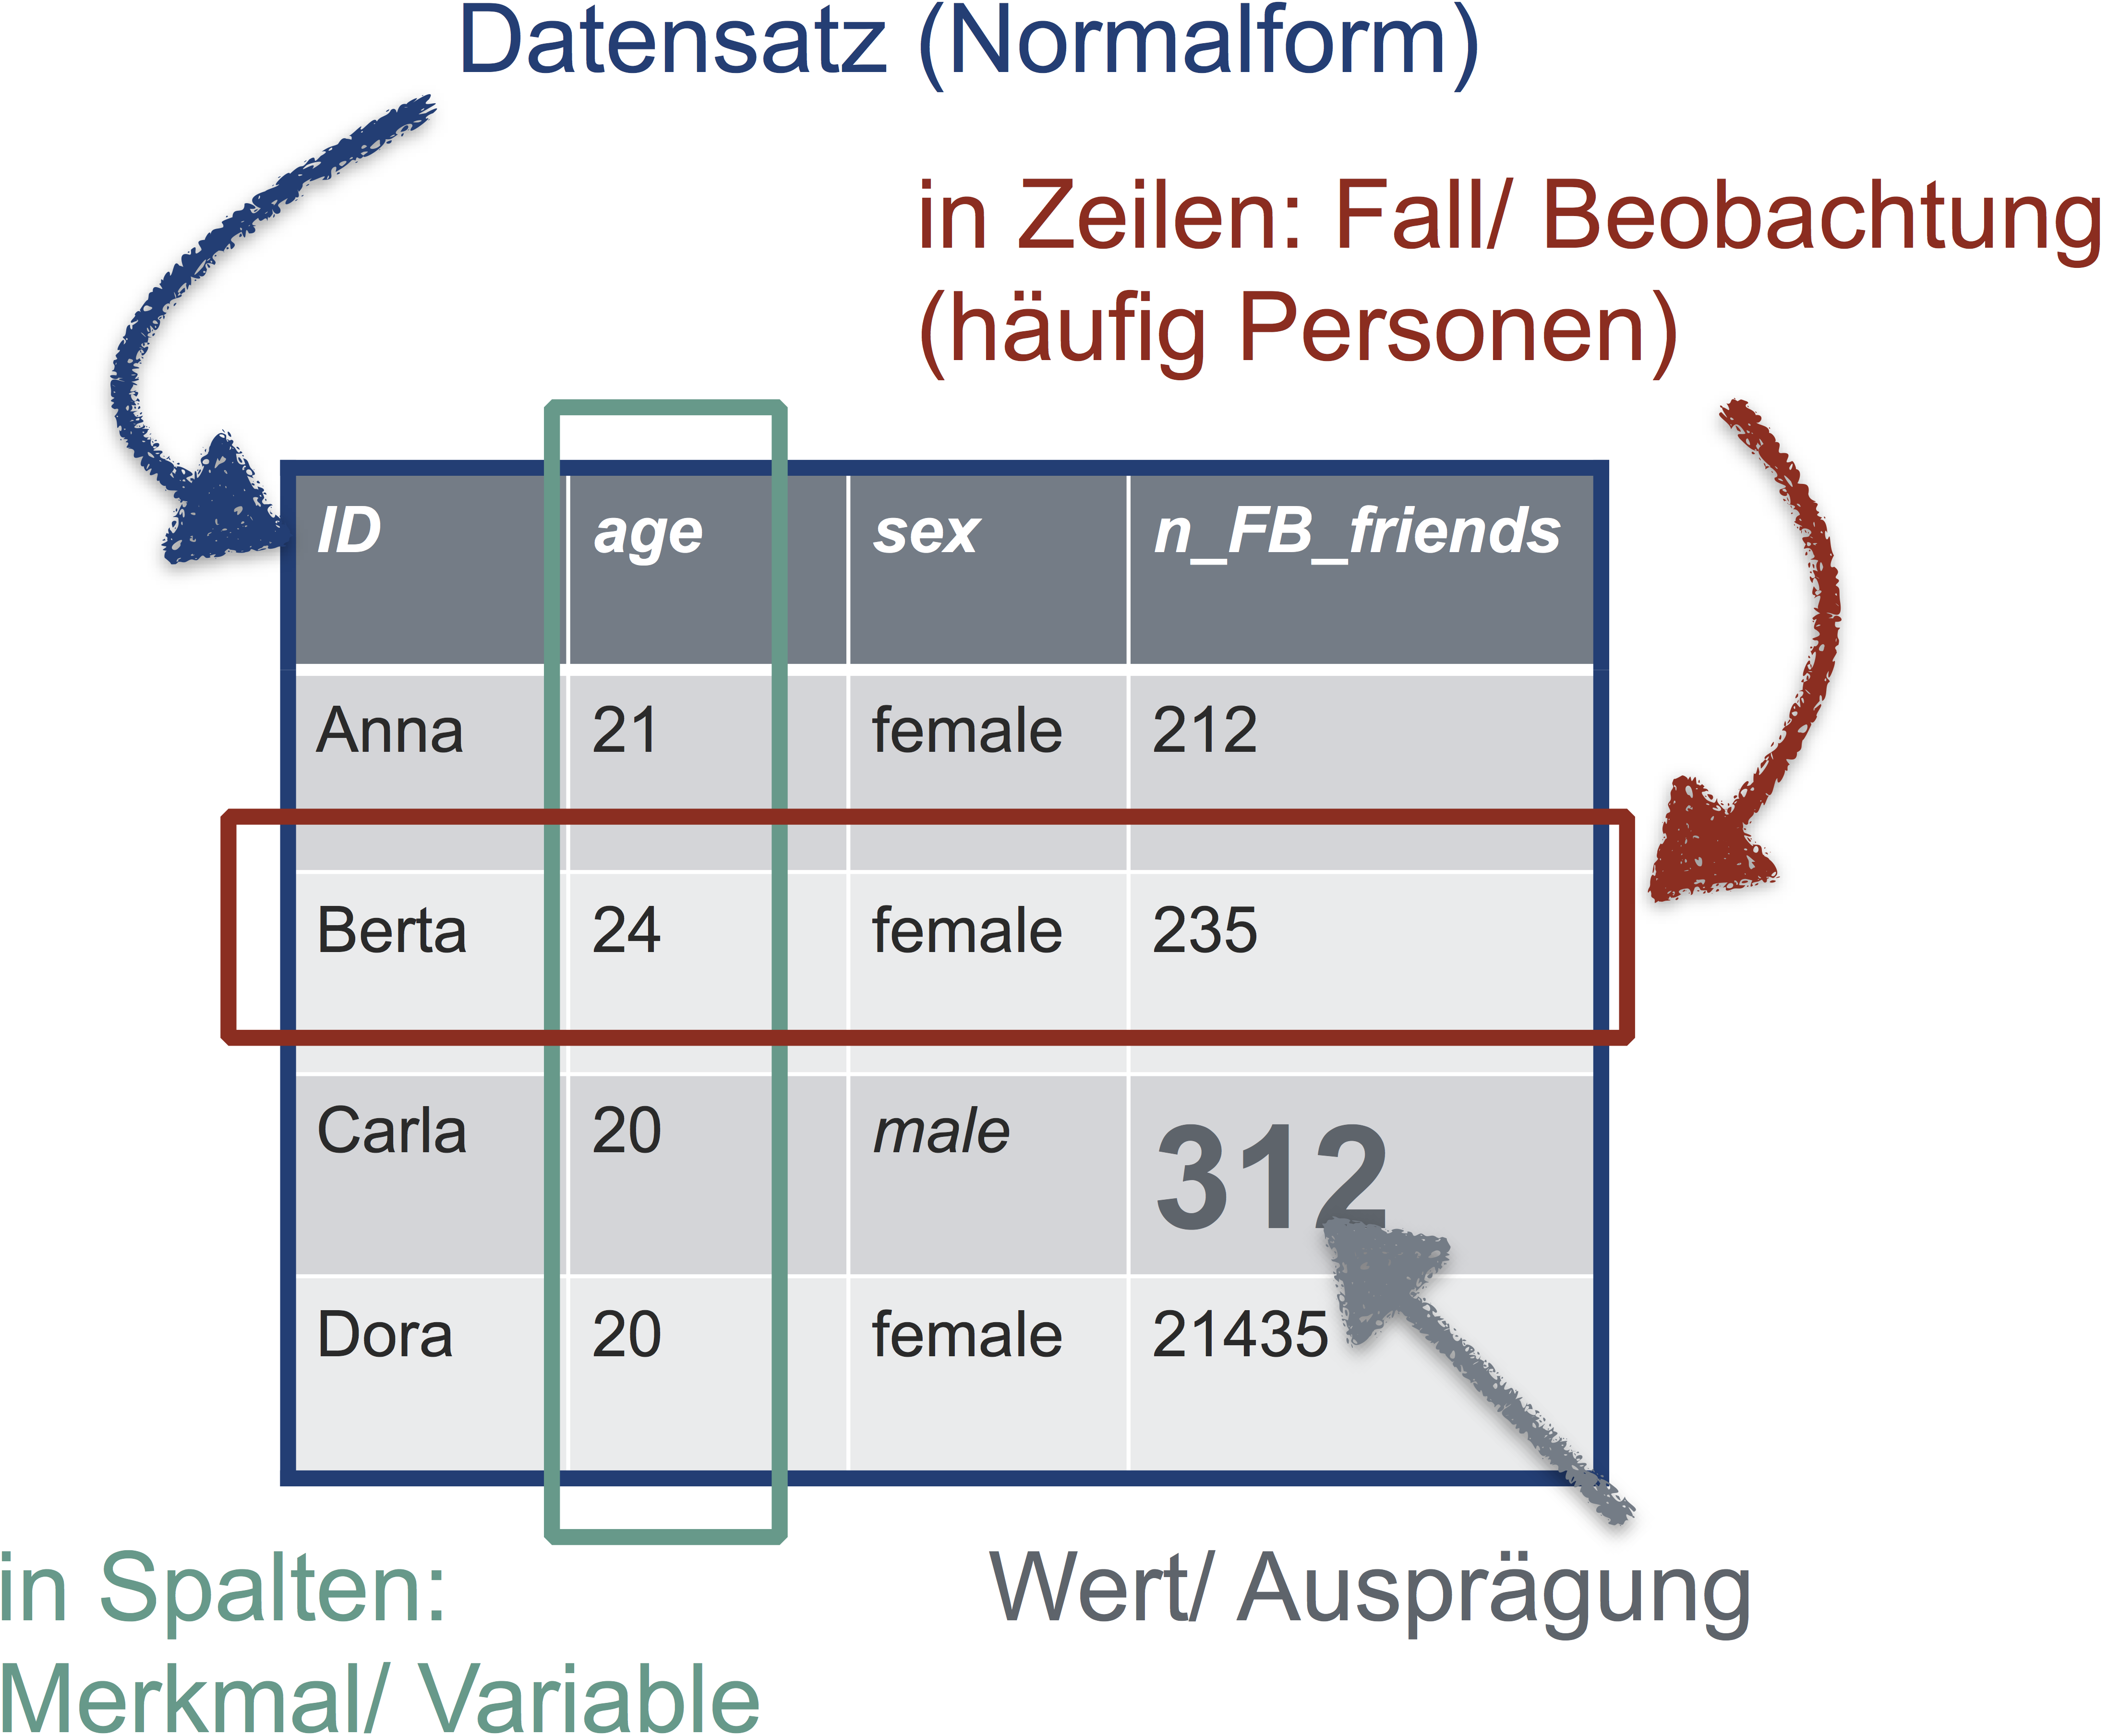
\includegraphics[width=0.4\linewidth]{../images/tidy/Normalform} 

}

\caption{Illustration eines Datensatzes in Normalform}\label{fig:fig-Normalform}
\end{figure}

\end{frame}

\begin{frame}{Tabelle in Normalform bringen}

\begin{figure}

{\centering 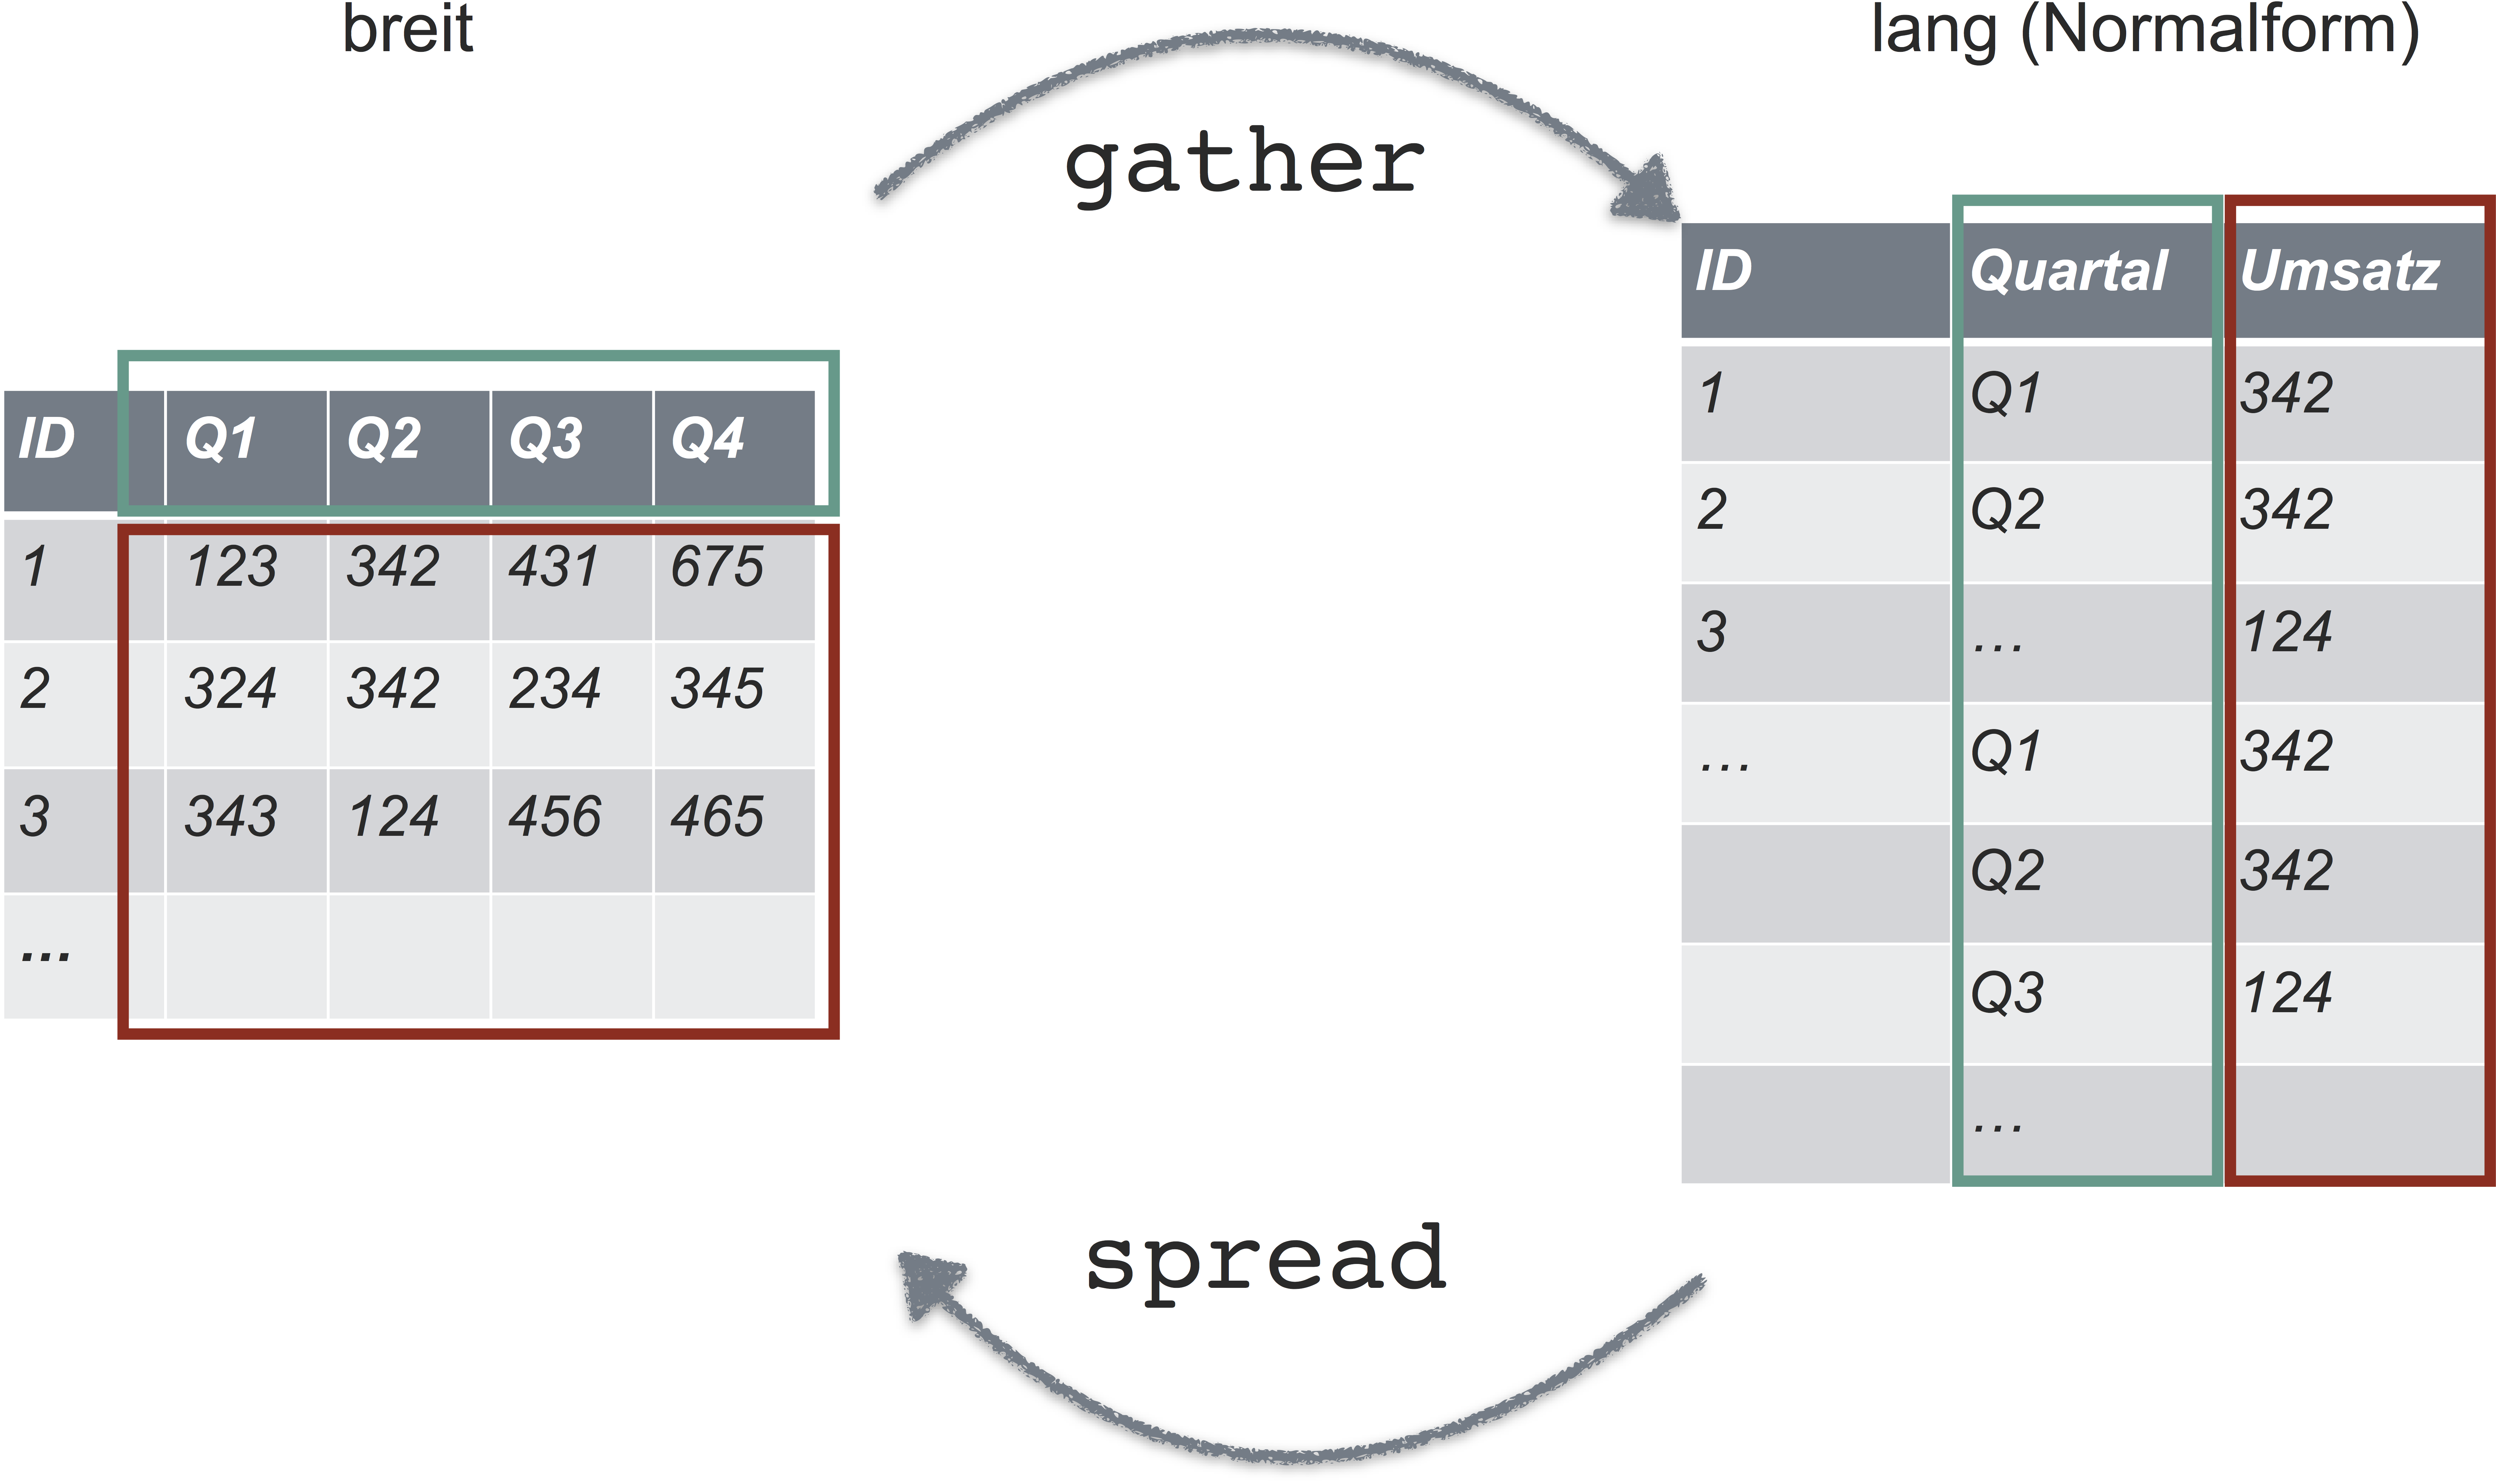
\includegraphics[width=0.8\linewidth]{../images/tidy/gather_spread-crop} 

}

\caption{Mit 'gather' und 'spread' wechselt man von der breiten Form zur langen Form}\label{fig:gather-spread}
\end{figure}

\end{frame}

\begin{frame}{Beispiel für die Normalisierung einer Tabelle}

\begin{figure}

{\centering 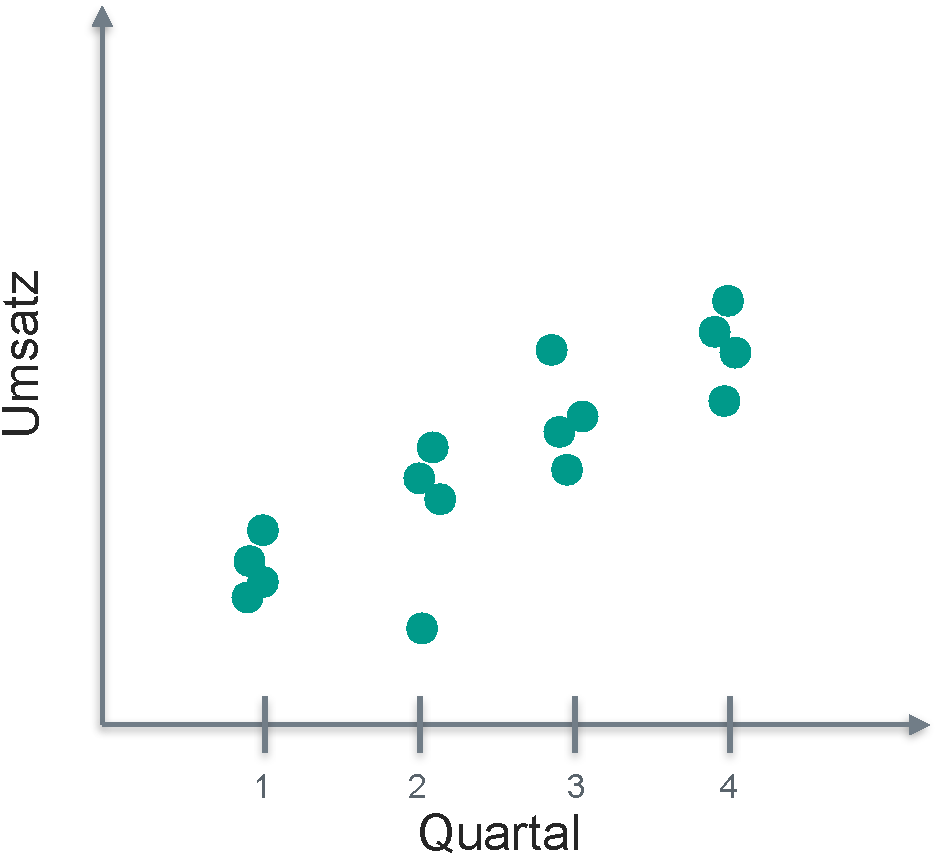
\includegraphics[width=0.5\linewidth]{../images/tidy/bsp_diagramm-crop} 

}

\caption{Ein Beispiel für eine Abbildung zu einer Normalform-Tabelle}\label{fig:bsp-abb}
\end{figure}

\end{frame}

\begin{frame}[fragile]{\texttt{gather} und \texttt{spread}}

\begin{Shaded}
\begin{Highlighting}[]
\NormalTok{df_lang <-}\StringTok{ }\KeywordTok{gather}\NormalTok{(df_breit, }\DataTypeTok{key =} \StringTok{"Quartal"}\NormalTok{, }\DataTypeTok{value =} \StringTok{"Umsatz"}\NormalTok{)}

\NormalTok{df_breit <-}\StringTok{ }\KeywordTok{spread}\NormalTok{(df_lang, Quartal, Umsatz)}

<<<<<<< Updated upstream
\NormalTok{df_lang <-}\StringTok{ }\KeywordTok{gather}\NormalTok{(df_breit, }\DataTypeTok{key =} \StringTok{"Quartal"}\NormalTok{, }\DataTypeTok{value =} \StringTok{"Umsatz"}\NormalTok{, }\OperatorTok{-}\NormalTok{ID)}
=======
\NormalTok{df_lang <-}\StringTok{ }\KeywordTok{gather}\NormalTok{(df_breit, }\DataTypeTok{key =} \StringTok{"Quartal"}\NormalTok{, }\DataTypeTok{value =} \StringTok{"Umsatz"}\NormalTok{, -ID)}
>>>>>>> Stashed changes
\end{Highlighting}
\end{Shaded}

\end{frame}

\begin{frame}[fragile]{Textkodierung und Daten exportieren}

\begin{quote}
Speichern Sie R-Textdateien wie Skripte stets mit UTF-8-Kodierung ab.
\end{quote}

\begin{Shaded}
\begin{Highlighting}[]
\KeywordTok{write.csv}\NormalTok{(name_der_tabelle, }\StringTok{"Dateiname.csv"}\NormalTok{)}
\end{Highlighting}
\end{Shaded}

\end{frame}

\section{Datenjudo}\label{datenjudo}

\begin{frame}[fragile]{Lernziele für das Kapitel `Datenjudo'}

\begin{itemize}
\tightlist
\item
  Die zentralen Ideen der Datenanalye mit dplyr verstehen.
\item
  Typische Probleme der Datenanalyse schildern können.
\item
  Zentrale \texttt{dplyr}-Befehle anwenden können.
\item
  \texttt{dplyr}-Befehle kombinieren können.
\item
  Die Pfeife anwenden können.
\item
  Werte umkodieren und ``binnen'' können.
\end{itemize}

\end{frame}

\begin{frame}{Prozess der Datenanalyse -- Datenjudo}

\begin{figure}

{\centering 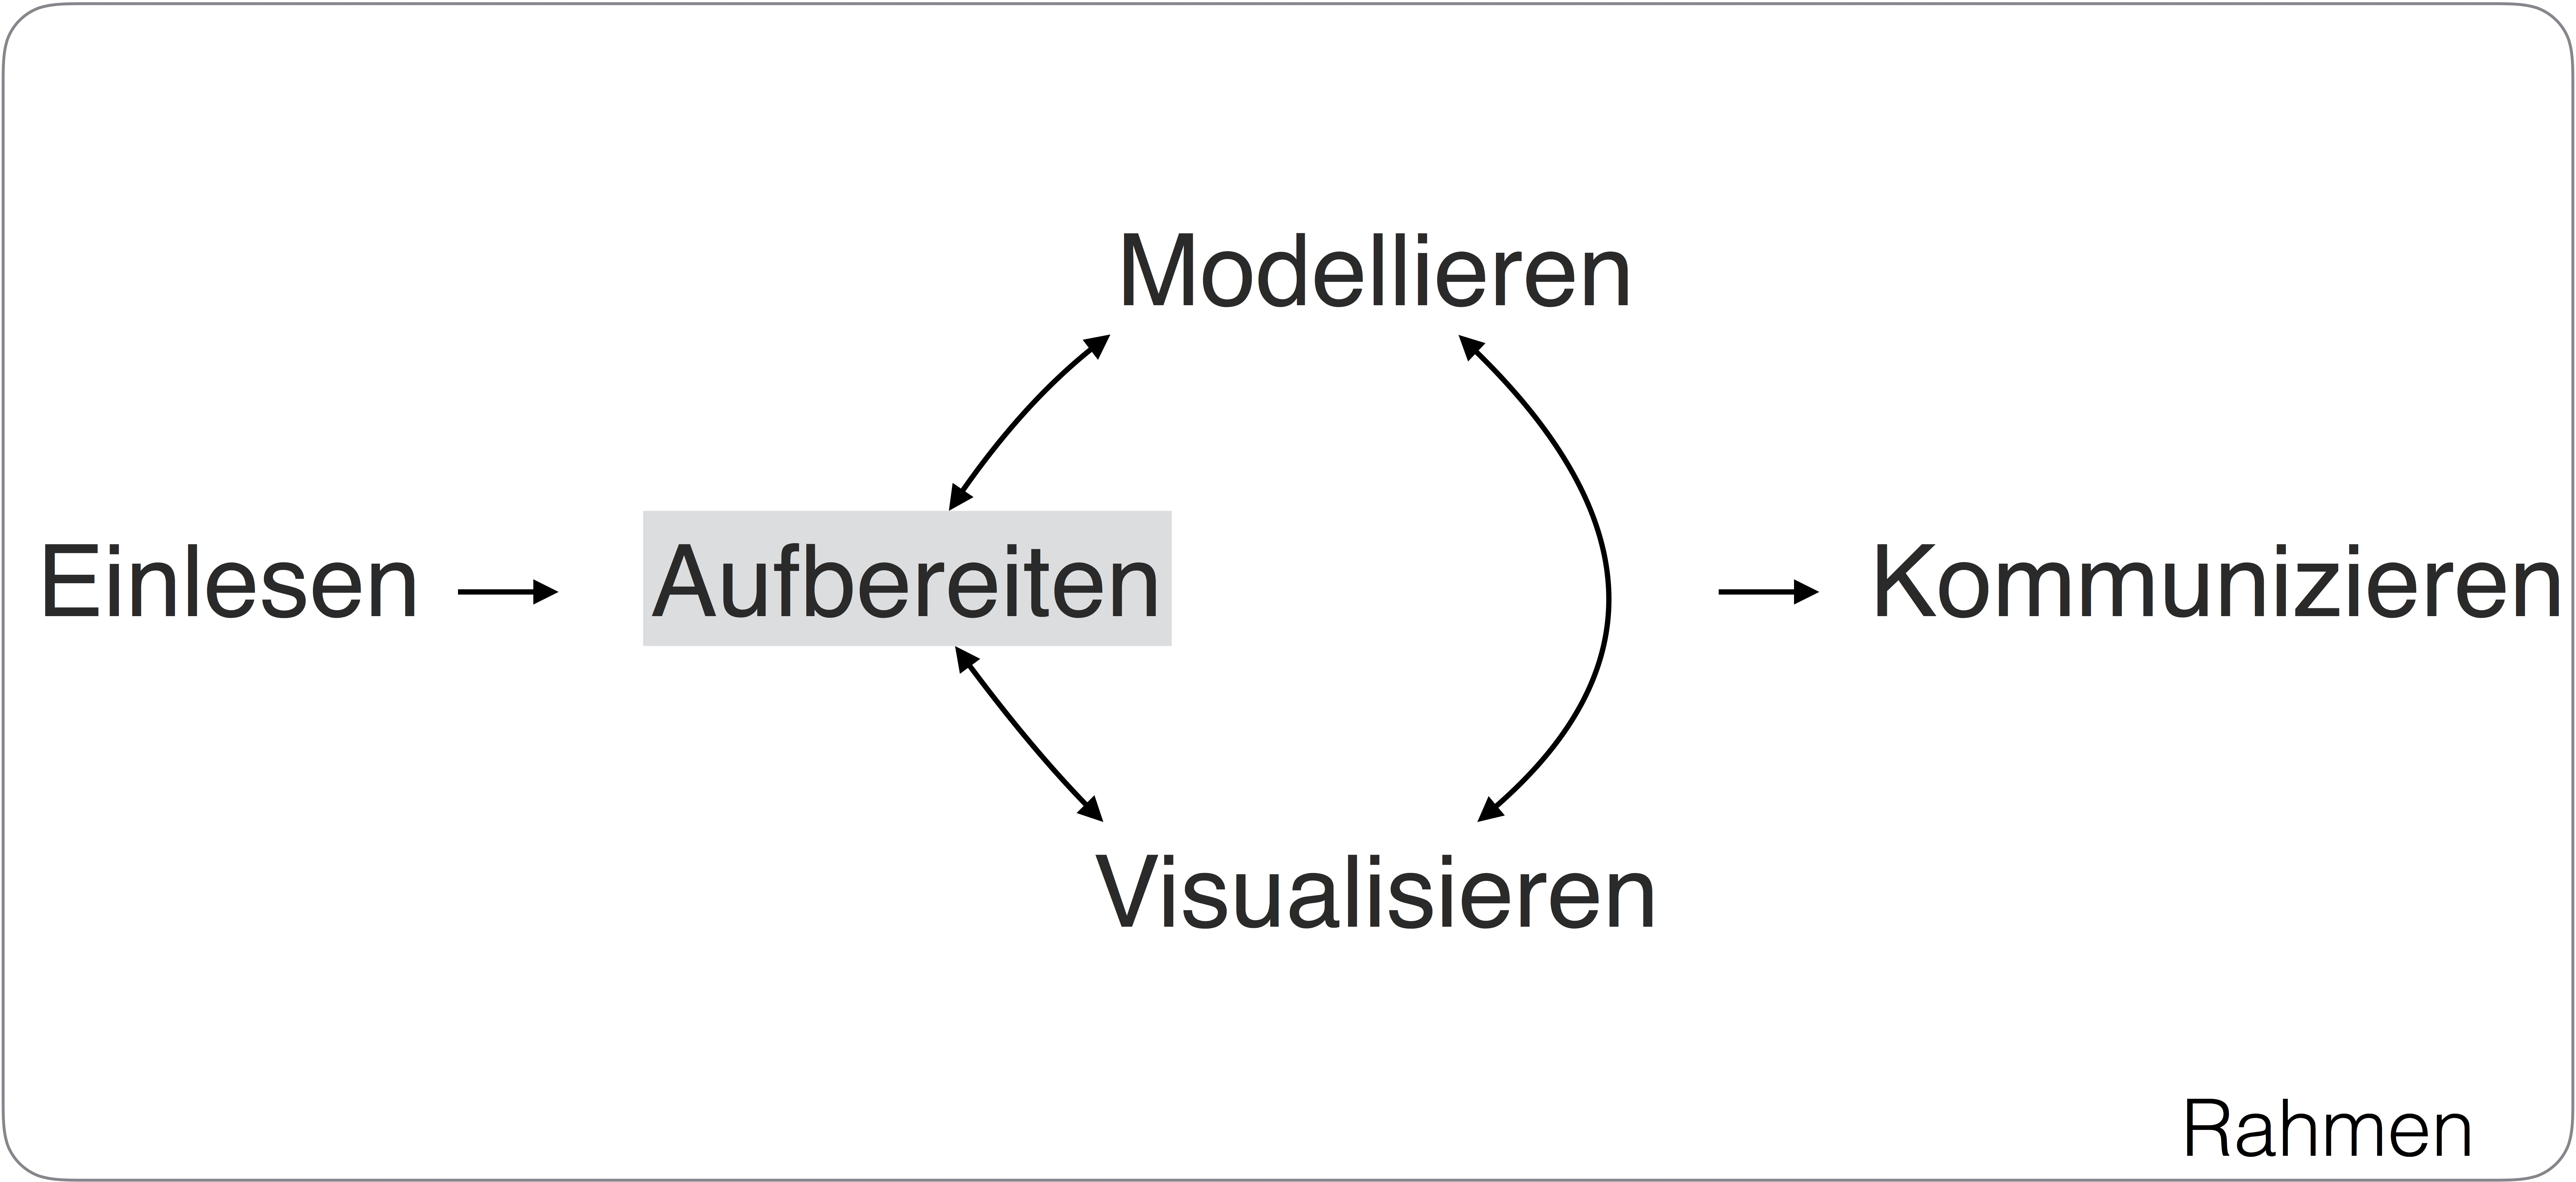
\includegraphics[width=0.8\linewidth]{../images/Datenjudo/Aufbereiten} 

}

\caption{Daten aufbereiten}\label{fig:fig-datenjudo}
\end{figure}

\end{frame}

\begin{frame}{Typische Probleme bei der Datenaufbereitung}

Typische Probleme, die immer wieder auftreten, sind:

\begin{itemize}
\tightlist
\item
  \emph{Fehlende Werte}
\item
  \emph{Unerwartete Daten}
\item
  \emph{Daten müssen umgeformt werden}
\item
  \emph{Neue Variablen (Spalten) berechnen}:
\item
  \ldots{}
\end{itemize}

\end{frame}

\begin{frame}{Daten aufbereiten mit \texttt{dplyr}}

\begin{columns}
  \begin{column}{0.49\textwidth}
    
\begin{figure}

{\centering 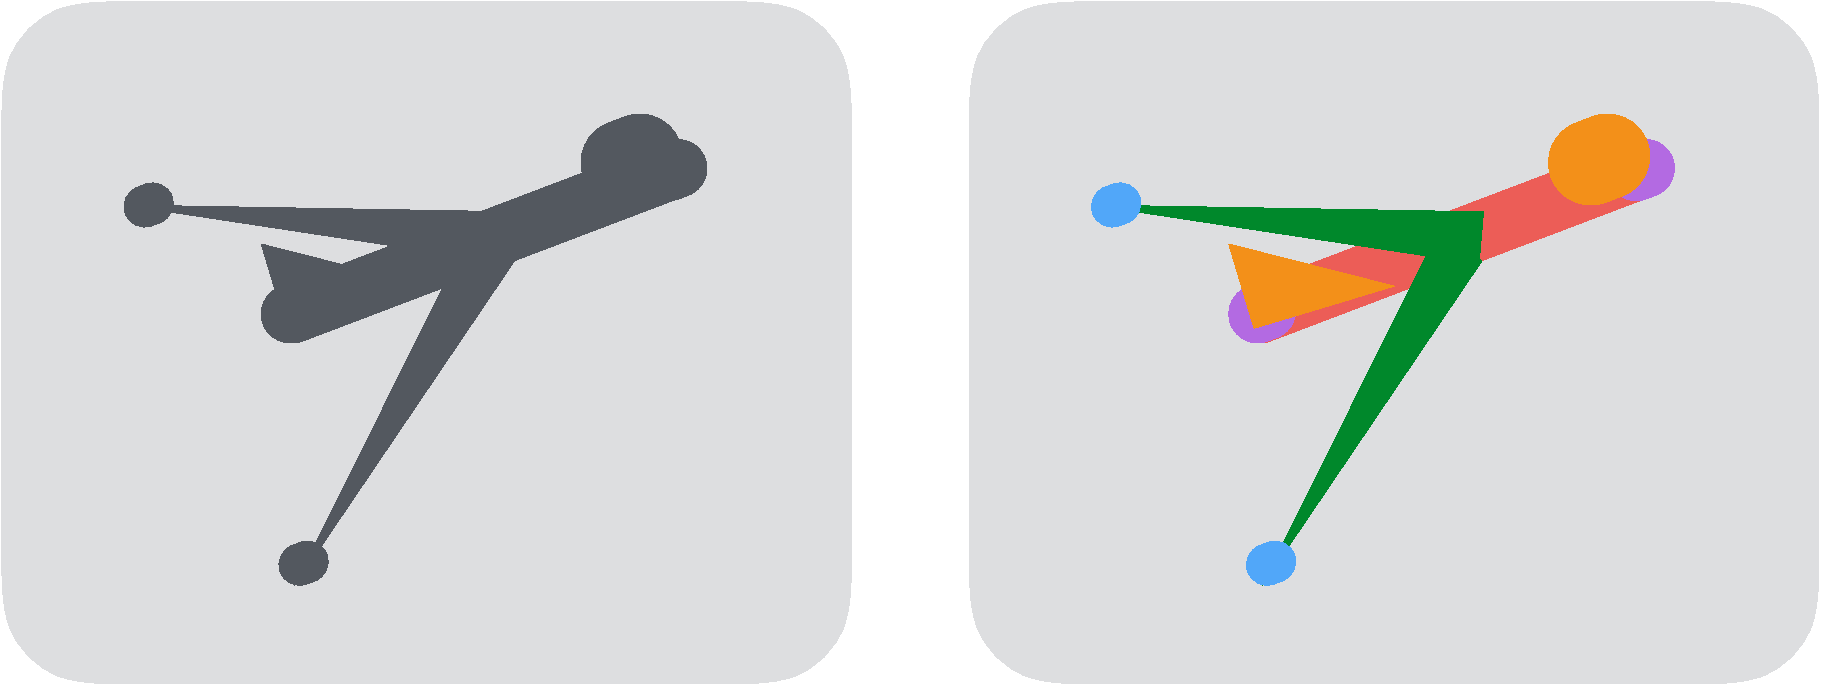
\includegraphics[width=1\linewidth]{../images/Datenjudo/Bausteine_dplyr-crop} 

}

\caption{Lego-Prinzip: Zerlege eine komplexe Struktur in einfache Bausteine}\label{fig:bausteine}
\end{figure}

 \end{column}
  \begin{column}{0.49\textwidth}


\begin{figure}

{\centering 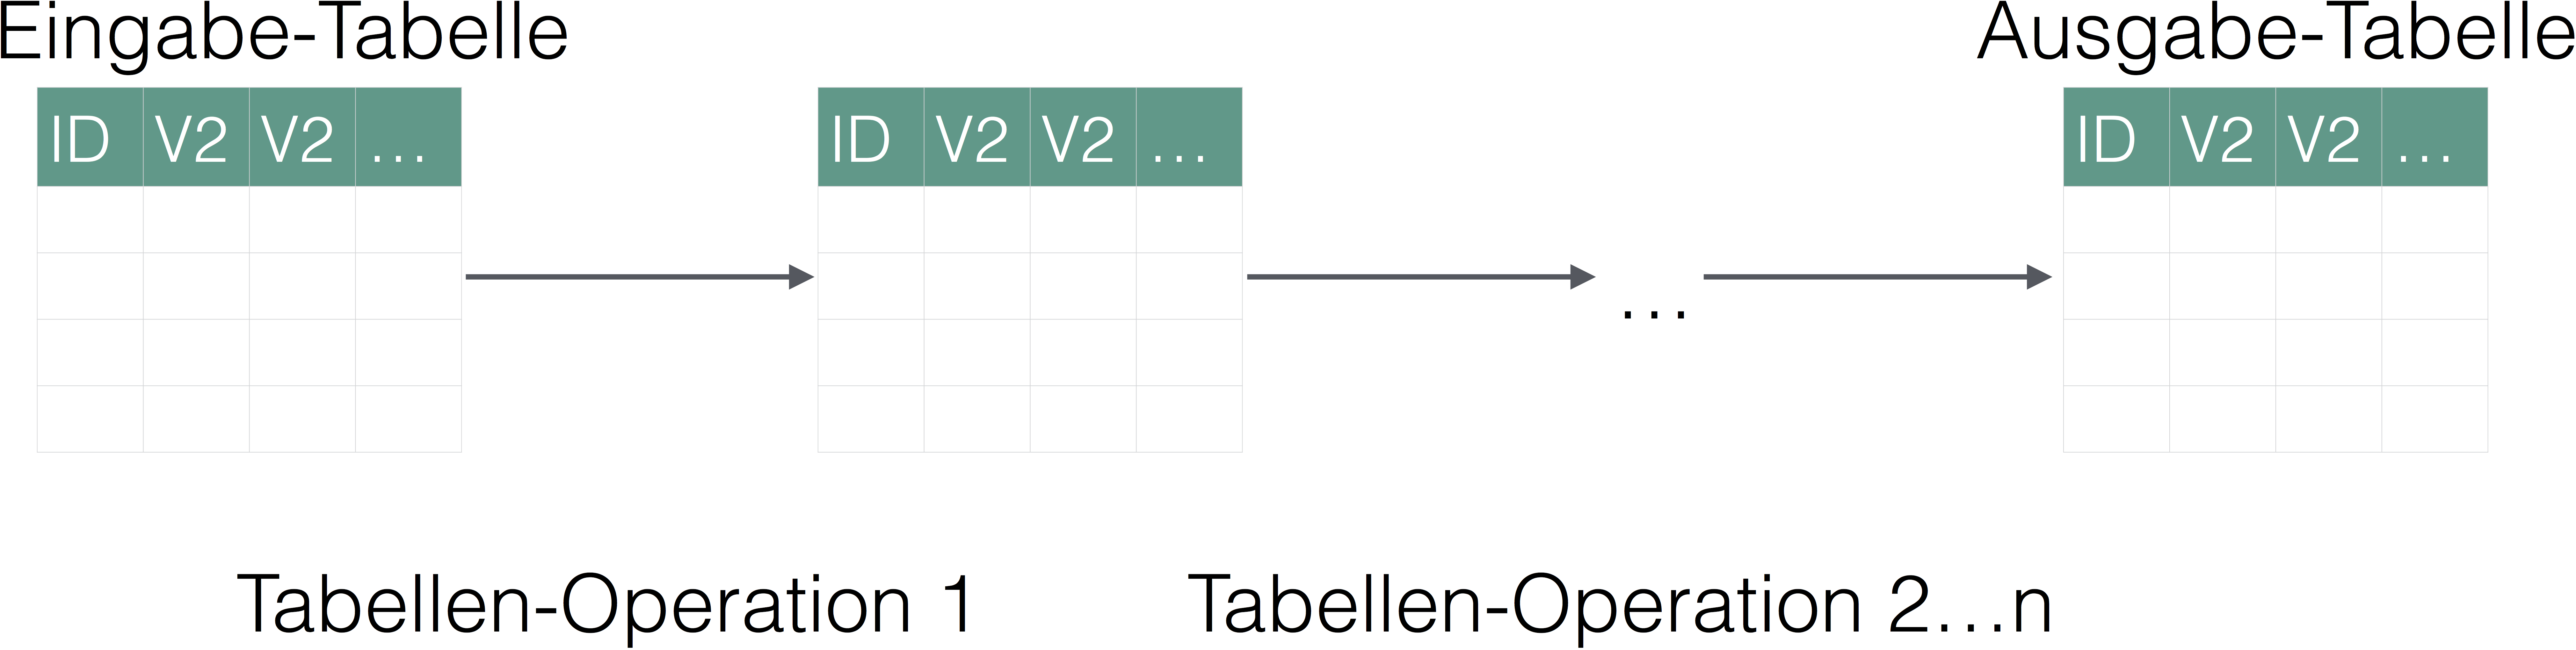
\includegraphics[width=1\linewidth]{../images/Datenjudo/durchpfeifen_allgemein_crop} 

}

\caption{Durchpfeifen: Ein Dataframe wird von Operation zu Operation weitergereicht}\label{fig:durchpfeifen-allgemein}
\end{figure}


  \end{column}
\end{columns}

\end{frame}

\begin{frame}{Zeilen filtern mit \texttt{filter}}

\begin{figure}

{\centering 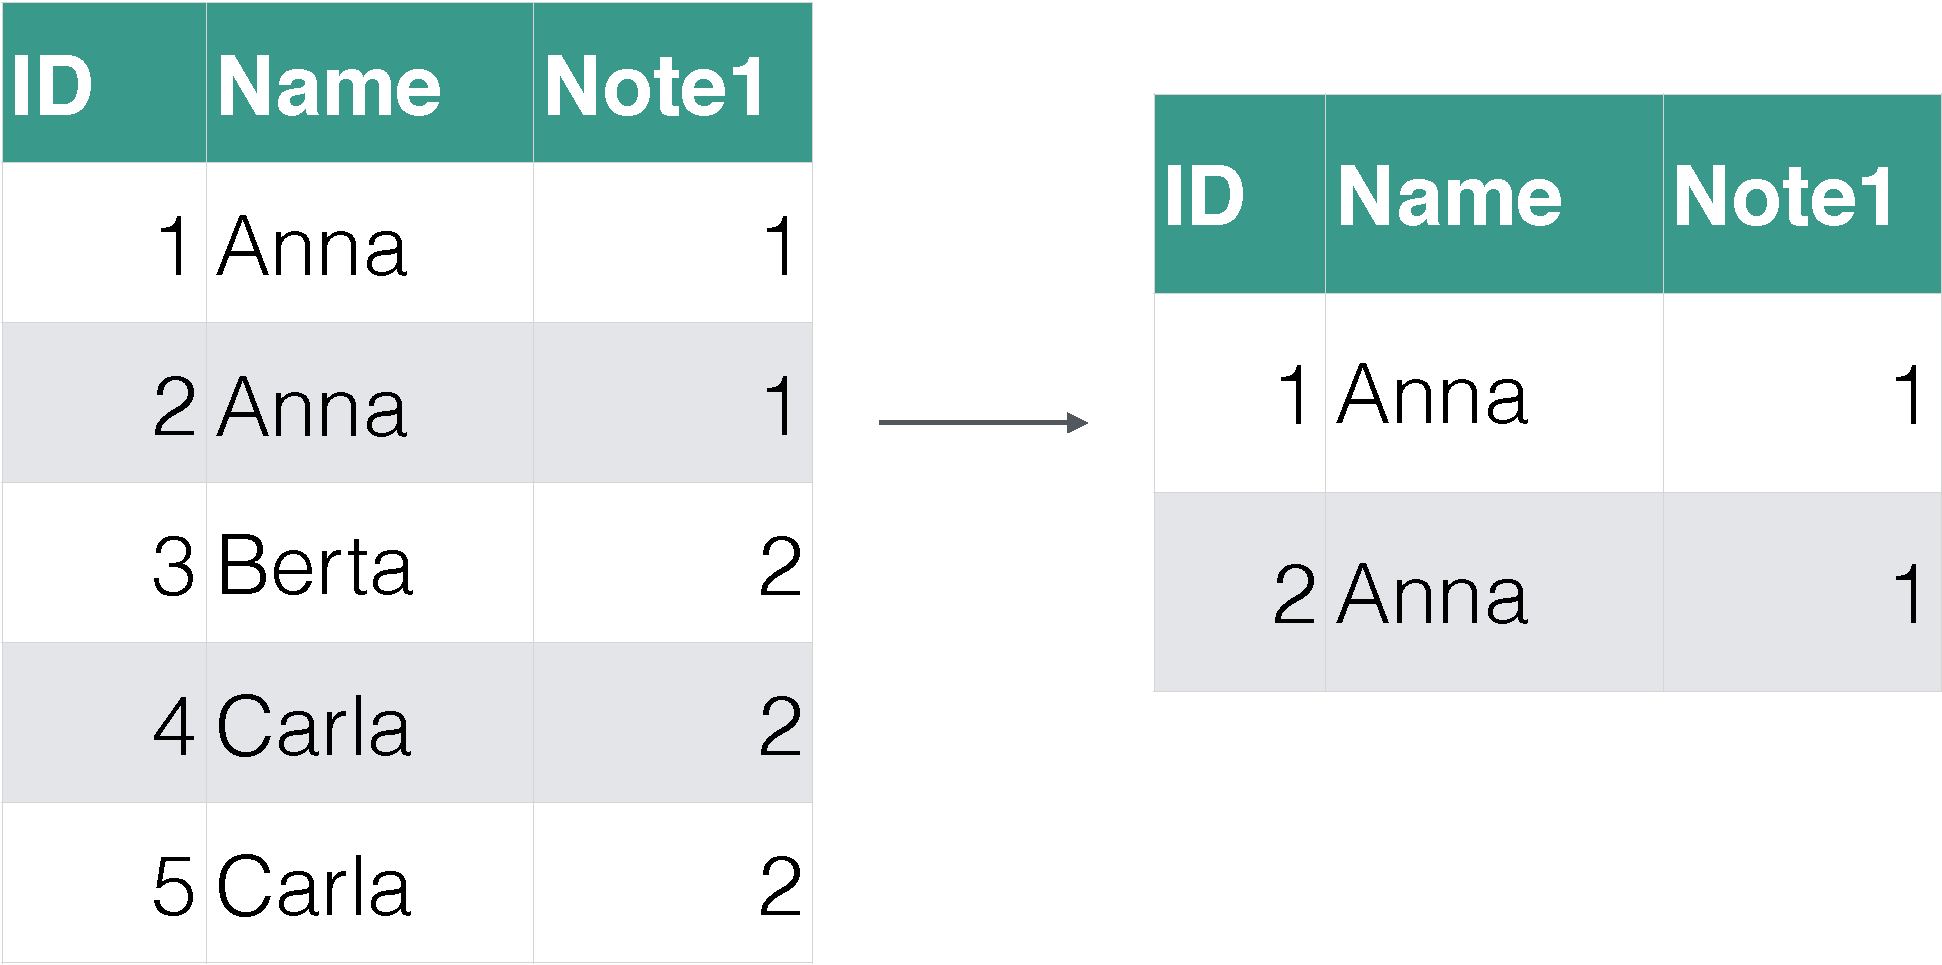
\includegraphics[width=0.8\linewidth]{../images/Datenjudo/filter} 

}

\caption{Zeilen filtern}\label{fig:fig-filter}
\end{figure}

\end{frame}

\begin{frame}{Spalten wählen mit \texttt{select}}

\begin{figure}

{\centering 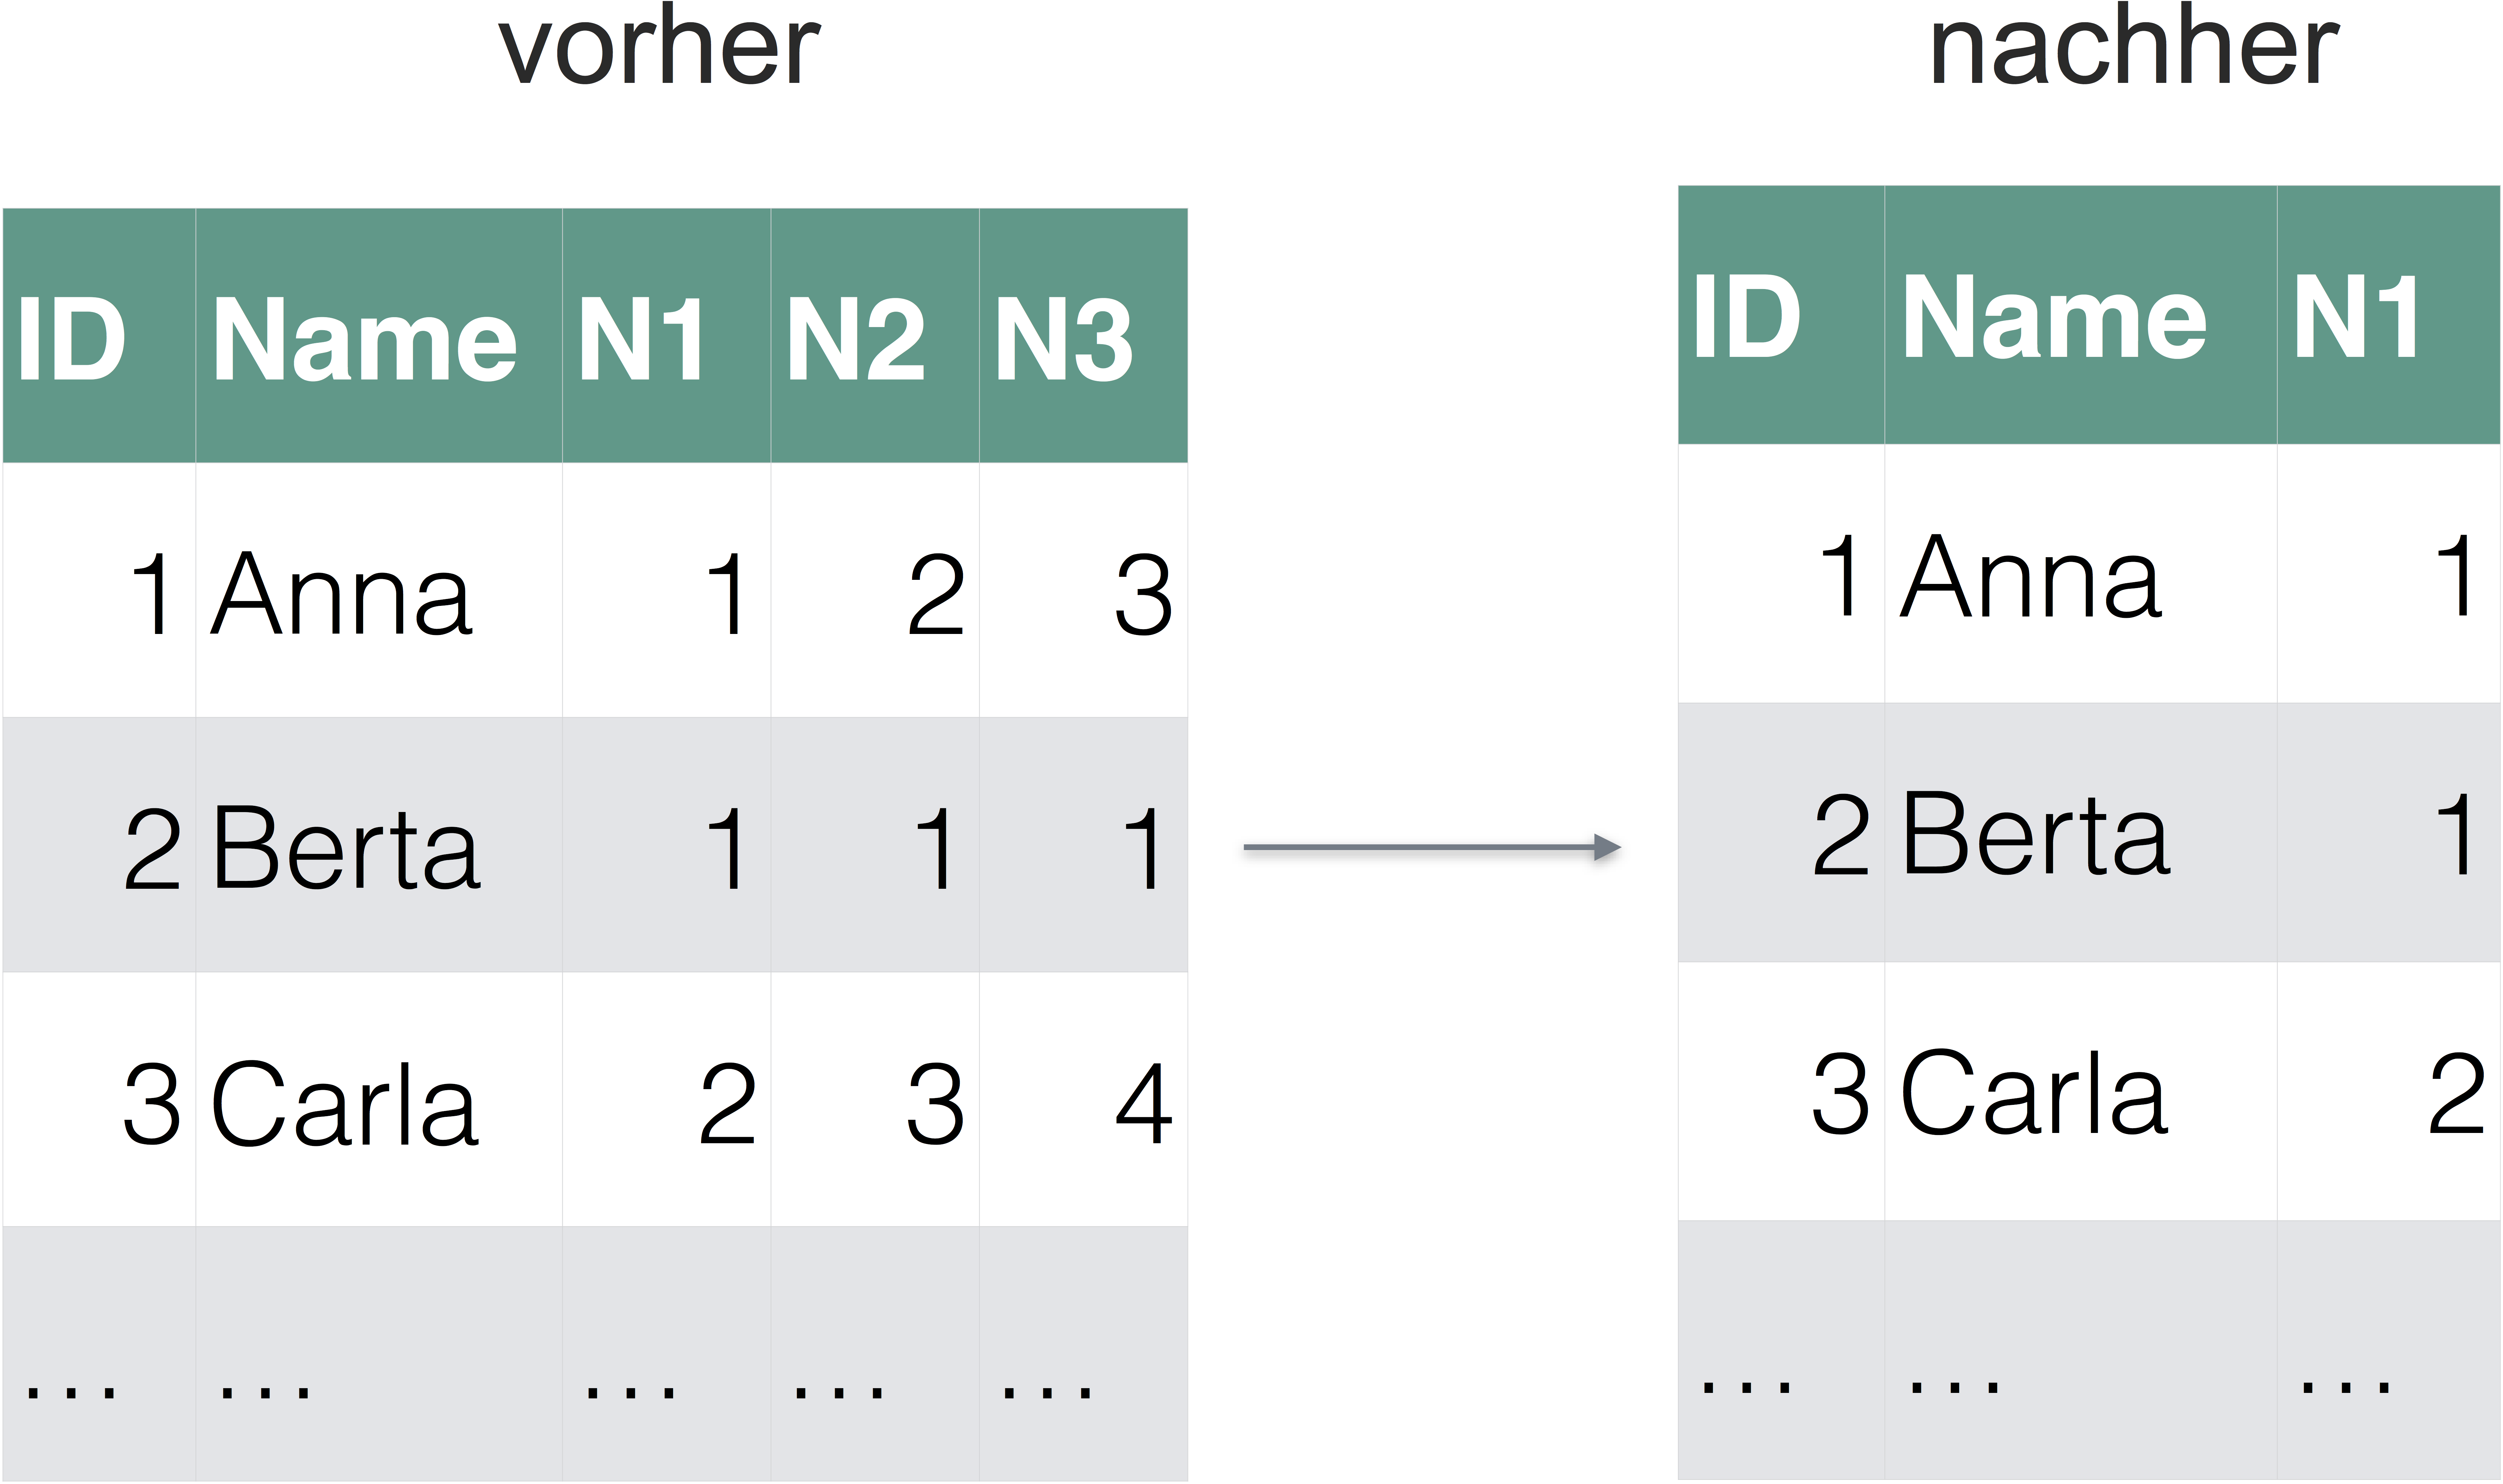
\includegraphics[width=0.8\linewidth]{../images/Datenjudo/select} 

}

\caption{Spalten auswählen}\label{fig:fig-select}
\end{figure}

\end{frame}

\begin{frame}{Zeilen sortieren mit \texttt{arrange}}

\begin{figure}

{\centering 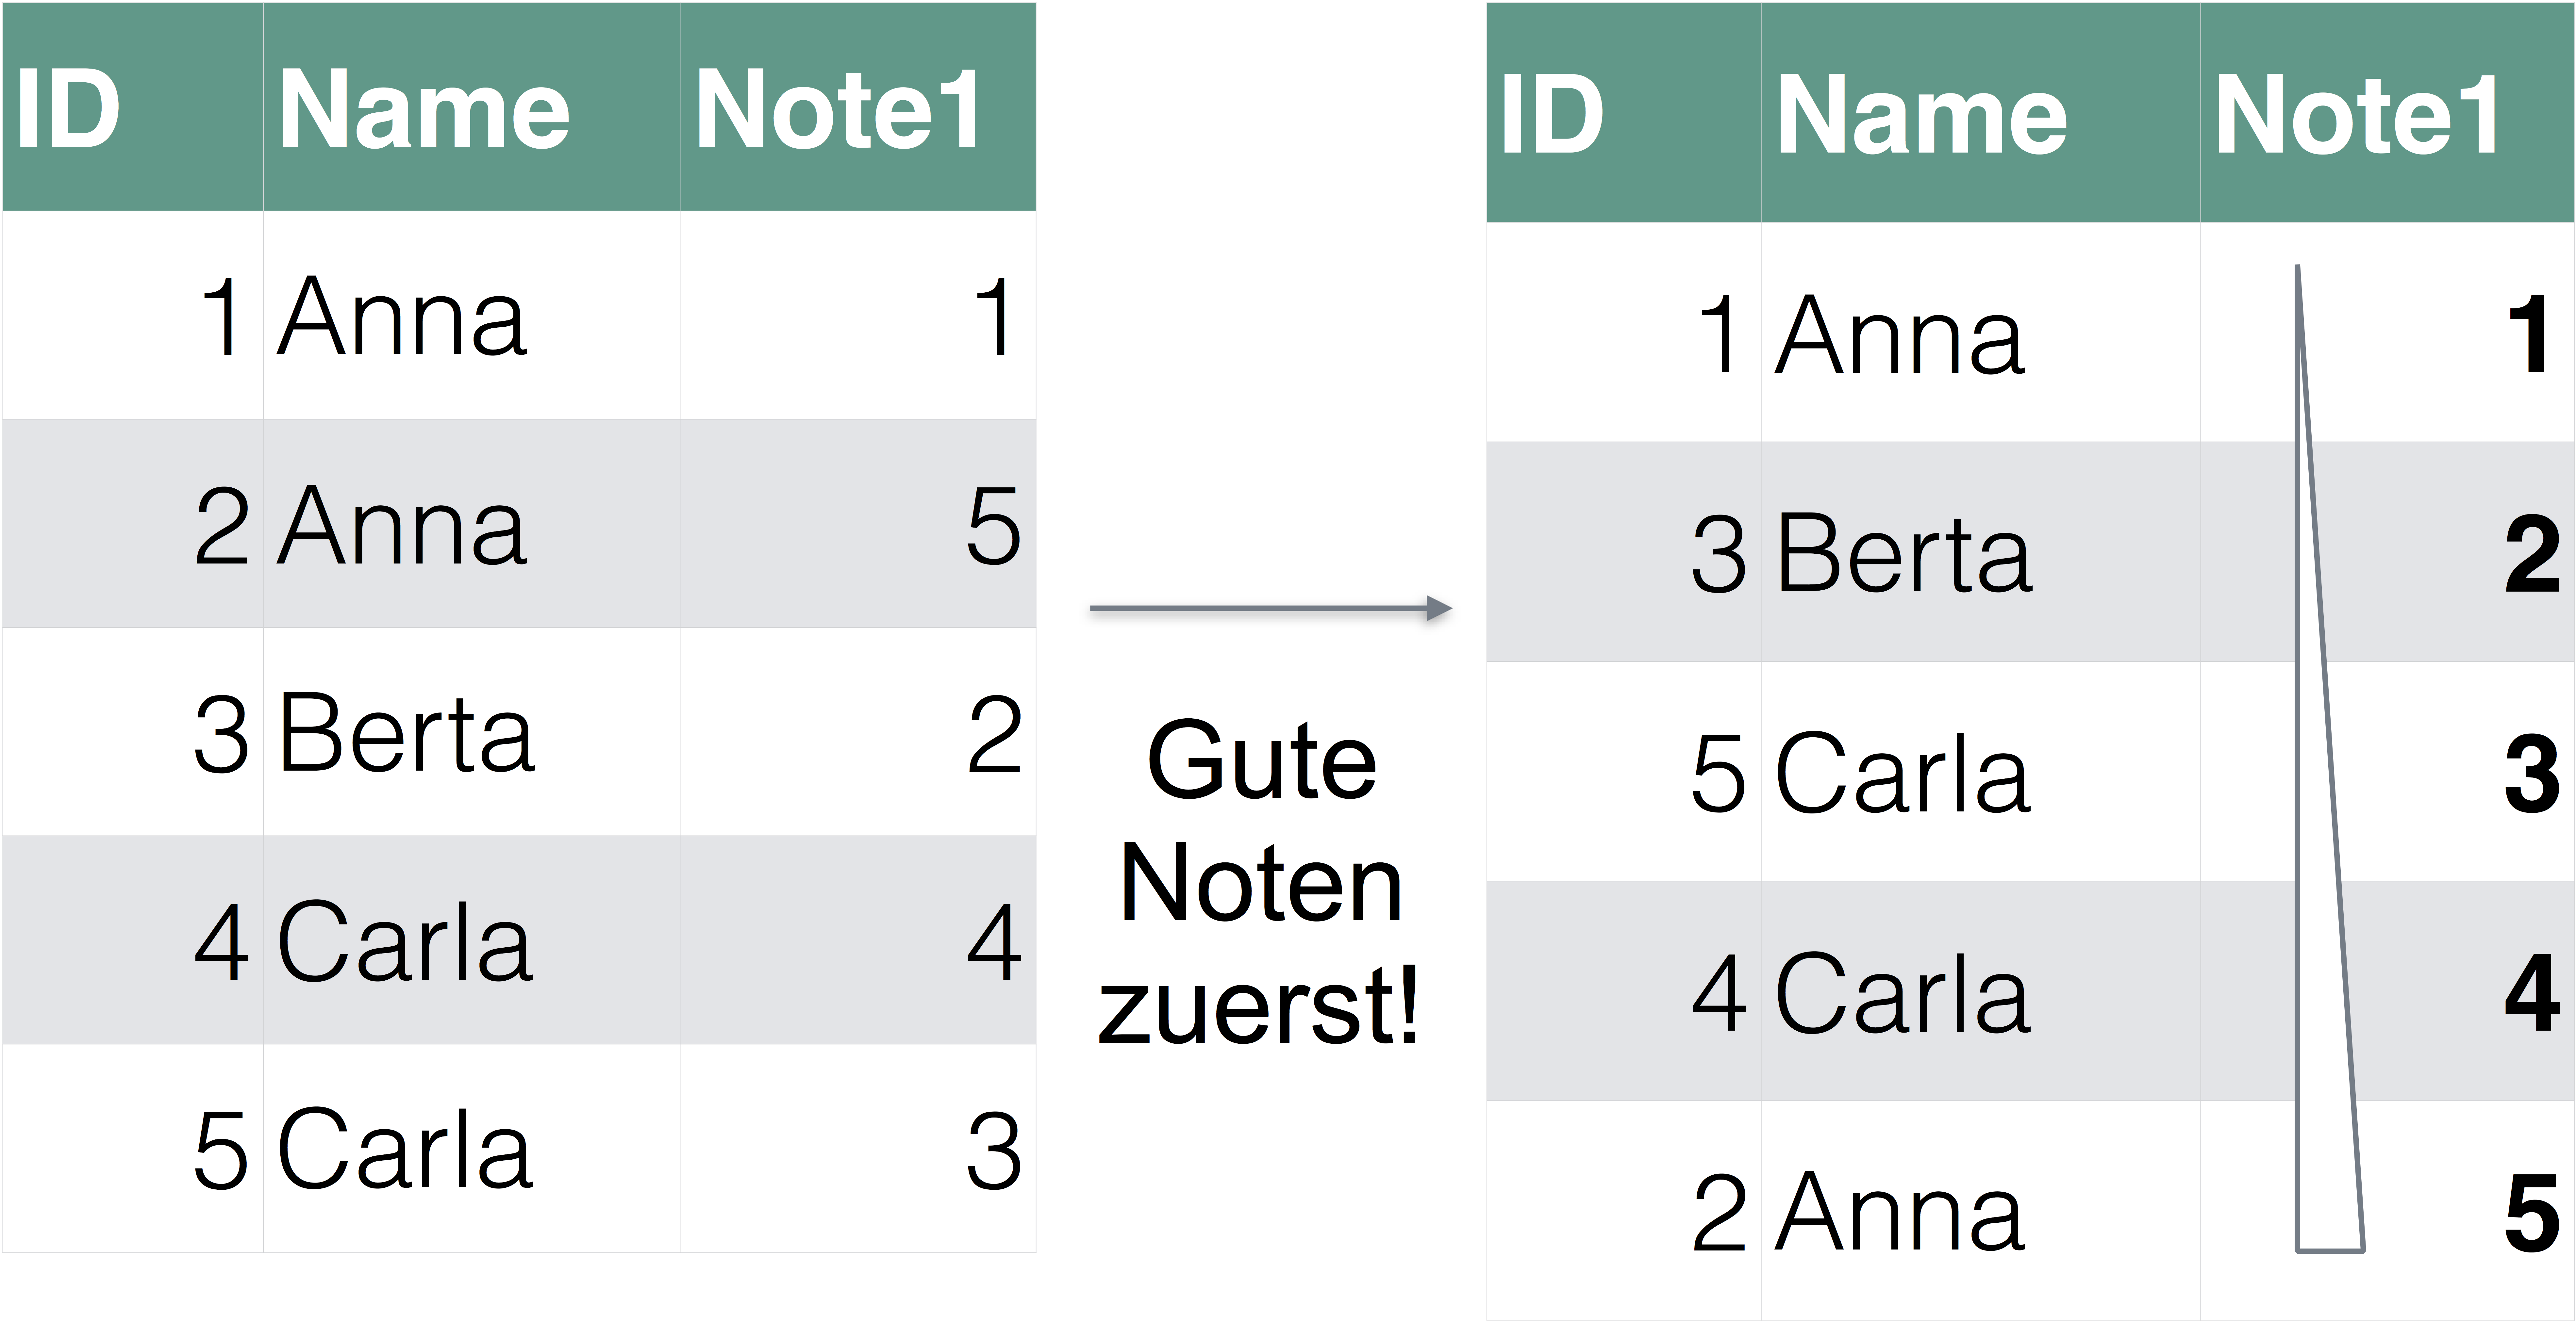
\includegraphics[width=0.8\linewidth]{../images/Datenjudo/arrange-crop} 

}

\caption{Spalten sortieren}\label{fig:fig-arrange}
\end{figure}

\end{frame}

\begin{frame}{Datensatz gruppieren mit \texttt{group\_by}}

\begin{figure}

{\centering 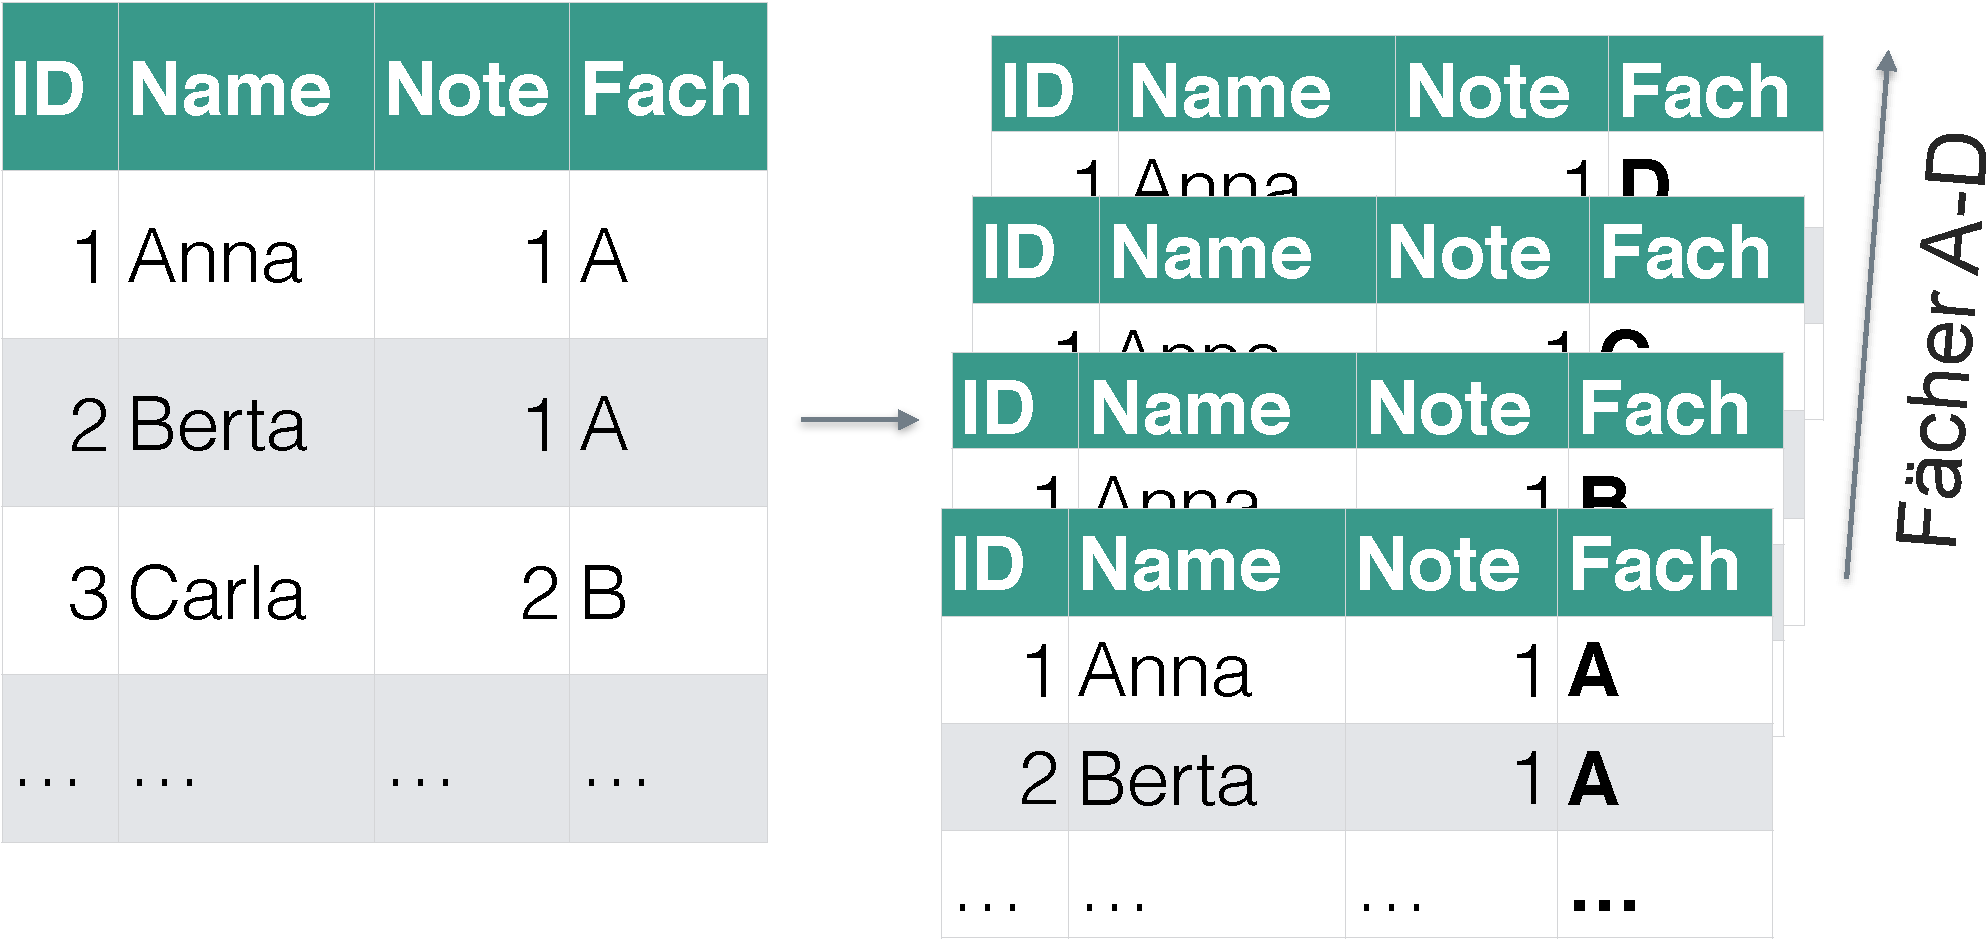
\includegraphics[width=0.8\linewidth]{../images/Datenjudo/group_by} 

}

\caption{Datensätze nach Subgruppen aufteilen}\label{fig:fig-groupby}
\end{figure}

\end{frame}

\begin{frame}{Eine Spalte zusammenfassen mit \texttt{summarise}}

\begin{figure}

{\centering 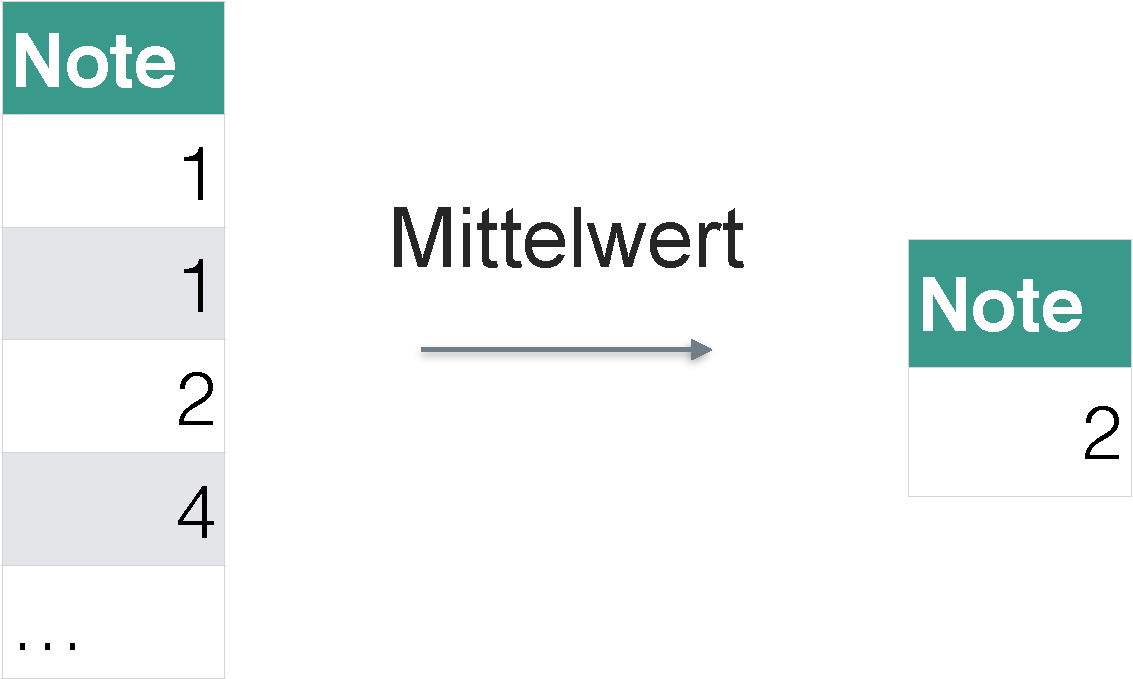
\includegraphics[width=0.8\linewidth]{../images/Datenjudo/summarise} 

}

\caption{Spalten zu einer Zahl zusammenfassen}\label{fig:fig-summarise}
\end{figure}

\end{frame}

\begin{frame}{Zeilen zählen mit \texttt{n} und \texttt{count}}

\begin{figure}

{\centering 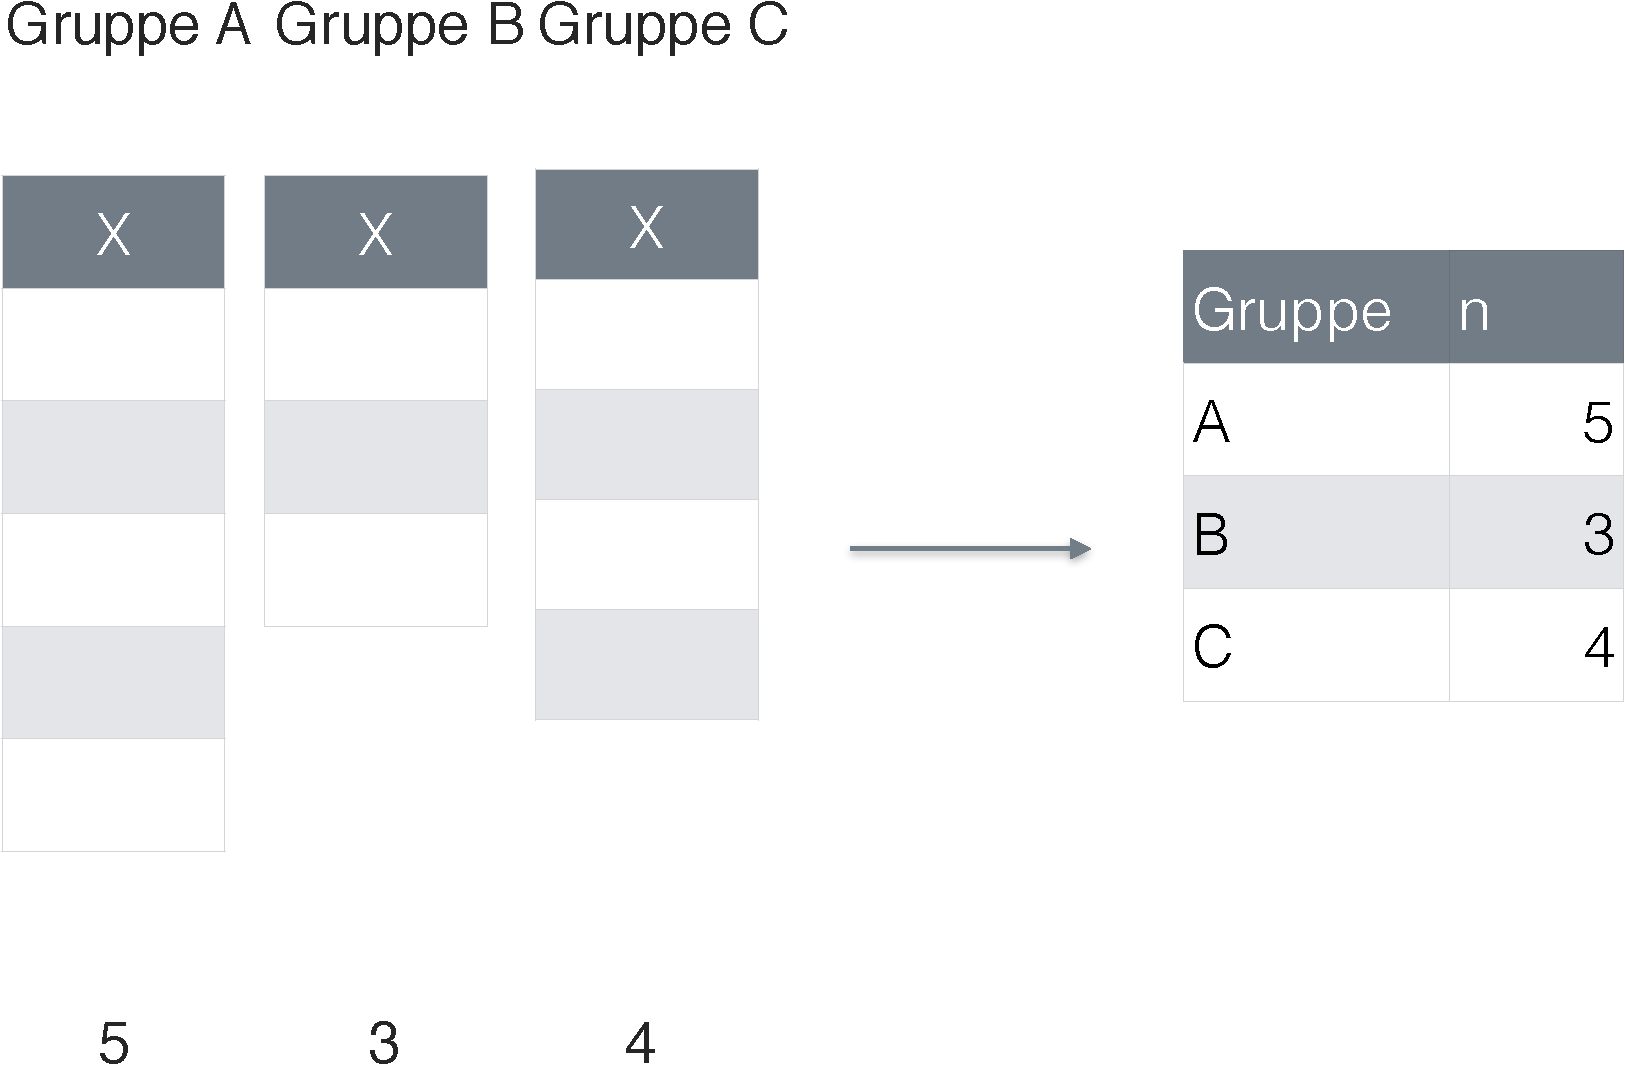
\includegraphics[width=0.8\linewidth]{../images/Datenjudo/count-crop} 

}

\caption{Sinnbild für 'count'}\label{fig:fig-count}
\end{figure}

\end{frame}

\begin{frame}{Die Pfeife}

\begin{figure}

{\centering 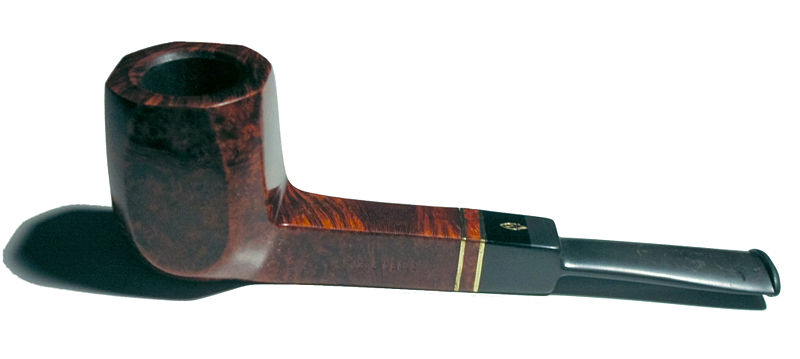
\includegraphics[width=0.8\linewidth]{../images/Datenjudo/800px-Pipa_savinelli} 

}

\caption{Das ist keine Pfeife}\label{fig:cecie-une-pipe}
\end{figure}

\end{frame}

\begin{frame}{Befehle hintereinander reihen mit der Pfeife}

\begin{figure}

{\centering 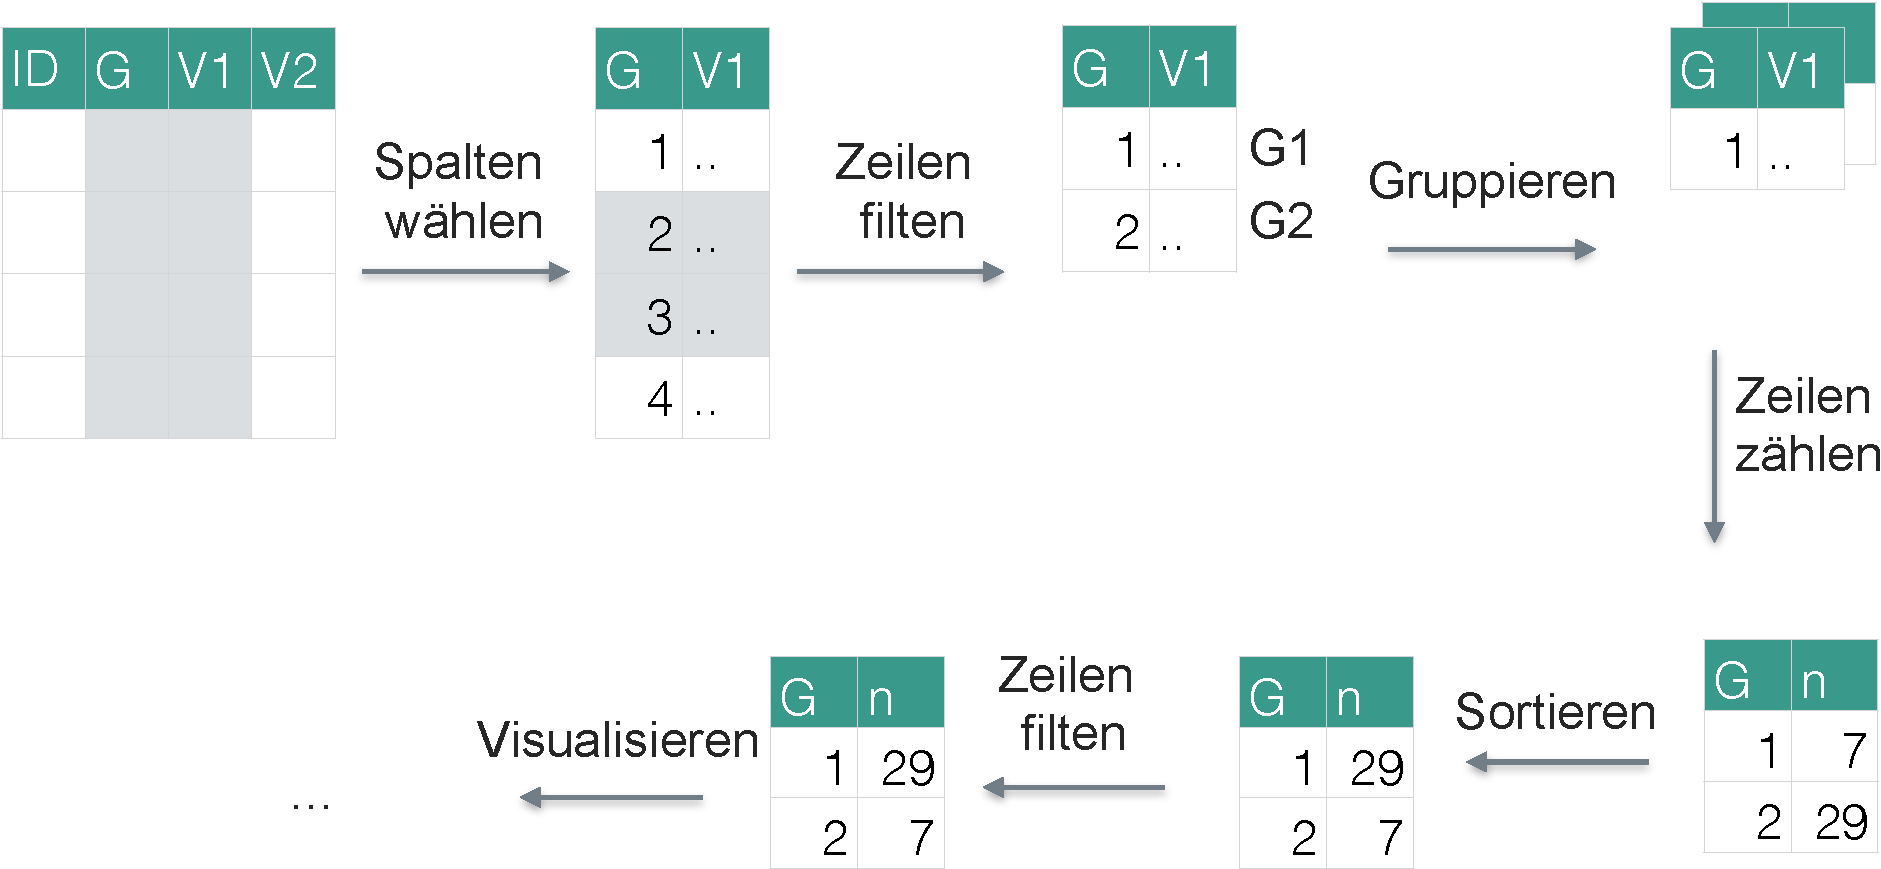
\includegraphics[width=0.8\linewidth]{../images/Datenjudo/durchpfeifen} 

}

\caption{Das 'Durchpeifen'}\label{fig:fig-durchpfeifen}
\end{figure}

\end{frame}

\begin{frame}[fragile]{Introducing Pipe-Syntax}

Vergleichen Sie mal diese Syntax

\begin{Shaded}
\begin{Highlighting}[]
<<<<<<< Updated upstream
\KeywordTok{filter}\NormalTok{(}\KeywordTok{summarise}\NormalTok{(}\KeywordTok{group_by}\NormalTok{(}\KeywordTok{filter}\NormalTok{(stats_test, }\OperatorTok{!}\KeywordTok{is.na}\NormalTok{(score)), interest), }\DataTypeTok{mw =} \KeywordTok{mean}\NormalTok{(score)), }
\NormalTok{    mw }\OperatorTok{>}\StringTok{ }\DecValTok{30}\NormalTok{)}
=======
\KeywordTok{filter}\NormalTok{(}\KeywordTok{summarise}\NormalTok{(}\KeywordTok{group_by}\NormalTok{(}\KeywordTok{filter}\NormalTok{(stats_test, !}\KeywordTok{is.na}\NormalTok{(score)), interest), }\DataTypeTok{mw =} \KeywordTok{mean}\NormalTok{(score)), }
    \NormalTok{mw >}\StringTok{ }\DecValTok{30}\NormalTok{)}
>>>>>>> Stashed changes
\end{Highlighting}
\end{Shaded}

mit dieser

\begin{Shaded}
\begin{Highlighting}[]
<<<<<<< Updated upstream
\NormalTok{stats_test }\OperatorTok\StringTok{ }\KeywordTok{filter}\NormalTok{(}\OperatorTok{!}\KeywordTok{is.na}\NormalTok{(score)) }\OperatorTok\StringTok{ }\KeywordTok{group_by}\NormalTok{(interest) }\OperatorTok\StringTok{ }\KeywordTok{summarise}\NormalTok{(}\DataTypeTok{mw =} \KeywordTok{mean}\NormalTok{(score)) }\OperatorTok\StringTok{ }
\StringTok{    }\KeywordTok{filter}\NormalTok{(mw }\OperatorTok{>}\StringTok{ }\DecValTok{30}\NormalTok{)}
=======
\NormalTok{stats_test %>%}\StringTok{ }\KeywordTok{filter}\NormalTok{(!}\KeywordTok{is.na}\NormalTok{(score)) %>%}\StringTok{ }\KeywordTok{group_by}\NormalTok{(interest) %>%}\StringTok{ }\KeywordTok{summarise}\NormalTok{(}\DataTypeTok{mw =} \KeywordTok{mean}\NormalTok{(score)) %>%}\StringTok{ }
\StringTok{    }\KeywordTok{filter}\NormalTok{(mw >}\StringTok{ }\DecValTok{30}\NormalTok{)}
>>>>>>> Stashed changes
\end{Highlighting}
\end{Shaded}

\end{frame}

\begin{frame}{Pfeifen macht das Leben leichter}

Tipp: In RStudio gibt es einen Shortcut für die Pfeife: Strg-Shift-M
(auf allen Betriebssystemen).

Die Syntax von oben auf Deutsch:

\begin{itemize}
\tightlist
\item
  Nimm die Tabelle ``stats\_test'' UND DANN\\
\item
  filtere alle nicht-fehlenden Werte UND DANN\\
\item
  gruppiere die verbleibenden Werte nach ``interest'' UND DANN\\
\item
  bilde den Mittelwert (pro Gruppe) für ``score'' UND DANN\\
\item
  liefere nur die Werte größer als 30 zurück.
\end{itemize}

\end{frame}

\begin{frame}{Spalten berechnen mit \texttt{mutate}}

\begin{figure}

{\centering 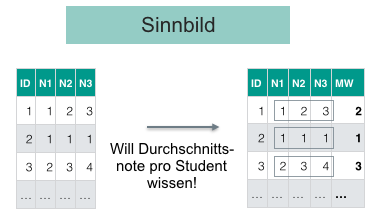
\includegraphics[width=0.8\linewidth]{../images/Datenjudo/mutate} 

}

\caption{Sinnbild für mutate}\label{fig:fig-mutate}
\end{figure}

\end{frame}

\begin{frame}[fragile]{Beispiel für \texttt{mutate}}

\begin{Shaded}
\begin{Highlighting}[]
<<<<<<< Updated upstream
\NormalTok{stats_test }\OperatorTok\StringTok{ }\KeywordTok{mutate}\NormalTok{(}\DataTypeTok{Streber =}\NormalTok{ score }\OperatorTok{>}\StringTok{ }\DecValTok{38}\NormalTok{) }\OperatorTok\StringTok{ }\KeywordTok{head}\NormalTok{()}
=======
\NormalTok{stats_test %>%}\StringTok{ }\KeywordTok{mutate}\NormalTok{(}\DataTypeTok{Streber =} \NormalTok{score >}\StringTok{ }\DecValTok{38}\NormalTok{) %>%}\StringTok{ }\KeywordTok{head}\NormalTok{()}
>>>>>>> Stashed changes
\end{Highlighting}
\end{Shaded}

\end{frame}

\begin{frame}[fragile]{Deskriptive Statistik mit \texttt{dplyr}}

\begin{Shaded}
\begin{Highlighting}[]
<<<<<<< Updated upstream
\NormalTok{stats_test2 <-}\StringTok{ }\KeywordTok{select}\NormalTok{(stats_test, }\OperatorTok{-}\NormalTok{date_time)}
=======
\NormalTok{stats_test2 <-}\StringTok{ }\KeywordTok{select}\NormalTok{(stats_test, -date_time)}
>>>>>>> Stashed changes
\KeywordTok{desctable}\NormalTok{(stats_test2l)}
\end{Highlighting}
\end{Shaded}

\end{frame}

\section{Daten visualisieren}\label{vis}

\begin{frame}{Lernziele für das Kapitel `Daten visualisieren'}

\begin{itemize}
\tightlist
\item
  An einem Beispiel erläutern können, warum/ wann ein Bild mehr sagt,
  als 1000 Worte.
\item
  Häufige Arten von Diagrammen erstellen können.
\item
  Diagramme bestimmten Zwecken zuordnen können.
\end{itemize}

\end{frame}

\begin{frame}{Statistik ist wie ein Bikini\ldots{}}

\begin{figure}

{\centering 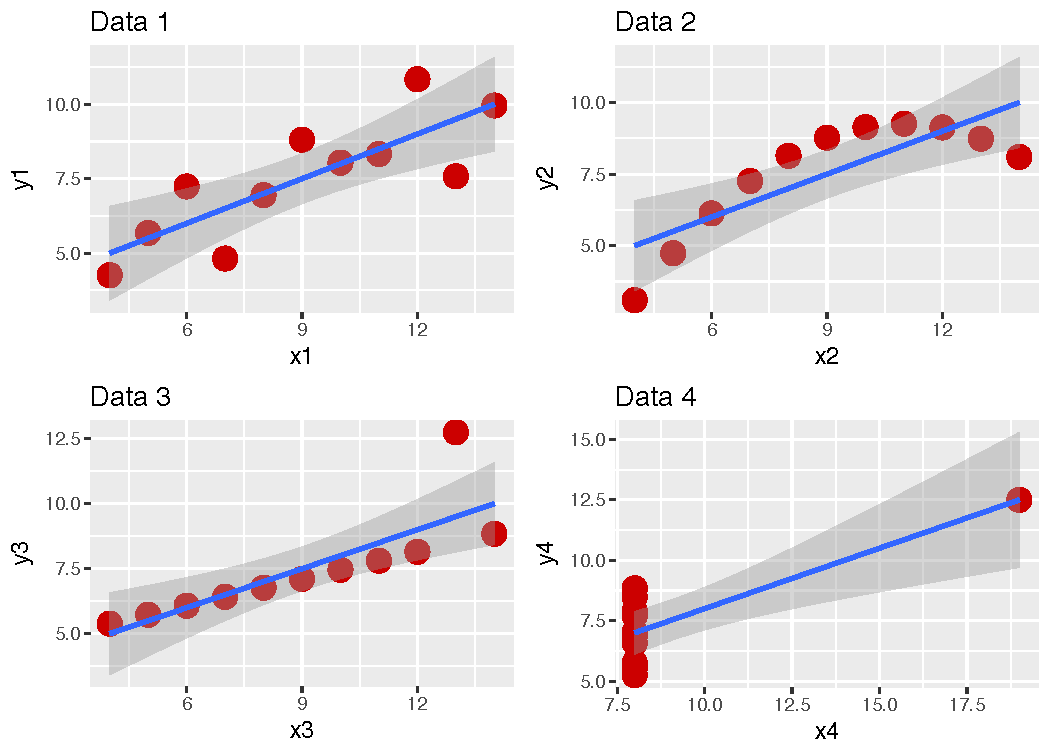
\includegraphics[width=0.5\linewidth]{../images/visualisieren/anscombe} 

}

\caption{Das Anscombe-Quartett}\label{fig:fig-anscombe}
\end{figure}

\href{https://youtu.be/DbJyPELmhJc}{Dinosaurier-Video}

\end{frame}

\begin{frame}{Die Anatomie eines Diagramms}

\begin{figure}

{\centering 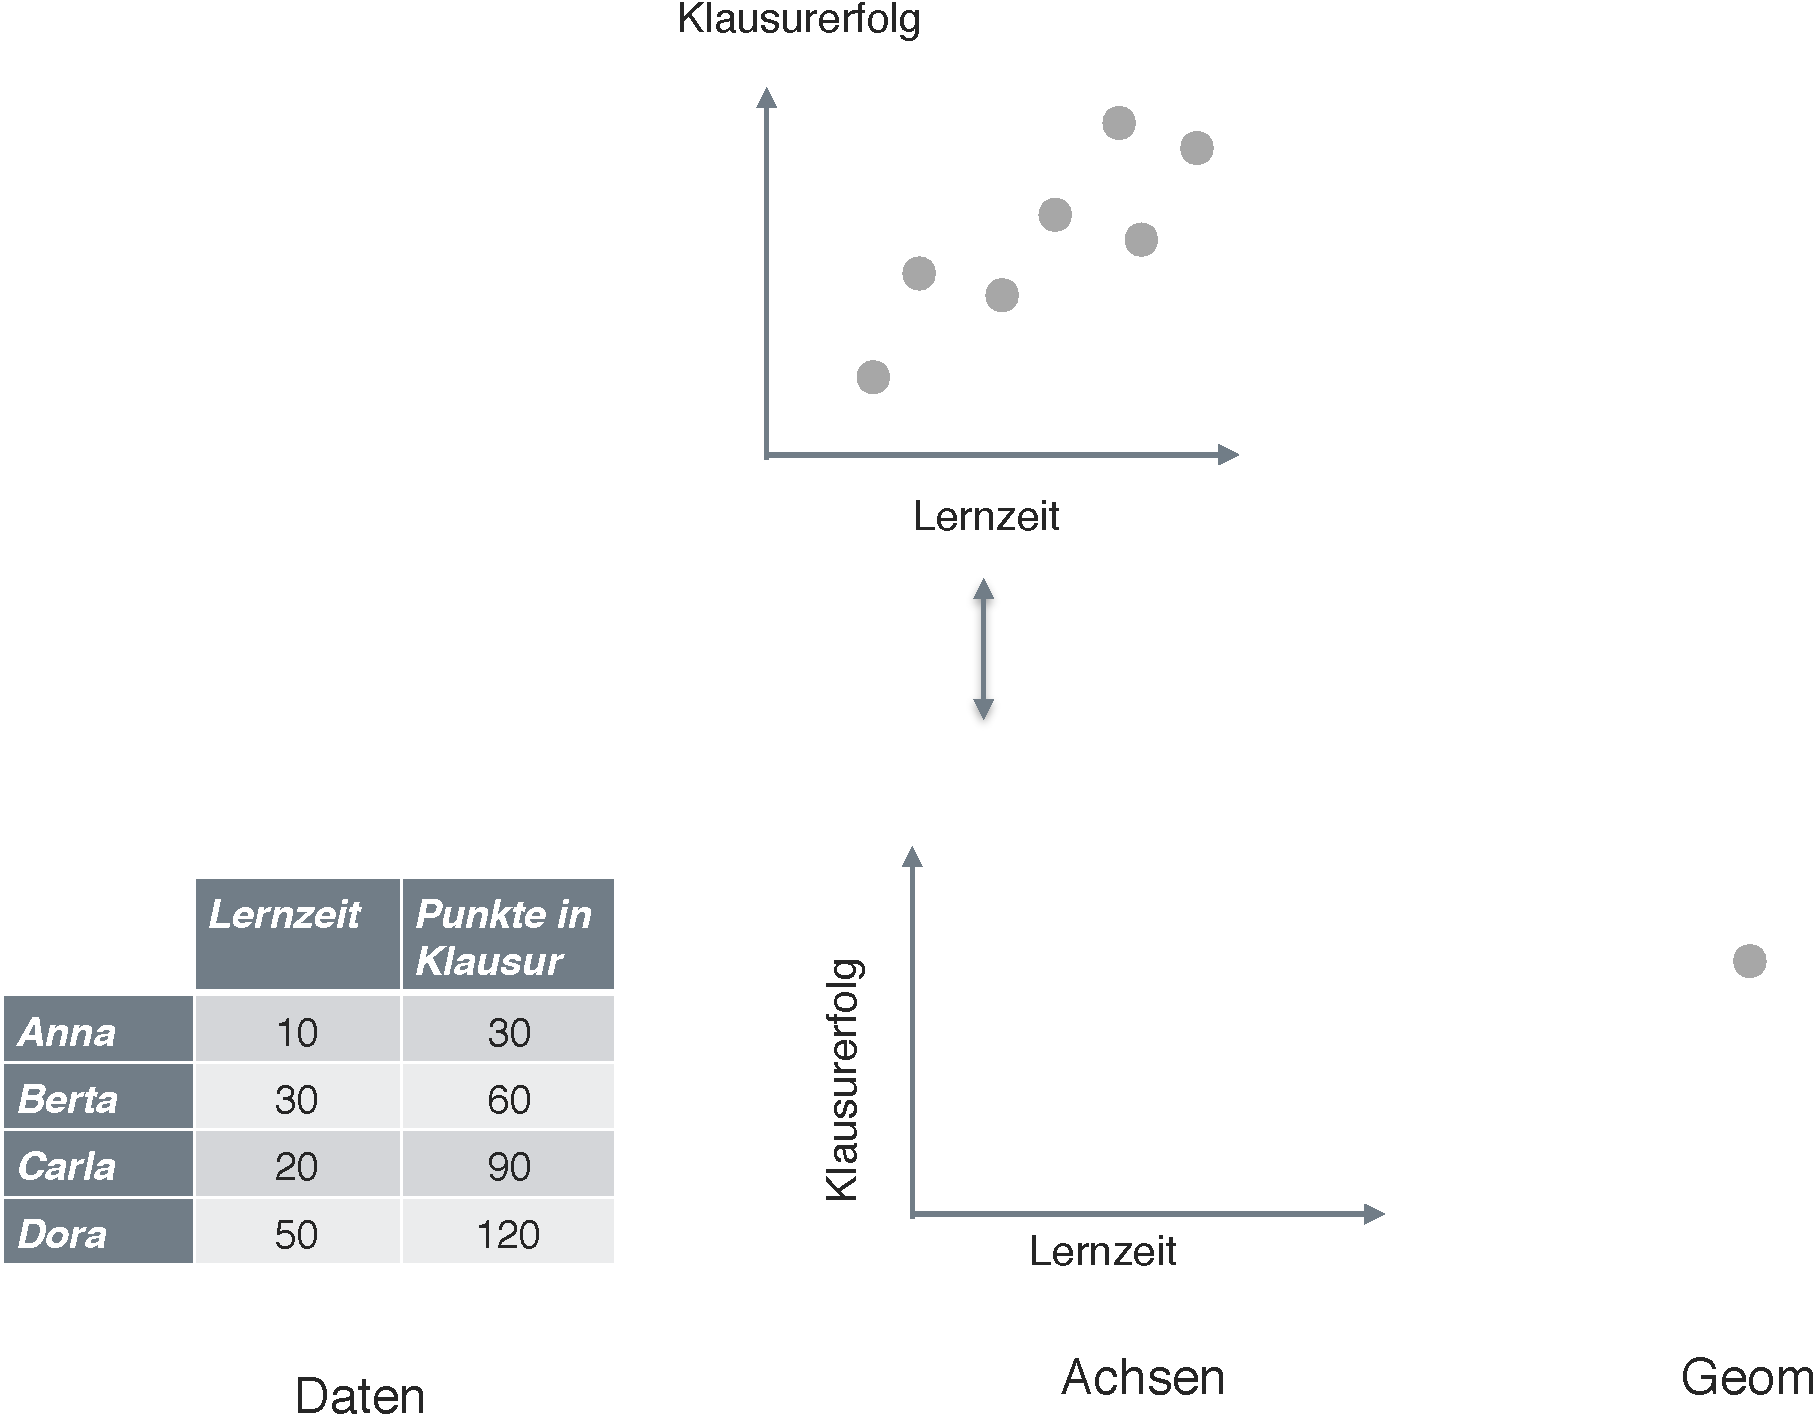
\includegraphics[width=0.5\linewidth]{../images/visualisieren/anatomie_diagramm_crop} 

}

\caption{Anatomie eines Diagramms}\label{fig:fig-anatomie}
\end{figure}

\end{frame}

\begin{frame}[fragile]{Beispiel für ein Diagramm it mit
\texttt{ggplot2::qplot}}

\begin{Shaded}
\begin{Highlighting}[]
<<<<<<< Updated upstream
\KeywordTok{qplot}\NormalTok{(}\DataTypeTok{x =}\NormalTok{ year, }\DataTypeTok{y =}\NormalTok{ budget, }\DataTypeTok{geom =} \StringTok{"point"}\NormalTok{, }\DataTypeTok{data =}\NormalTok{ movies)}
=======
\KeywordTok{qplot}\NormalTok{(}\DataTypeTok{x =} \NormalTok{year, }\DataTypeTok{y =} \NormalTok{budget, }\DataTypeTok{geom =} \StringTok{"point"}\NormalTok{, }\DataTypeTok{data =} \NormalTok{movies)}
>>>>>>> Stashed changes
\end{Highlighting}
\end{Shaded}

\begin{figure}

{\centering 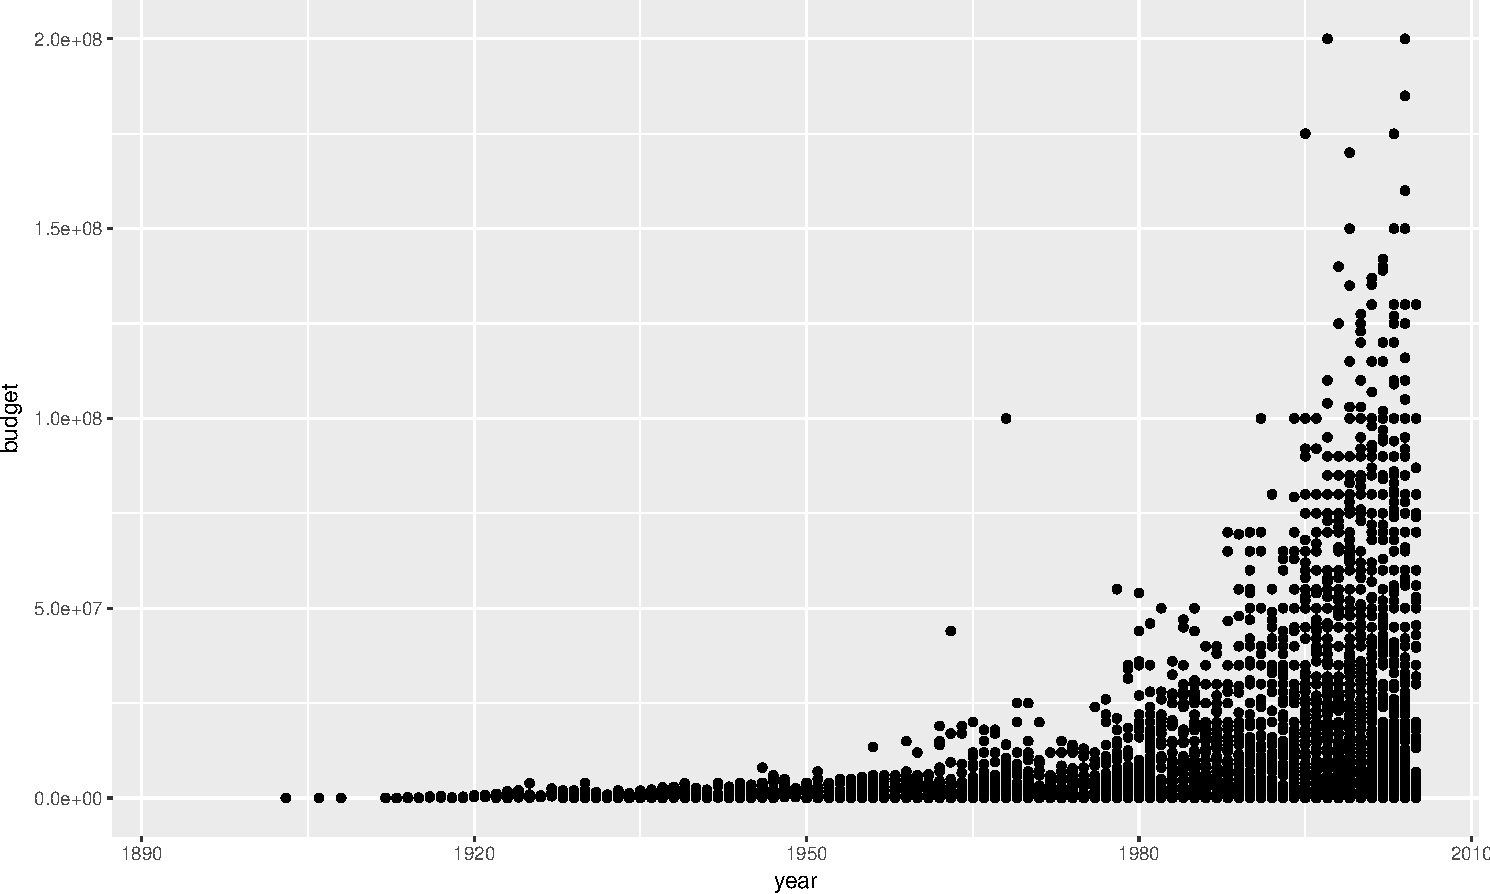
\includegraphics[width=0.5\linewidth]{PraDa_Folien_nm_2_files/figure-beamer/fig-movies-1} 

}

\caption{Mittleres Budget pro Jahr}\label{fig:fig-movies}
\end{figure}

\end{frame}

\begin{frame}[fragile]{Anatomiestunde mit \texttt{qplot}}

\begin{itemize}
\tightlist
\item
  \texttt{qplot}: Erstelle schnell (q wie quick in \texttt{qplot}) mal
  einen Plot (engl. ``plot'': Diagramm).\\
\item
  \texttt{x}: Der X-Achse soll die Variable ``year'' zugeordnet
  werden.\\
\item
  \texttt{y}: Der Y-Achse soll die Variable ``budget'' zugeorndet
  werden.\\
\item
  \texttt{geom}: (``geometriches Objekt'') Gemalt werden sollen Punkte
  und zwar pro Beobachtung (hier: Film) ein Punkt; nicht etwa Linien
  oder Boxplots.
\item
  \texttt{data}: Als Datensatz bitte \texttt{movies} verwenden.
\end{itemize}

\end{frame}

\begin{frame}[fragile]{Syntax-Blaupause für \texttt{qplot}}

Diese Syntax des letzten Beispiels ist recht einfach, nämlich:

\begin{Shaded}
\begin{Highlighting}[]
<<<<<<< Updated upstream
\KeywordTok{qplot}\NormalTok{(}\DataTypeTok{x =}\NormalTok{ X_Achse, }\DataTypeTok{y =}\NormalTok{ Y_Achse, }\DataTypeTok{data =}\NormalTok{ mein_dataframe, }\DataTypeTok{geom =} \StringTok{"ein_geom"}\NormalTok{)}
=======
\KeywordTok{qplot}\NormalTok{(}\DataTypeTok{x =} \NormalTok{X_Achse, }\DataTypeTok{y =} \NormalTok{Y_Achse, }\DataTypeTok{data =} \NormalTok{mein_dataframe, }\DataTypeTok{geom =} \StringTok{"ein_geom"}\NormalTok{)}
>>>>>>> Stashed changes
\end{Highlighting}
\end{Shaded}

\end{frame}

\begin{frame}{Häufige Diagrammtypen}

\href{https://sebastiansauer.github.io/Praxis_der_Datenanalyse/daten-visualisieren.html\#haufige-arten-von-diagrammen}{s.
Skript}

\begin{itemize}
\tightlist
\item
  Histogramm, Dichtediagramm
\item
  Punkte, Schachbrett-Diagramme
\item
  Balkendiagramm
\item
  Mosaicplot (Fliesendiagramm)
\item
  Punktediagramm für Zusammenfassungen
\item
  Boxplots
\end{itemize}

\end{frame}

\section{Grundlagen des Modellierens}\label{mod}

\begin{frame}{Prozess der Datenanalyse - Modellieren}

\begin{center}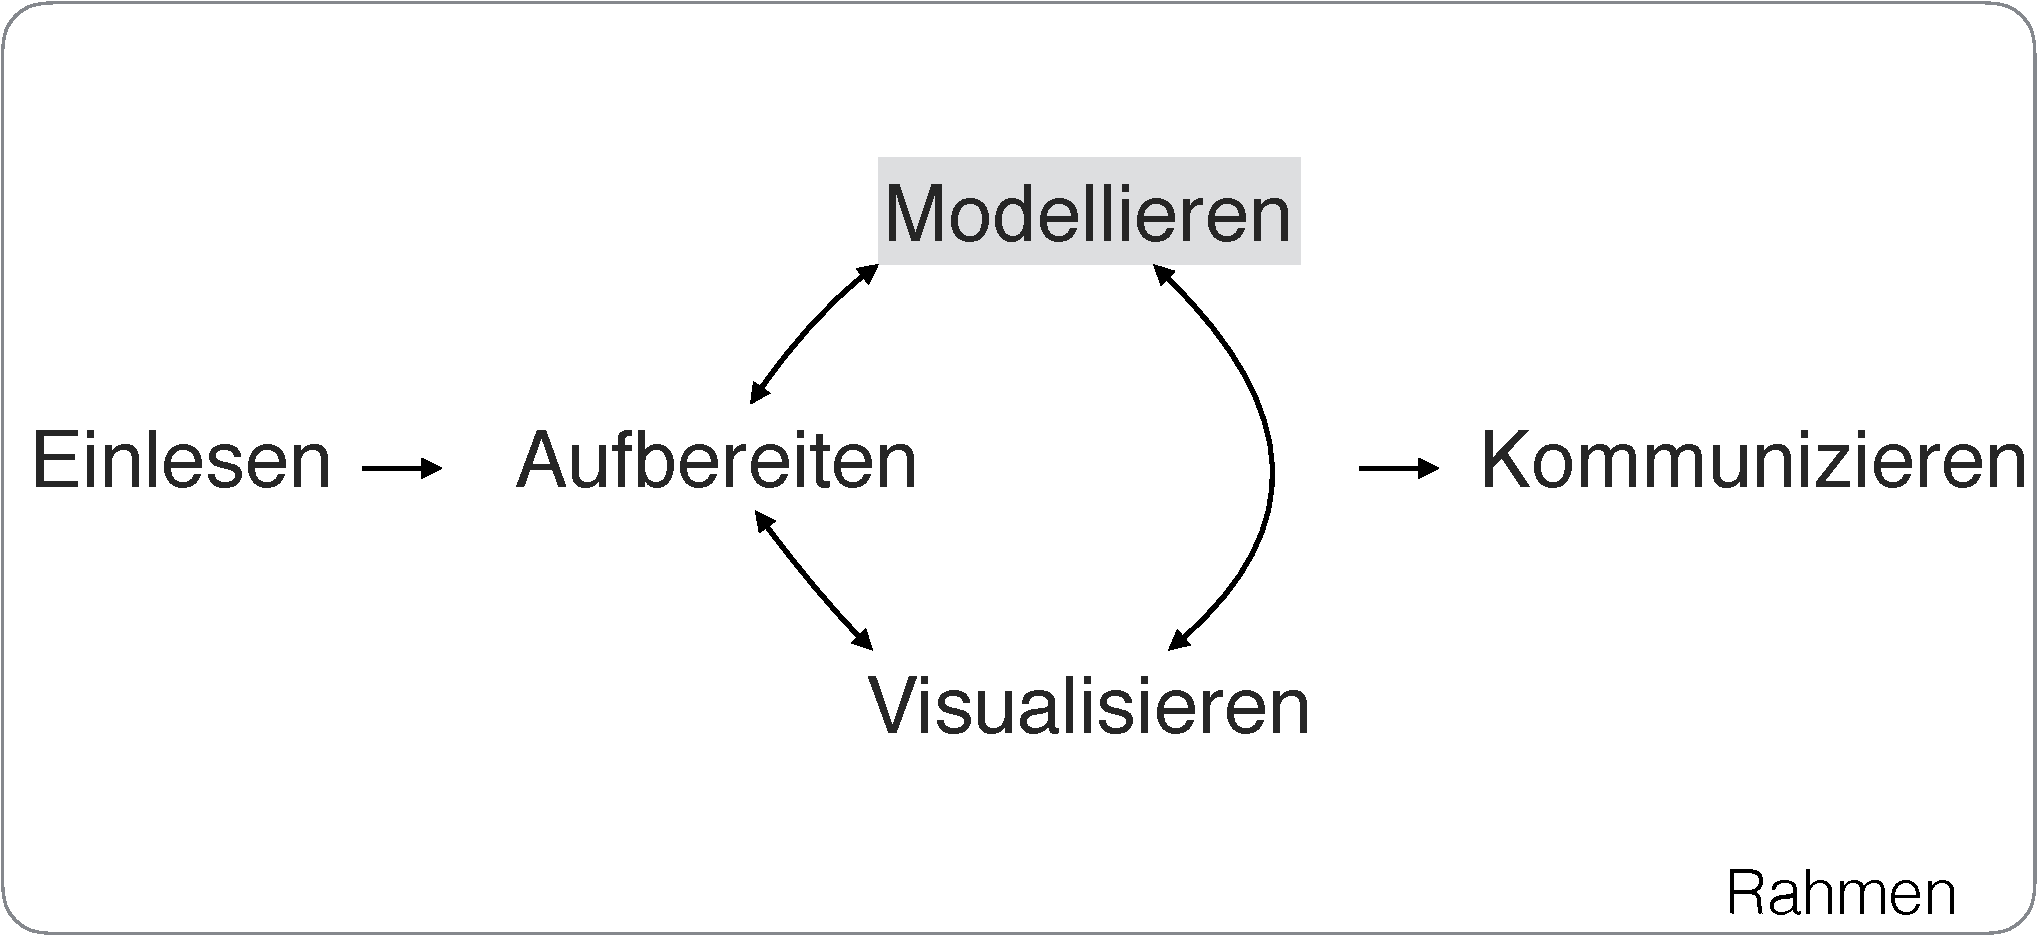
\includegraphics[width=0.7\linewidth]{../images/modellieren/Modellieren} \end{center}

\end{frame}

\begin{frame}{Was ist ein Modell}

\begin{figure}

{\centering 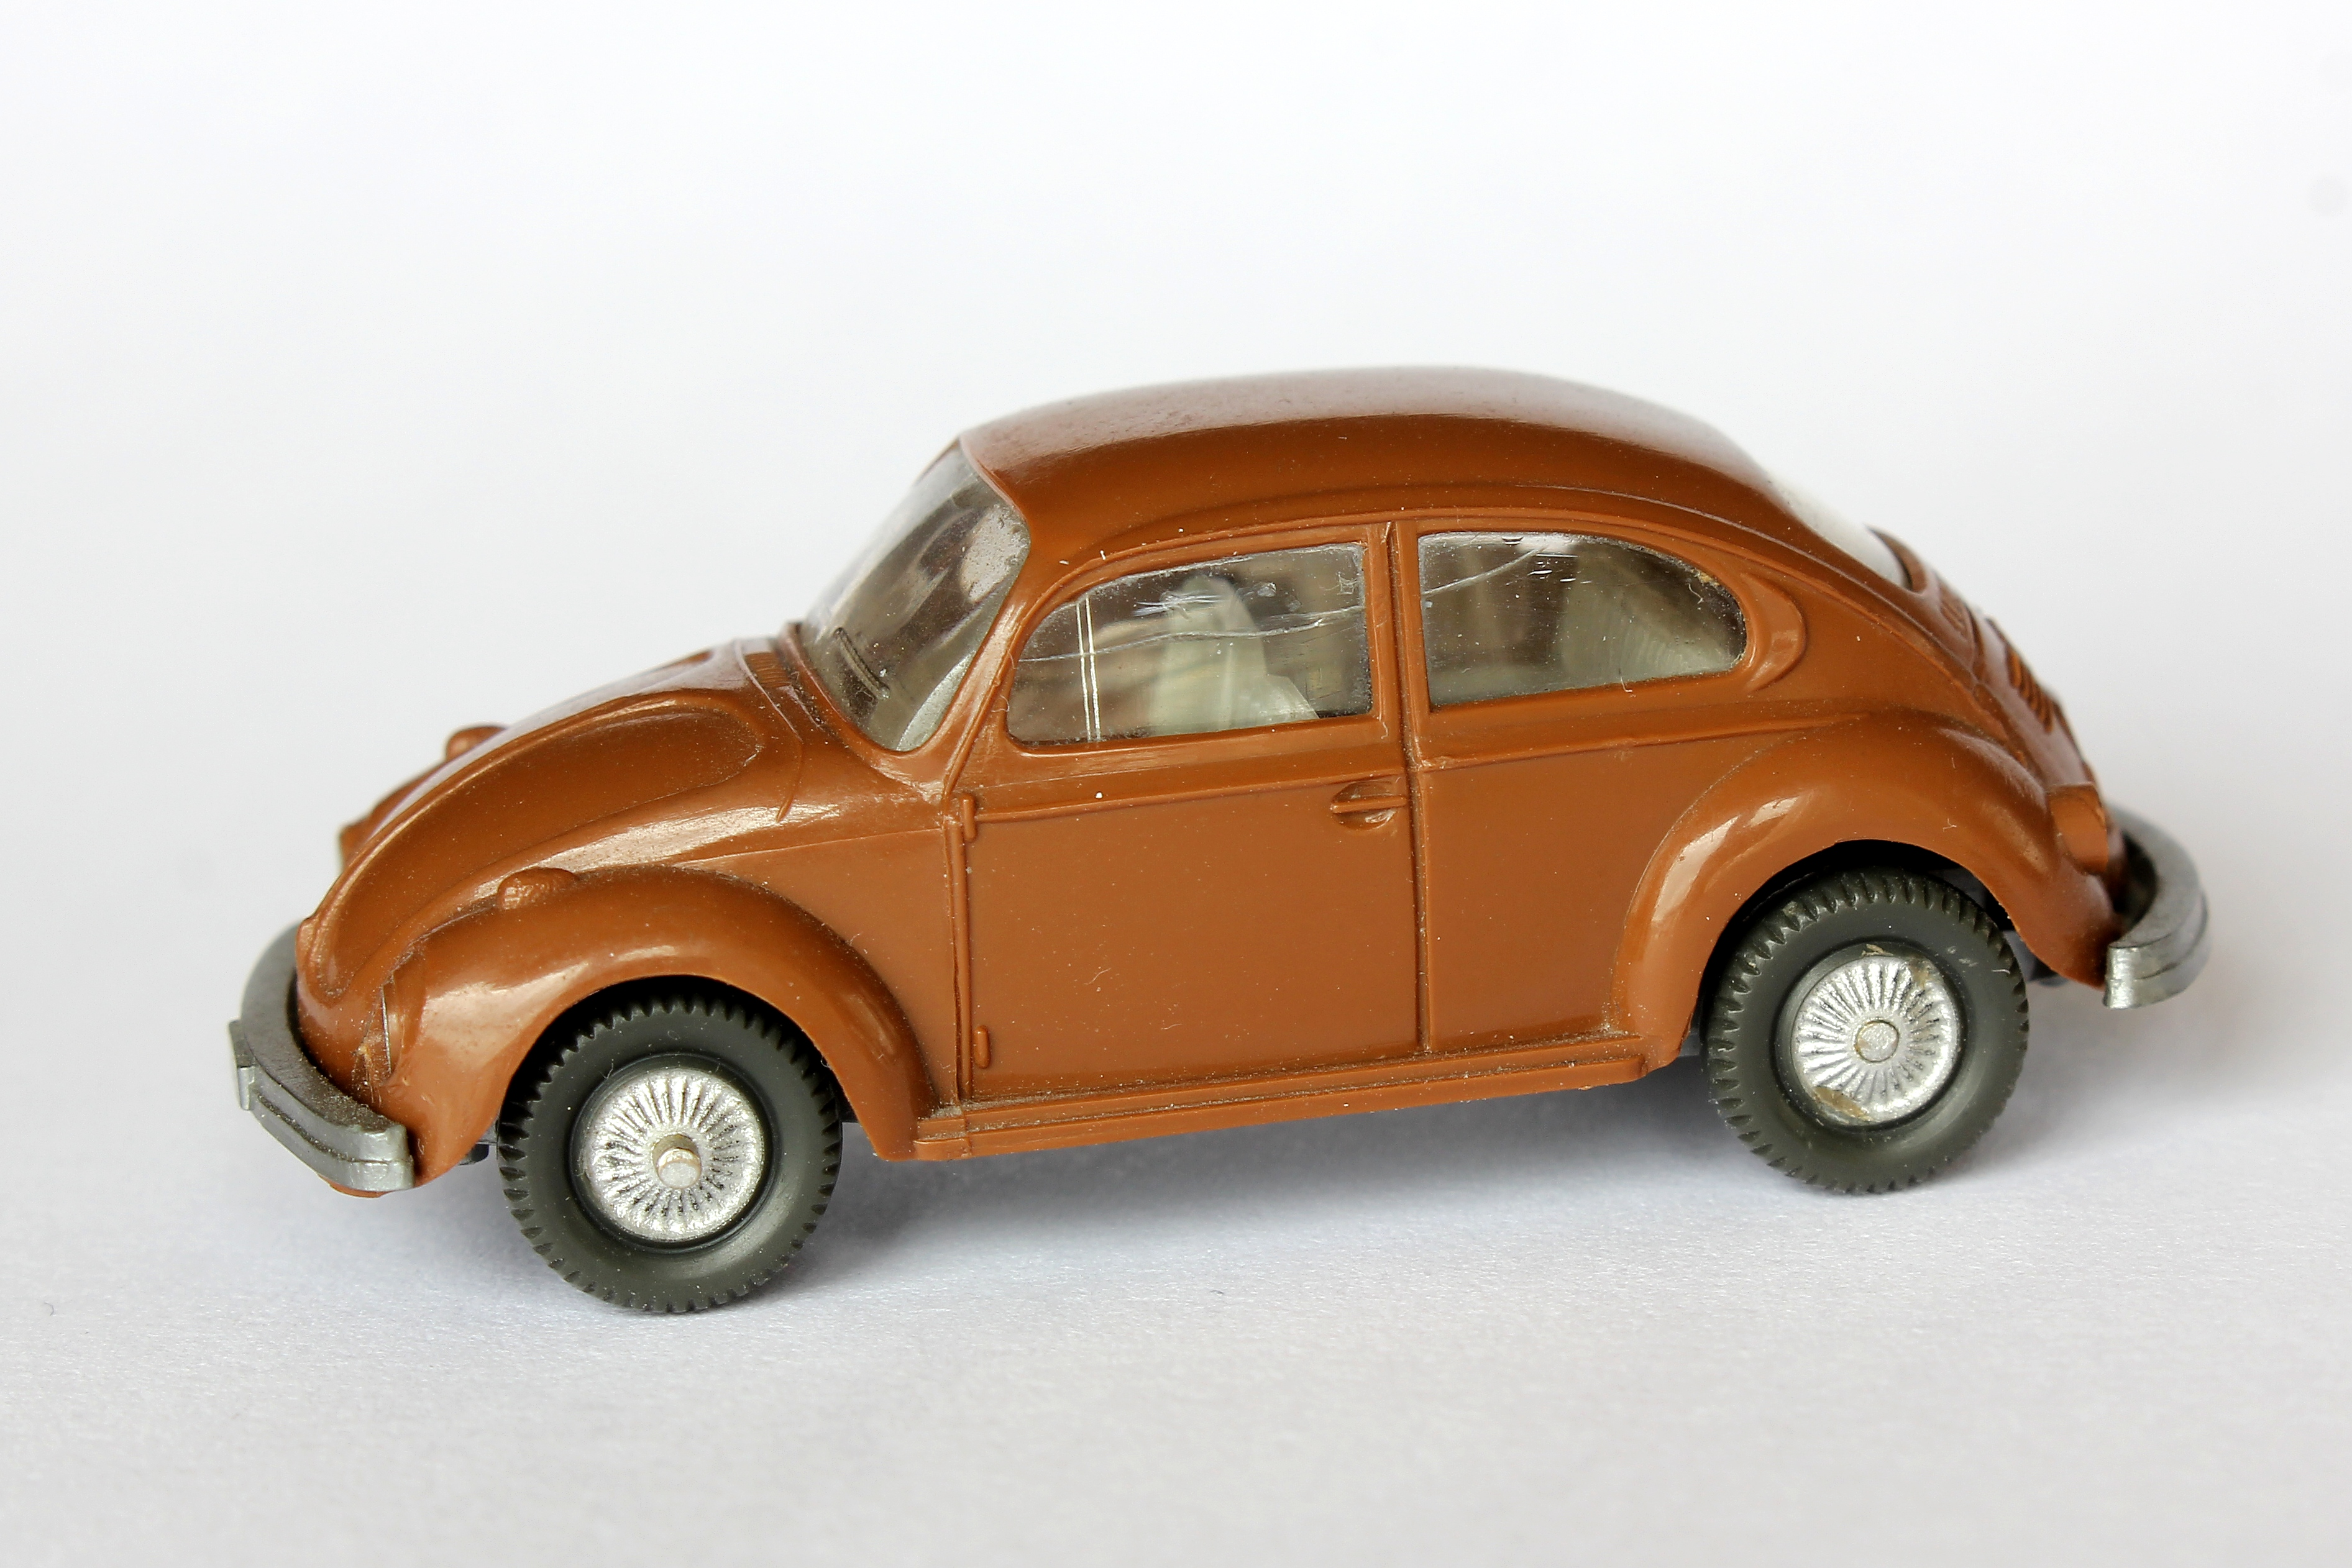
\includegraphics[width=0.8\linewidth]{../images/modellieren/vw_modell} 

}

\caption{Modell eines VW-Käfers}\label{fig:vwmodell}
\end{figure}

\end{frame}

\begin{frame}{Die Beziehung von Gegenstandsbereich und Modell}

\begin{figure}

{\centering 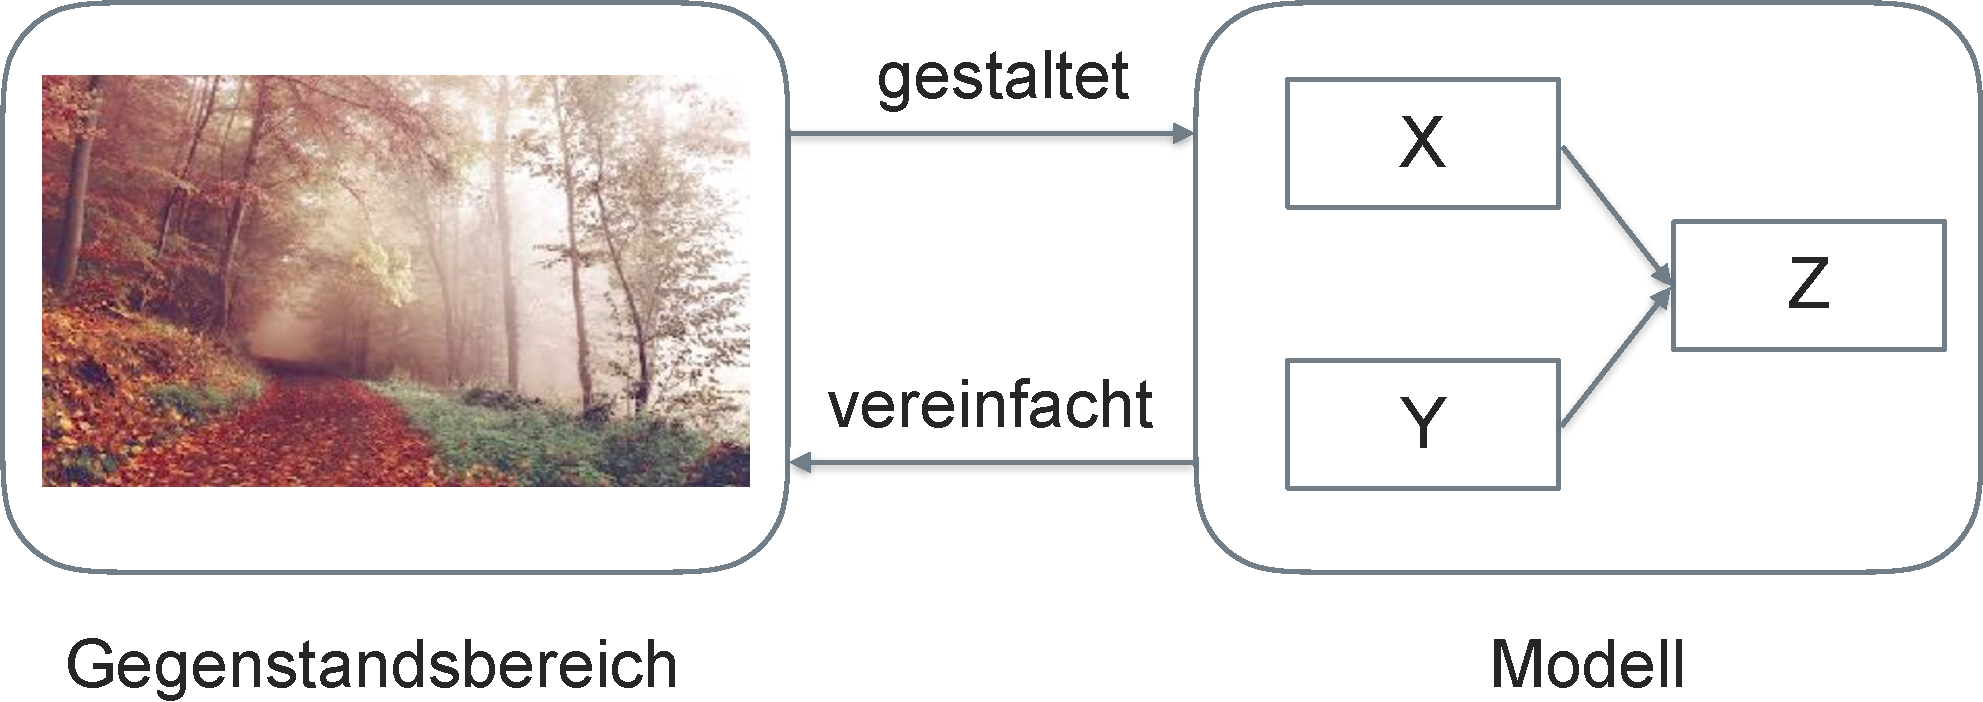
\includegraphics[width=0.8\linewidth]{../images/modellieren/Modell} 

}

\caption{Modellieren}\label{fig:modellieren-plot}
\end{figure}

\end{frame}

\begin{frame}{Modelle spiegeln empirische Relationen in numerischen
Relationen}

\begin{quote}
Modellieren bedeutet ein Verfahren zu erstellen, welches empirische
Sachverhalte adäquat in numerische Sachverhalte umsetzt.
\end{quote}

\begin{figure}

{\centering 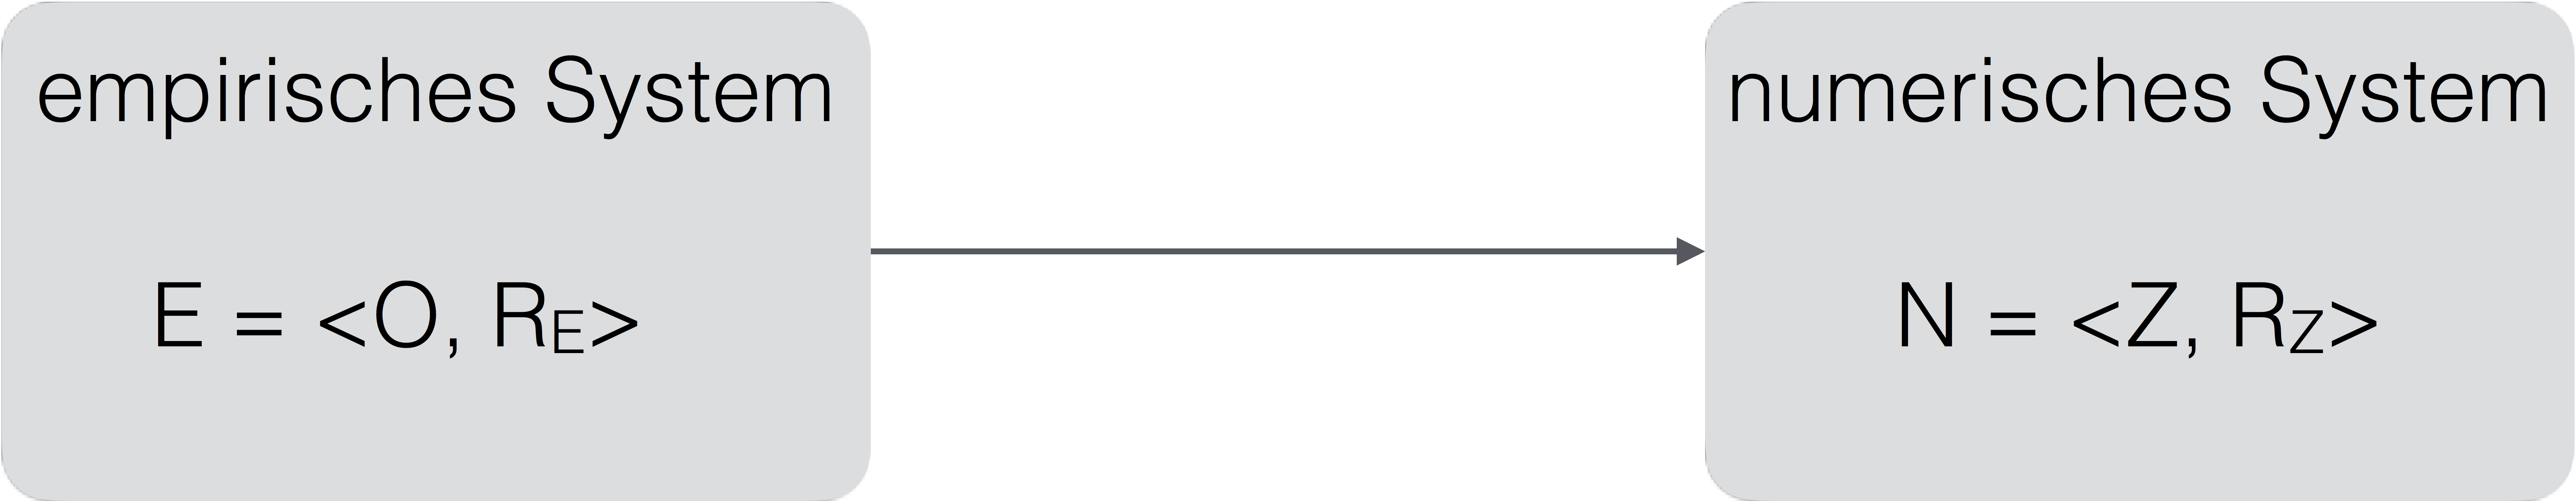
\includegraphics[width=0.8\linewidth]{../images/modellieren/Modellieren_formal_crop} 

}

\caption{Formaleres Modell des Modellierens}\label{fig:modellieren-formal}
\end{figure}

\end{frame}

\begin{frame}{Ein Beispiel zum Modellieren aus der Datenanalyse}

\begin{center}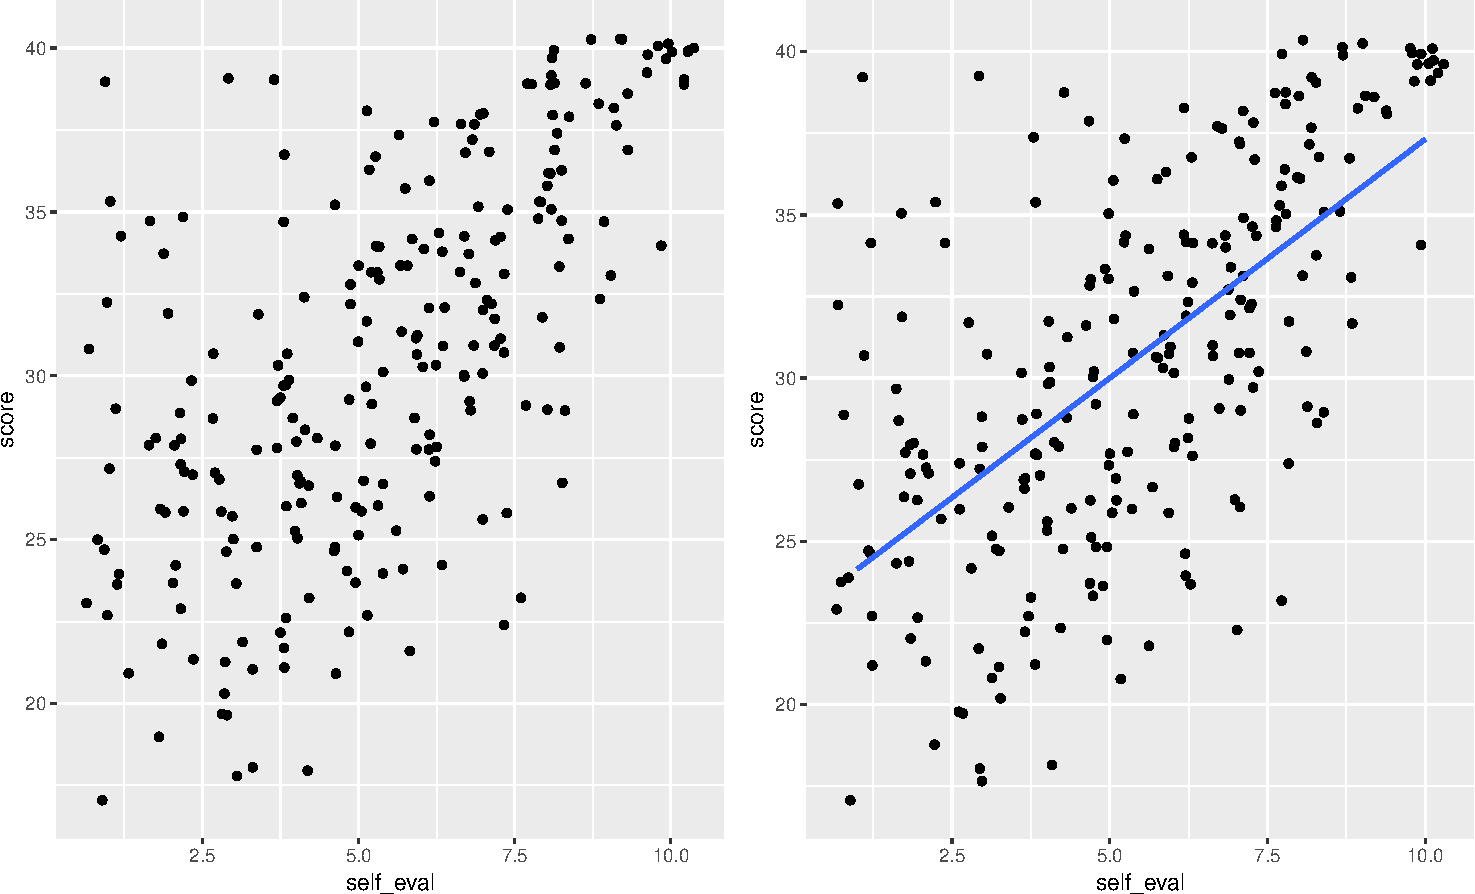
\includegraphics[width=0.8\linewidth]{PraDa_Folien_nm_2_files/figure-beamer/plot-stats-smooth-1} \end{center}

Die blaue Gerade ist ein Modell für den Datensatz (sie versucht es
zumindest).

\end{frame}

\begin{frame}{Modelle umfassen drei Aspekte}

\begin{figure}

{\centering 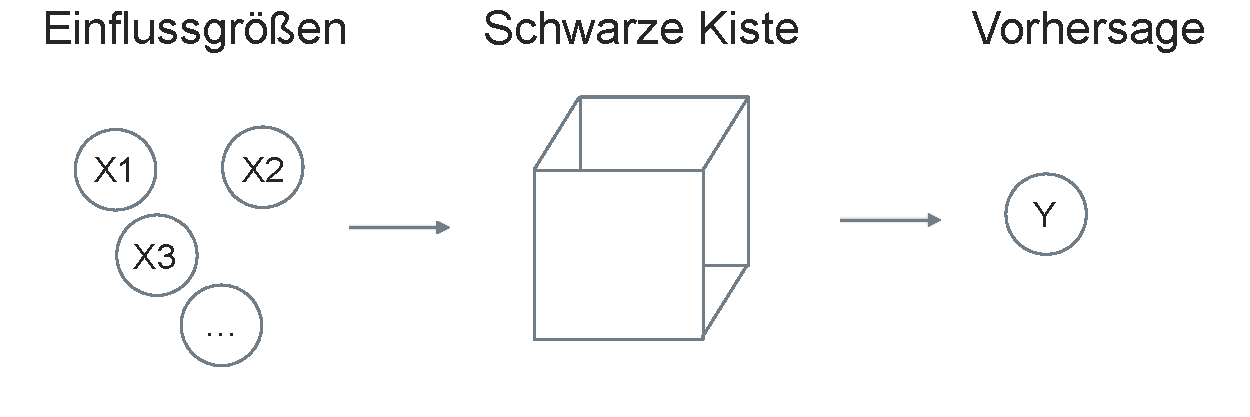
\includegraphics[width=0.8\linewidth]{../images/modellieren/Modell_Blackbox} 

}

\caption{Modelle mit schwarzer Kiste}\label{fig:fig-blackbox}
\end{figure}

\end{frame}

\begin{frame}{Taxonomie der Ziele des Modellierens}

\begin{itemize}
\tightlist
\item
  Geleitetes Modellieren

  \begin{itemize}
  \tightlist
  \item
    Prädiktives Modellieren
  \item
    Explikaties Modellieren
  \end{itemize}
\item
  Ungeleitetes Modellieren

  \begin{itemize}
  \tightlist
  \item
    Dimensionsreduzierendes Modellieren
  \item
    Fallreduzierendes Modellieren
  \end{itemize}
\end{itemize}

\end{frame}

\begin{frame}{Veranschaulichung der beiden Arten des Modellierens}

\begin{figure}

{\centering 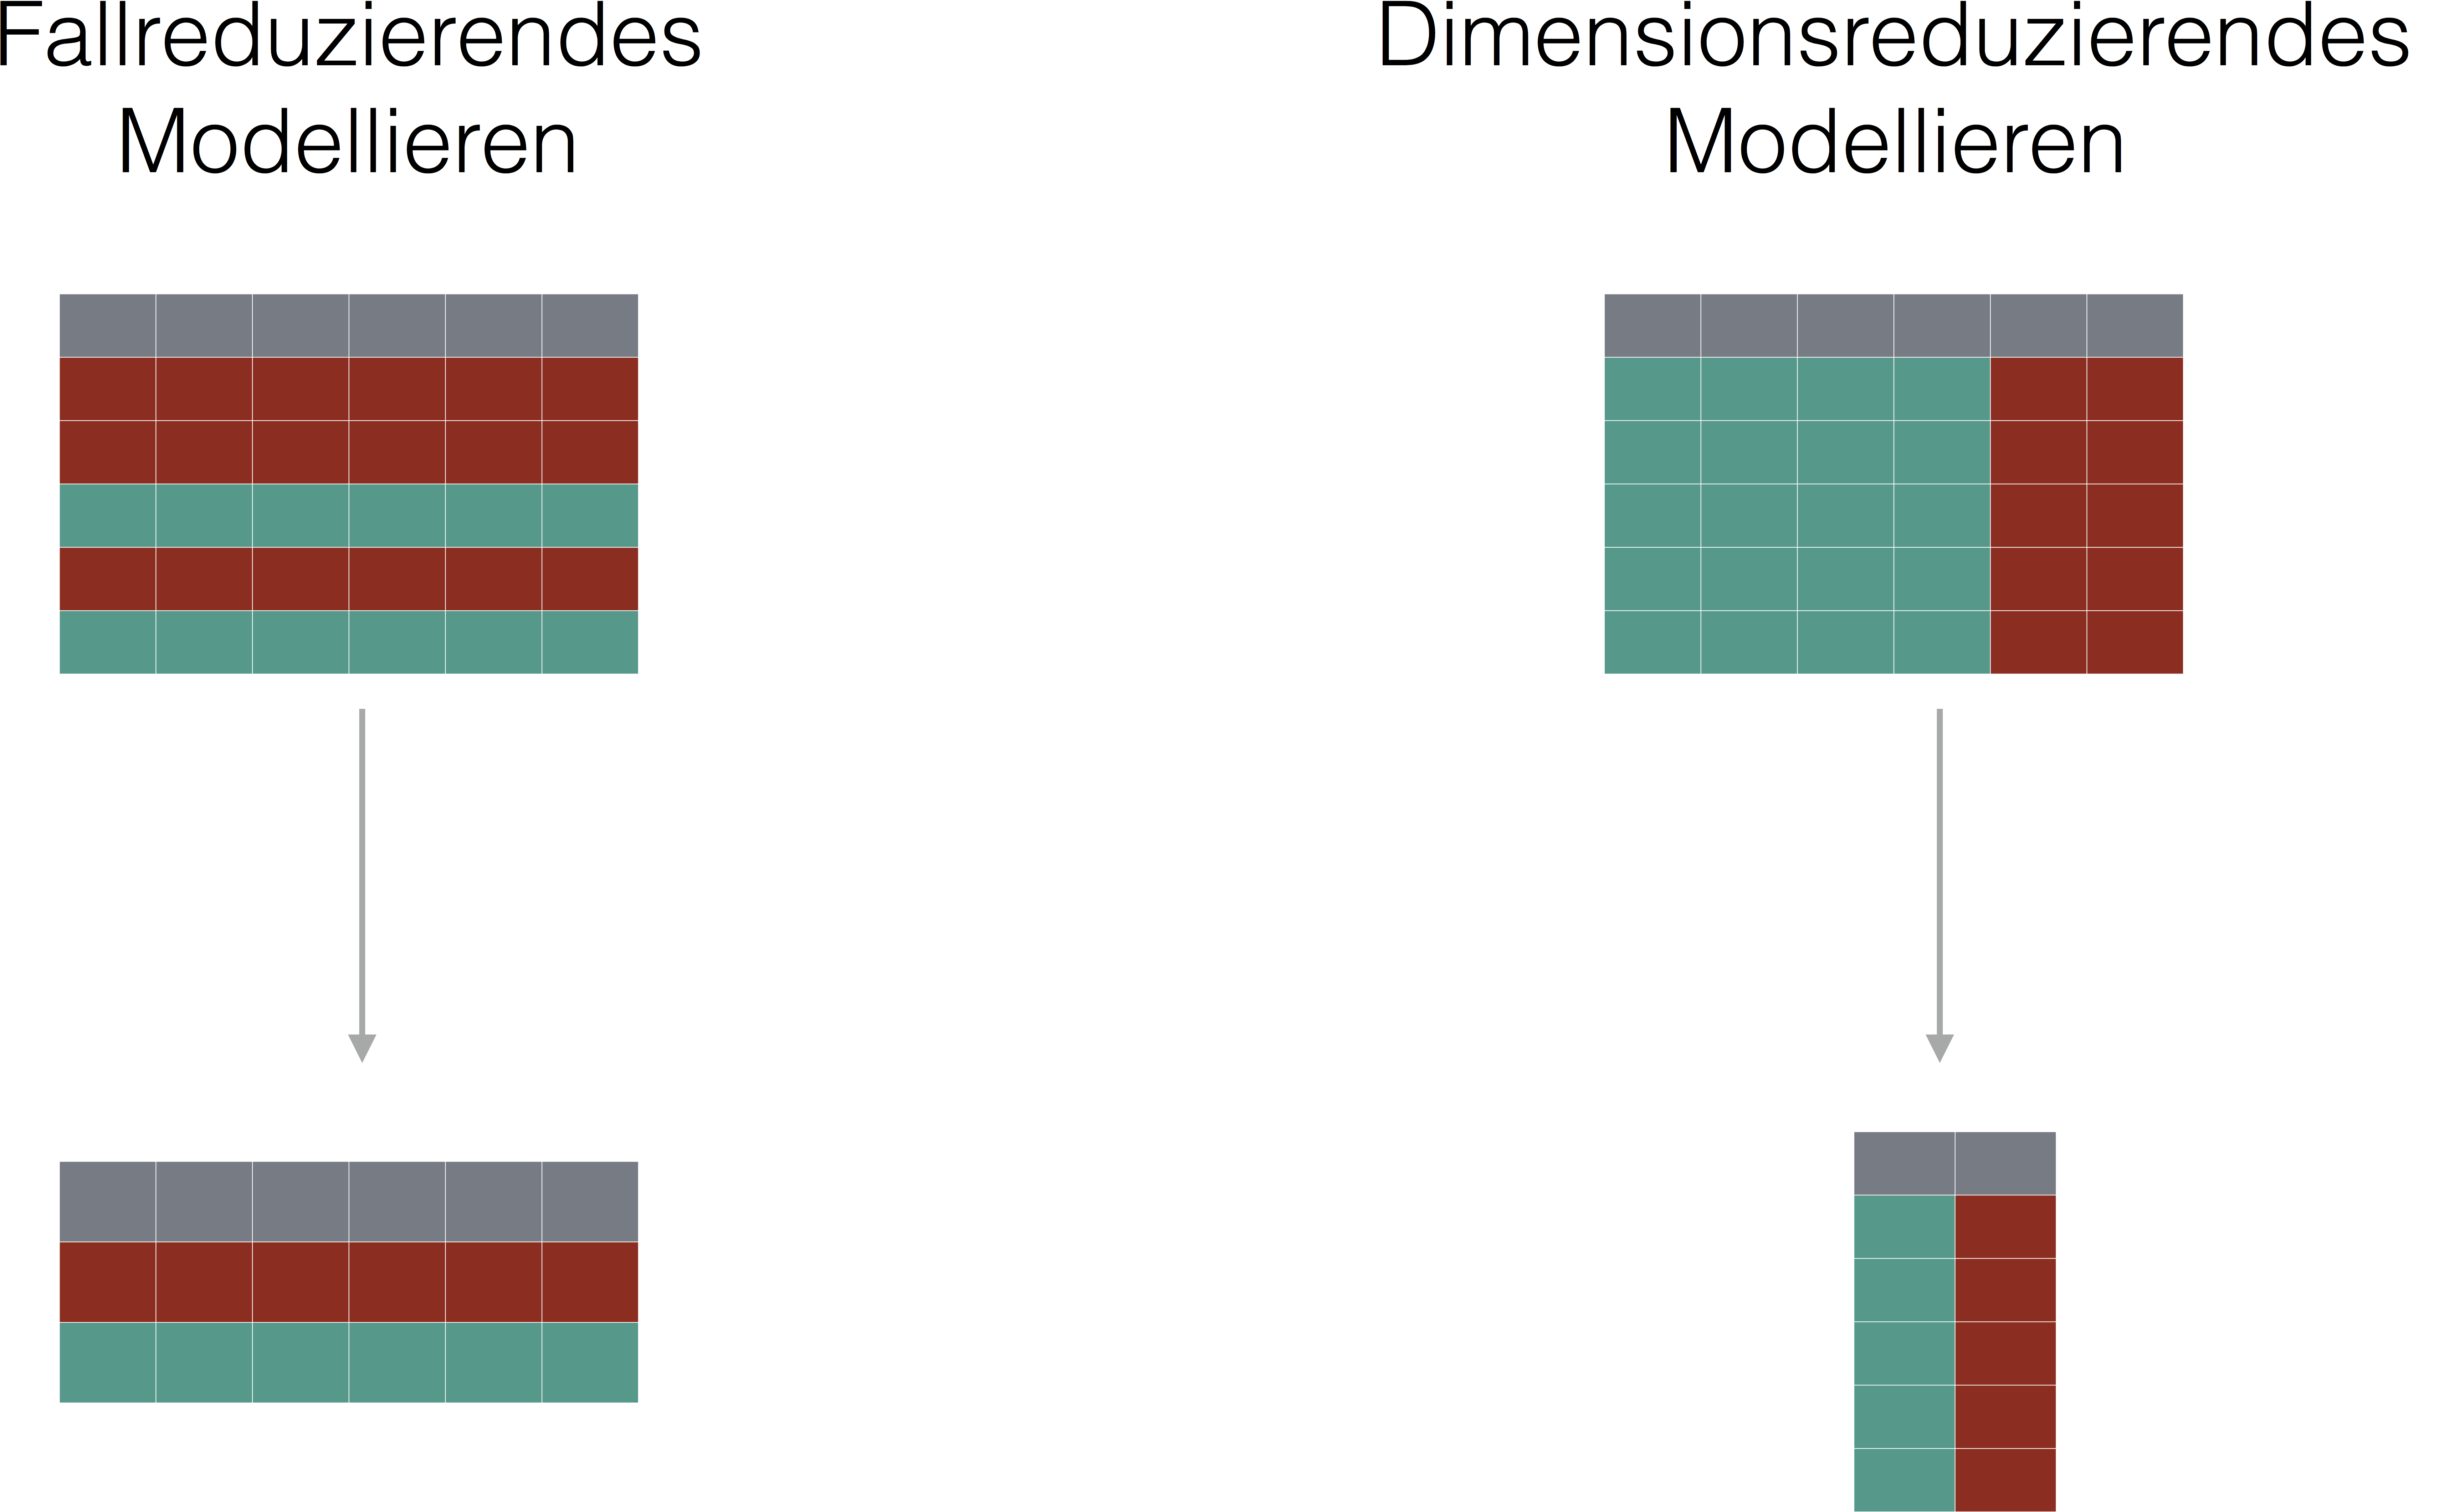
\includegraphics[width=0.8\linewidth]{../images/modellieren/ungeleitetes_Modellieren_crop} 

}

\caption{Die zwei Arten des ungeleiteten Modellierens}\label{fig:ungeleitetes-modellieren}
\end{figure}

\end{frame}

\begin{frame}{Die vier Schritte des statistischen Modellierens}

\begin{enumerate}
\def\labelenumi{\arabic{enumi}.}
\tightlist
\item
  Man wählt eines der vier Ziele des Modellierens (z.B. ein prädiktives
  Modell).
\item
  Man wählt ein Modell aus (genauer: eine Modellfamilie), z.B.
  postuliert man, dass die Körpergröße einen linearen Einfluss auf die
  Schuhgröße habe.
\item
  Man bestimmt (berechnet) die Details des Modells anhand der Daten: Wie
  groß ist die Steigung der Geraden und wo ist der Achsenabschnitt? Man
  sagt auch, dass man die \emph{Modellparameter} anhand der Daten
  schätzt (``Modellinstantiierung'' oder ``Modellanpassung'', engl.
  ``model fitting'').
\item
  Dann prüft man, wie gut das Modell zu den Daten passt (Modellgüte,
  engl. ``model fit''); wie gut lässt sich die Schuhgröße anhand der
  Körpergröße vorhersagen bzw. wie groß ist der Vorhersagefehler?
\end{enumerate}

\end{frame}

\begin{frame}{Einfache vs.~komplexe Modelle: Unter- vs.~Überanpassung}

\begin{figure}

{\centering 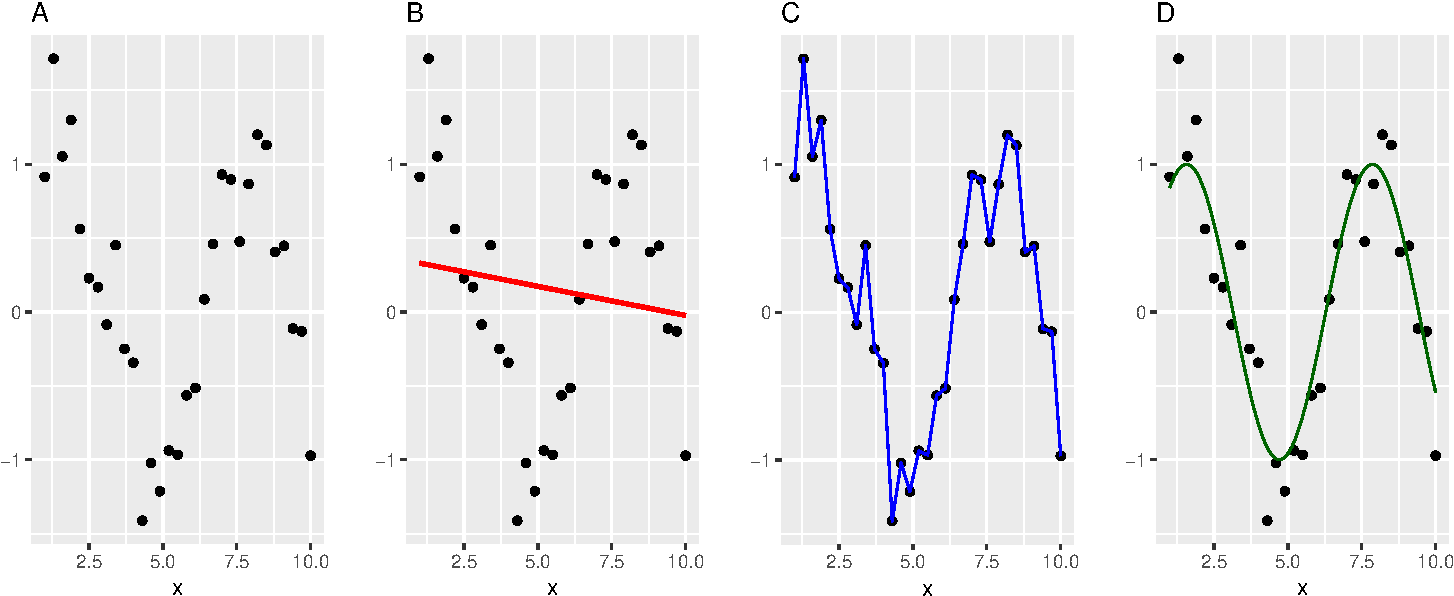
\includegraphics[width=0.9\linewidth]{PraDa_Folien_nm_2_files/figure-beamer/overfitting-4-plots-1} 

}

\caption{Welches Modell (Teil B-D; rot, grün, blau) passt am besten zu den Daten (Teil A) ?}\label{fig:overfitting-4-plots}
\end{figure}

\end{frame}

\begin{frame}{Vorhersagegüte der Trainings-Stichprobe vs.~der
Test-Stichprobe}

Beschreibt ein Modell (wie das blaue Modell hier) eine Stichprobe sehr
gut, heißt das noch \emph{nicht}, dass es auch zukünftige (und
vergleichbare) Stichproben gut beschreiben wird. Die Güte
(Vorhersagegenauigkeit) eines Modells sollte sich daher stets auf eine
neue Stichprobe beziehen (Test-Stichprobe), die nicht in der Stichprobe
beim Anpassen des Modells (Trainings-Stichprobe) enthalten war.

\end{frame}

\begin{frame}{Overfitting}

\begin{figure}

{\centering 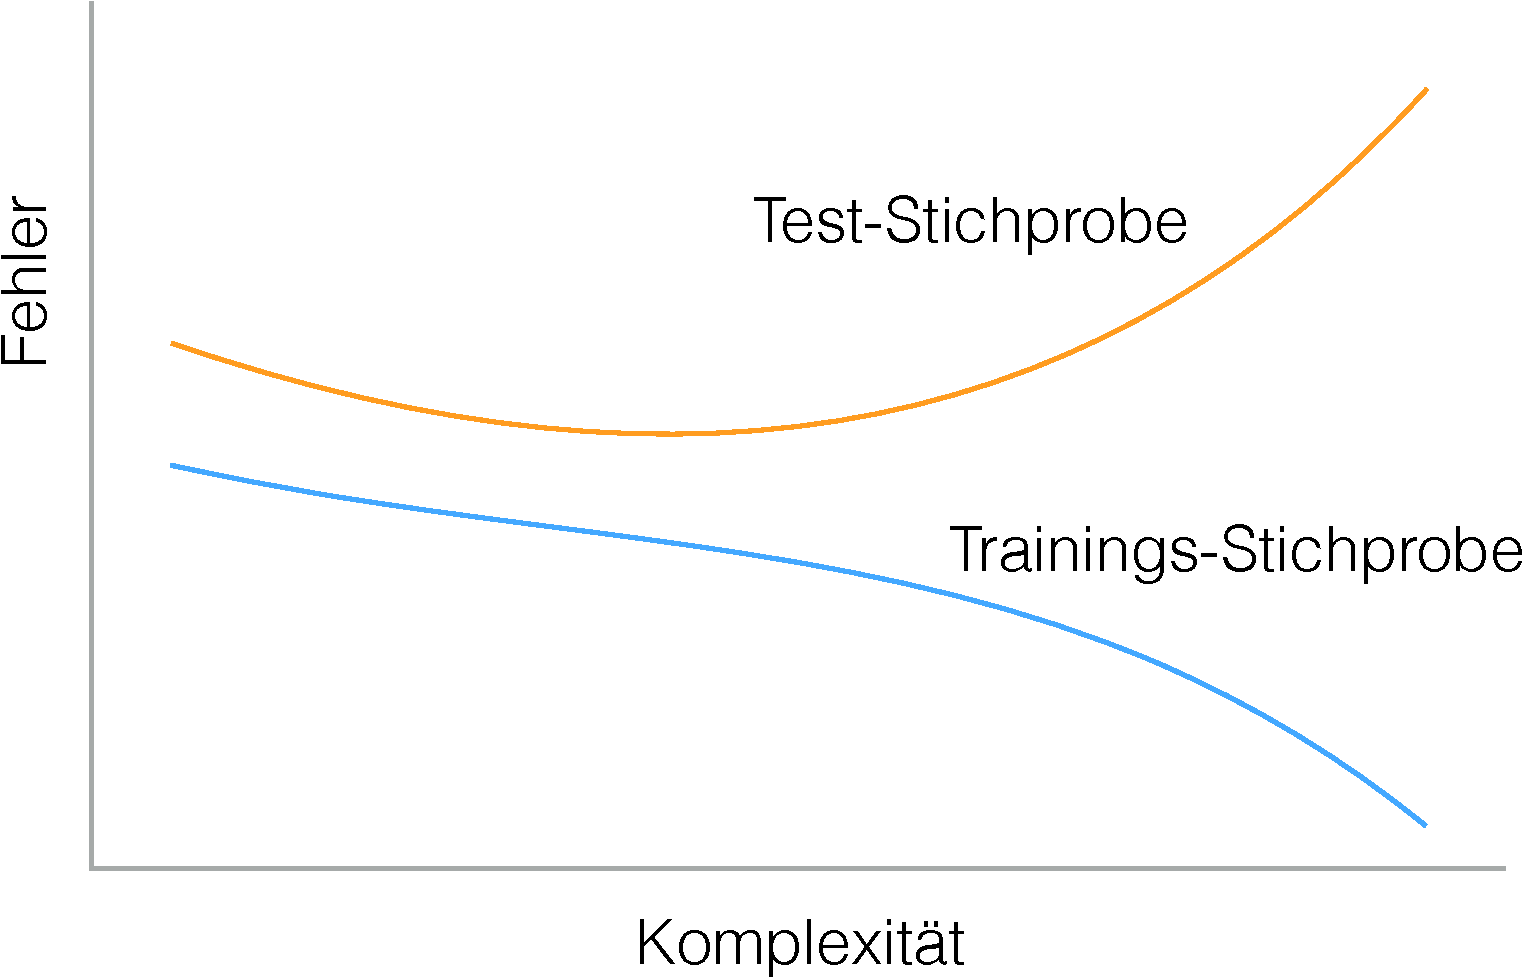
\includegraphics[width=0.5\linewidth]{../images/modellieren/overfitting} 

}

\caption{'Mittlere' Komplexität hat die beste Vorhersagegenauigkeit (am wenigsten Fehler) in der Test-Stichprobe}\label{fig:overfitting-schema}
\end{figure}

\end{frame}

\begin{frame}{Bias-Varianz-Abwägung}

\begin{quote}
Einfache Modelle: Viel Bias, wenig Varianz. Komplexe Modelle: Wenig
Bias, viel Varianz.
\end{quote}

\begin{figure}

{\centering 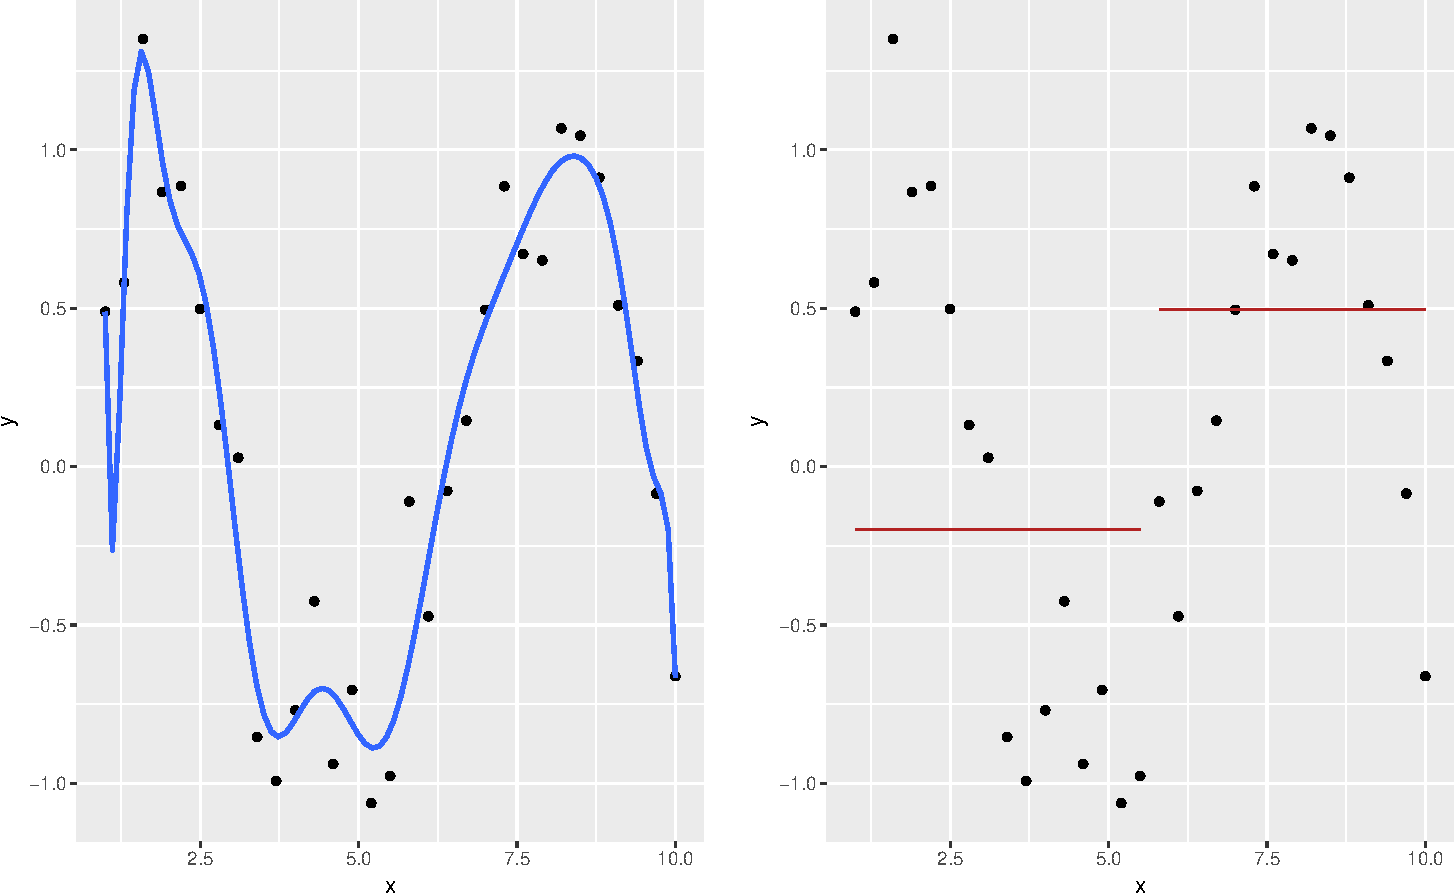
\includegraphics[width=0.5\linewidth]{PraDa_Folien_nm_2_files/figure-beamer/plot-bias-variance-1} 

}

\caption{Der Spagat zwischen Verzerrung und Varianz}\label{fig:plot-bias-variance}
\end{figure}

\end{frame}

\section{Der p-Wert}\label{p-wert}

\begin{frame}{Lernziele}

\begin{itemize}
\tightlist
\item
  Den p-Wert erläutern können.
\item
  Den p-Wert kritisieren können.
\item
  Alternativen zum p-Wert kennen.
\item
  Inferenzstatistische Verfahren für häufige Fragestellungen kennen.
\end{itemize}

\end{frame}

\begin{frame}{Sir Ronald Fisher, Erfinder des Nullhypothesen Testens}

\begin{figure}

{\centering 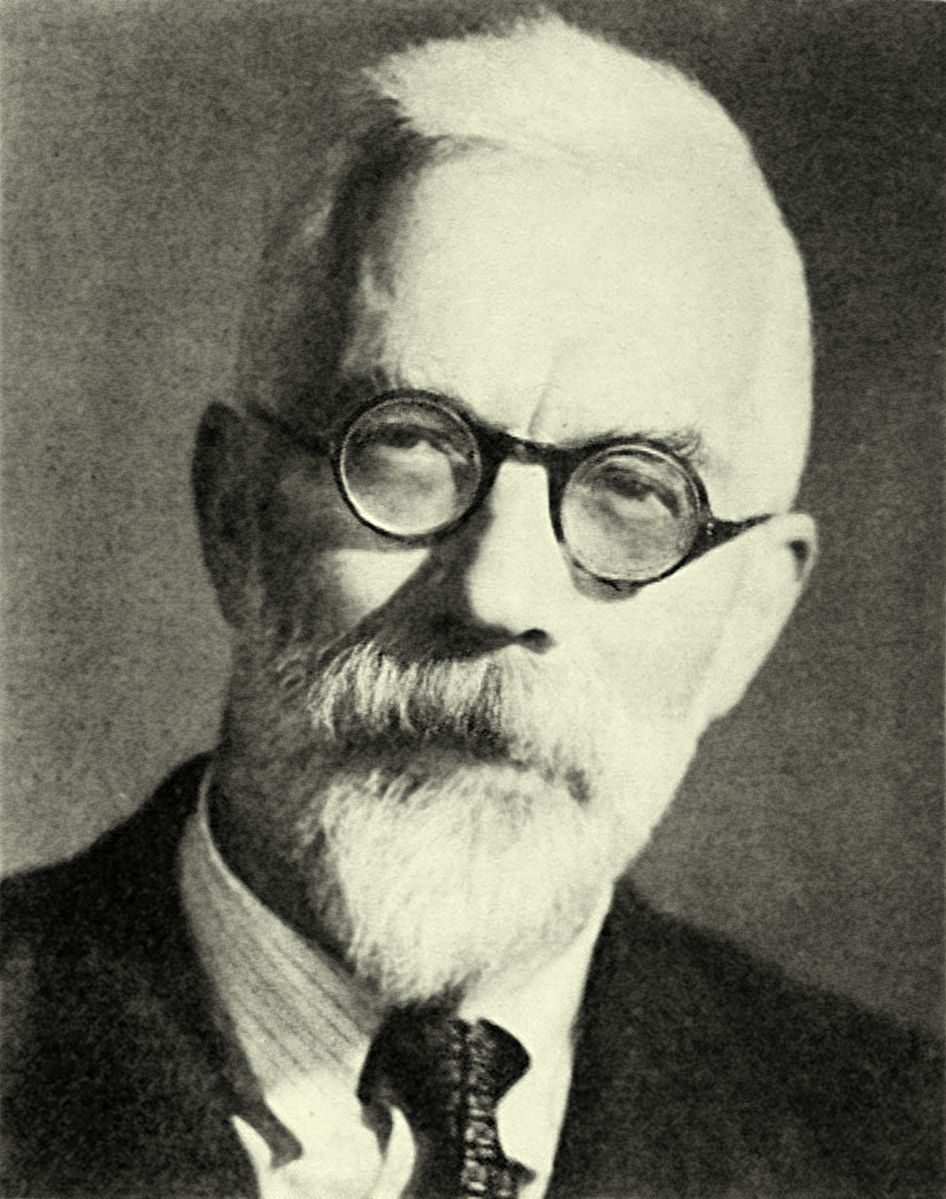
\includegraphics[width=0.2\linewidth]{../images/inferenz/Ronald_Fisher} 

}

\caption{Der größte Statistiker des 20. Jahrhunderts (p < .05)}\label{fig:sir-fisher}
\end{figure}

\end{frame}

\begin{frame}{Der p-Wert ist die heilige Kuh der Forscher}

\begin{figure}

{\centering 
\includegraphics[width=0.35\linewidth]{../images//inferenz/p_value_who_said} 

}

\caption{Der p-Wert wird oft als wichtig erachtet}\label{fig:who-said}
\end{figure}

\begin{quote}
Der p-Wert sagt, wie gut die Daten zur Nullhypothese passen.
\end{quote}

\end{frame}

\begin{frame}{Von Männern und Päpsten}

\[ P(M|P) \ne P(P|M) \]

\begin{figure}

{\centering 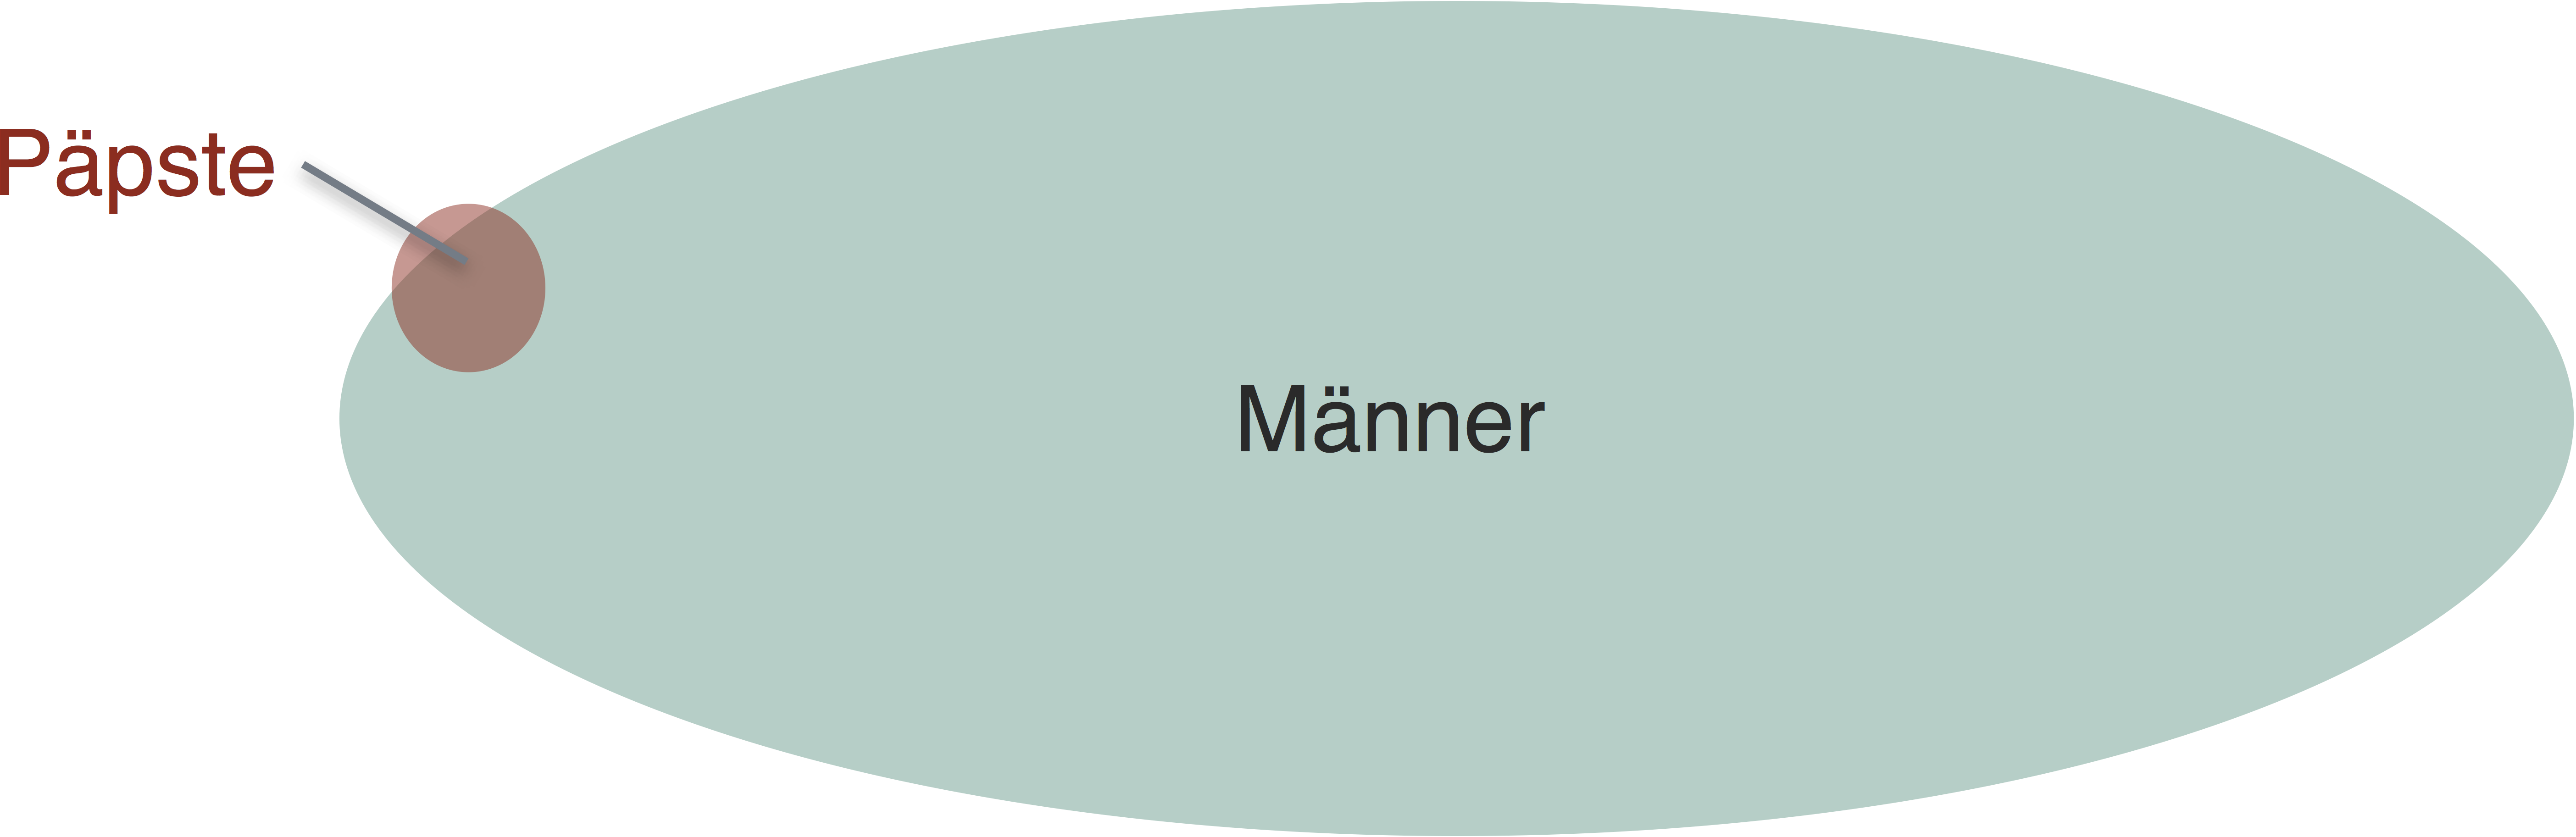
\includegraphics[width=0.8\linewidth]{../images/inferenz/maenner_papst-crop} 

}

\caption{Mann und Papst zu sein, ist nicht das gleiche.}\label{fig:moslems-terroristen}
\end{figure}

\end{frame}

\begin{frame}{Der p-Wert ist eine Funktion der Stichprobengröße}

\begin{figure}

{\centering 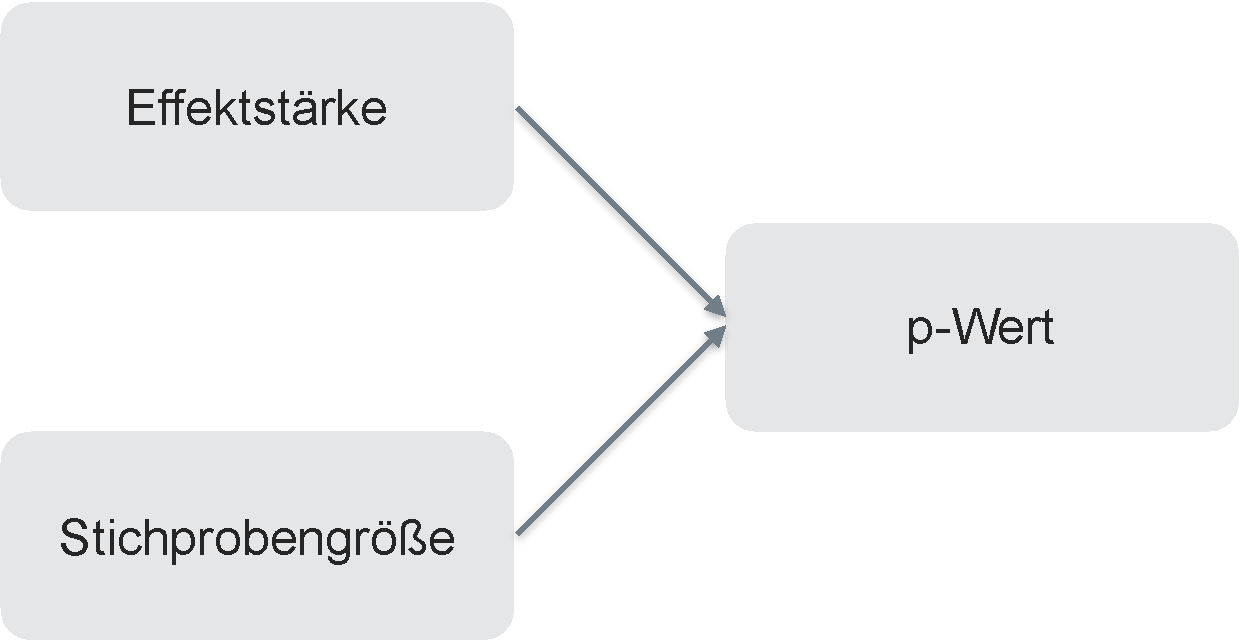
\includegraphics[width=0.8\linewidth]{../images/inferenz/einfluss_pwert-crop} 

}

\caption{Zwei Haupteinflüsse auf den p-Wert}\label{fig:einfluss-pwert}
\end{figure}

\end{frame}

\begin{frame}{Zur Philosophie des p-Werts: Frequentismus}

\begin{figure}

{\centering 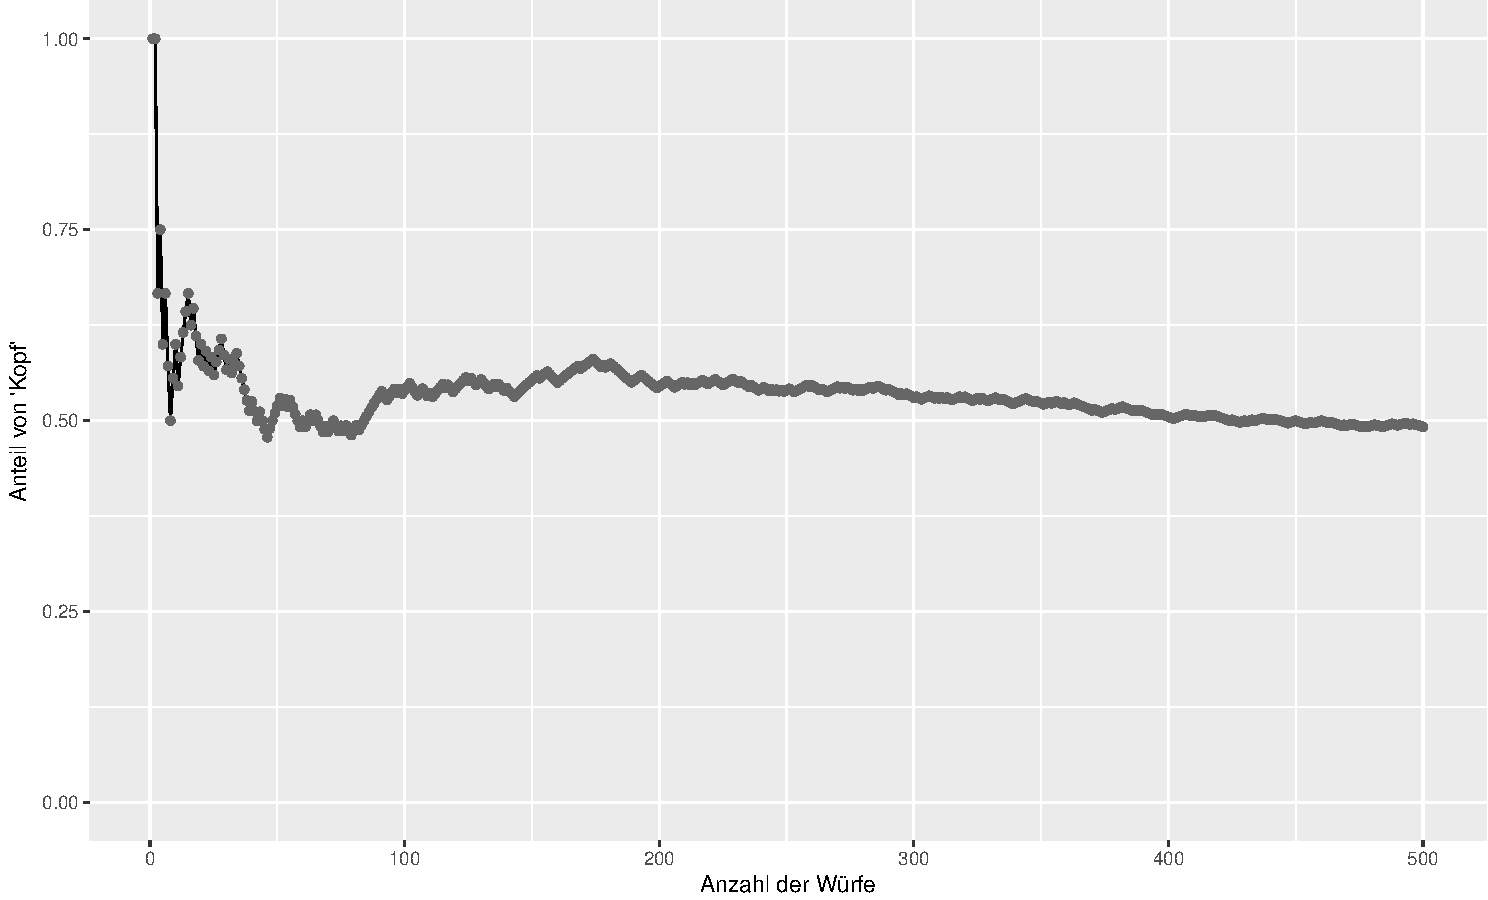
\includegraphics[width=0.8\linewidth]{PraDa_Folien_nm_2_files/figure-beamer/muenzwurf-1} 

}

\caption{Anteil von 'Kopf' bei wiederholtem Münzwurf}\label{fig:muenzwurf}
\end{figure}

\end{frame}

\begin{frame}{Alternativen zum p-Wert - Konfidenzintervalle}

\begin{quote}
Das 95\%-Konfidenzintervall ist der Bereich, in dem der Parameter in
95\% der Fälle fallen würde bei sehr häufiger Wiederholung des Versuchs.
\end{quote}

\href{http://rpsychologist.com/d3/CI/}{Visualisierung zum
Konfidenzintervall}

\end{frame}

\begin{frame}{Alternativen zum p-Wert - Effektstärken}

\begin{enumerate}
\def\labelenumi{\alph{enumi}.}
\setcounter{enumi}{18}
\tightlist
\item
  \href{https://sebastiansauer.github.io/Praxis_der_Datenanalyse/der-p-wert-inferenzstatistik-und-alternativen.html\#effektstarke}{Tabelle
  im Skript}
\end{enumerate}

\end{frame}

\begin{frame}{Alternativen zum p-Wert - Bayes-Statistik}

Bayes liefert \(p(D|H)\).

\begin{figure}

{\centering 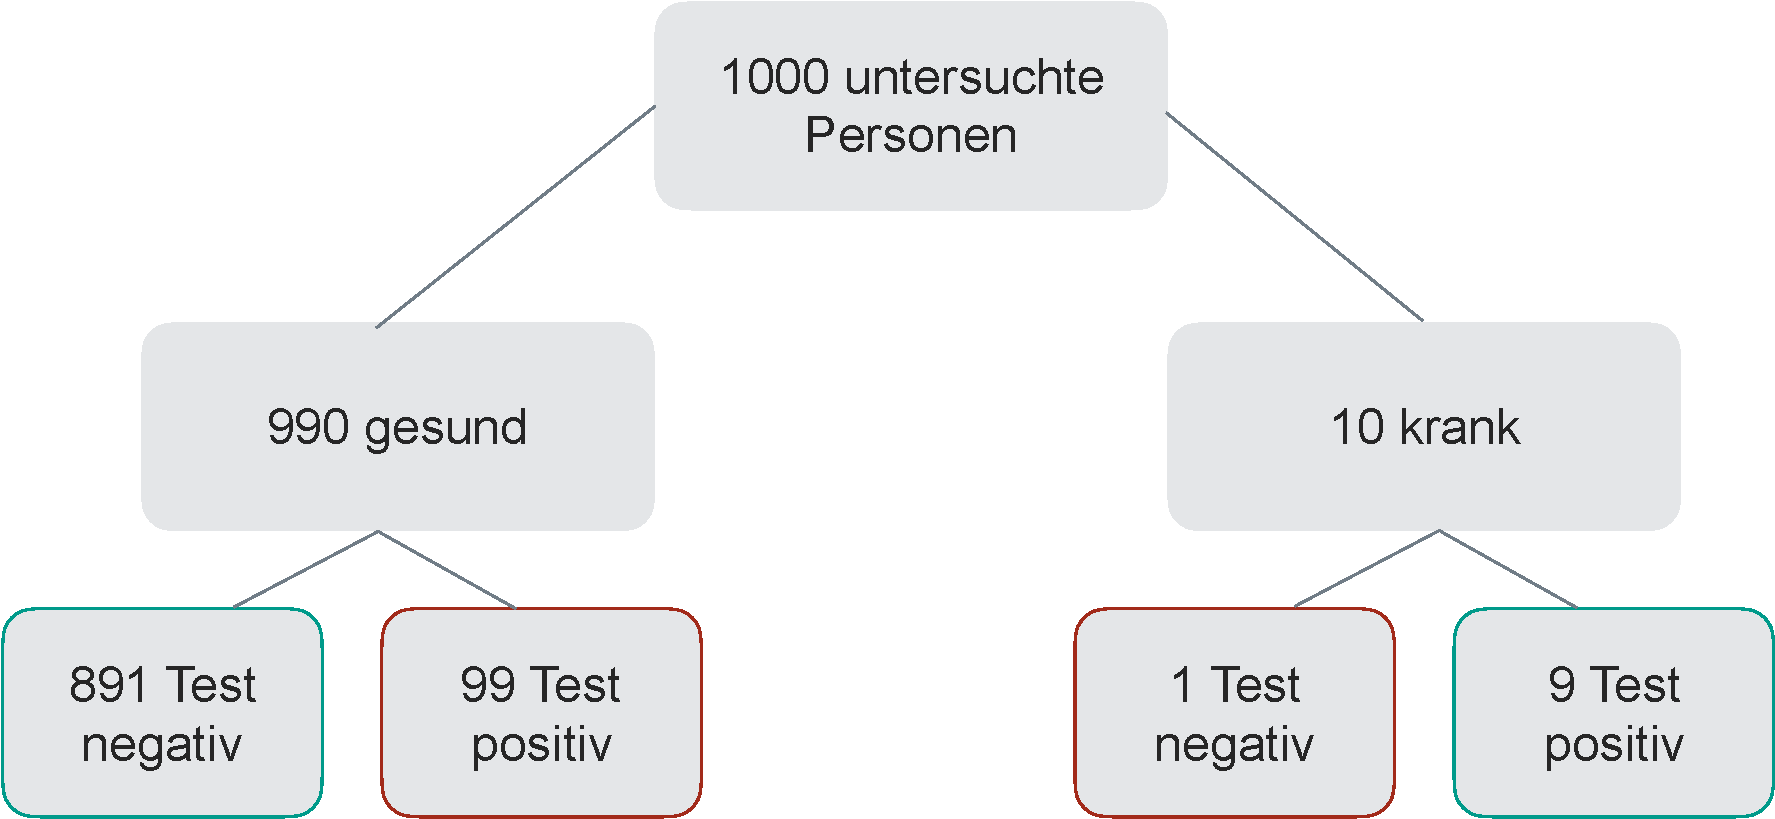
\includegraphics[width=0.8\linewidth]{../images/inferenz/bayes-crop} 

}

\caption{Die zwei Stufen der Bayes-Statistik in einem einfachen Beispieli}\label{fig:bayes}
\end{figure}

\end{frame}

\section{Lineare Regression}\label{lineare-regression}

\begin{frame}{Lernziele}

\begin{itemize}
\tightlist
\item
  Wissen, was man unter Regression versteht.
\item
  Die Annahmen der Regression überprüfen können.
\item
  Regression mit kategorialen Prädiktoren durchführen können.
\item
  Die Modellgüte bei der Regression bestimmen können.
\item
  Interaktionen erkennen und ihre Stärke einschätzen können.
\end{itemize}

\end{frame}

\begin{frame}[fragile]{Beispiel für eine lineare Regression}

\begin{verbatim}
score = achsenabschnitt + steigung*study_time
\end{verbatim}

\begin{figure}

{\centering 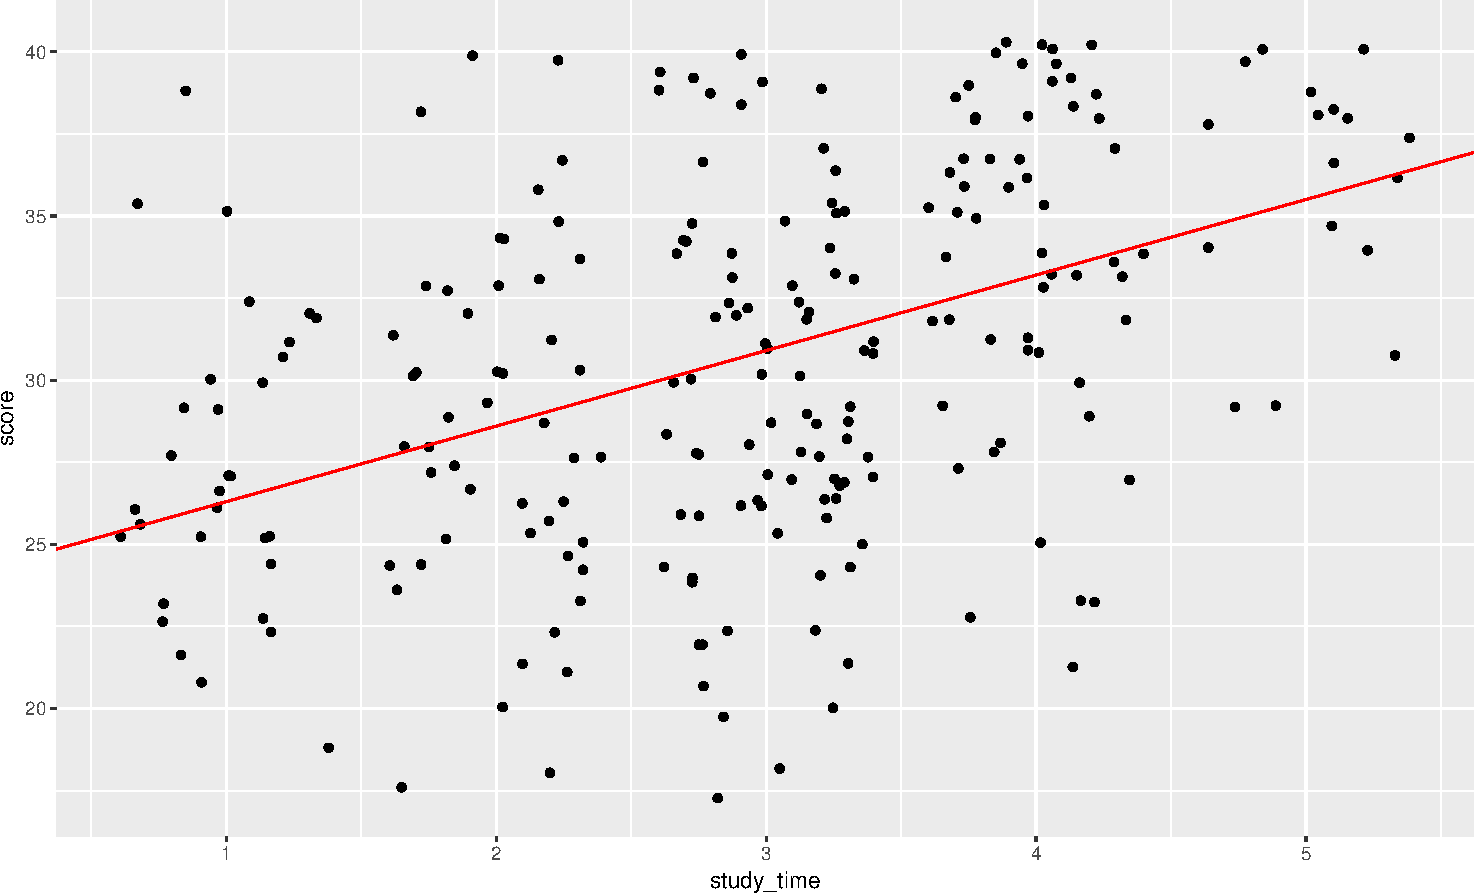
\includegraphics[width=0.5\linewidth]{PraDa_Folien_nm_2_files/figure-beamer/bsp-regression-1} 

}

\caption{Beispiel für eine Regression}\label{fig:bsp-regression}
\end{figure}

\end{frame}

\begin{frame}[fragile]{Die Formel einer einfachen Regression}

\begin{verbatim}
score = achsenabschnitt + steigung*study_time
\end{verbatim}

\end{frame}

\begin{frame}{Vorhersagegüte - Veranschaulichung}

\begin{figure}

{\centering 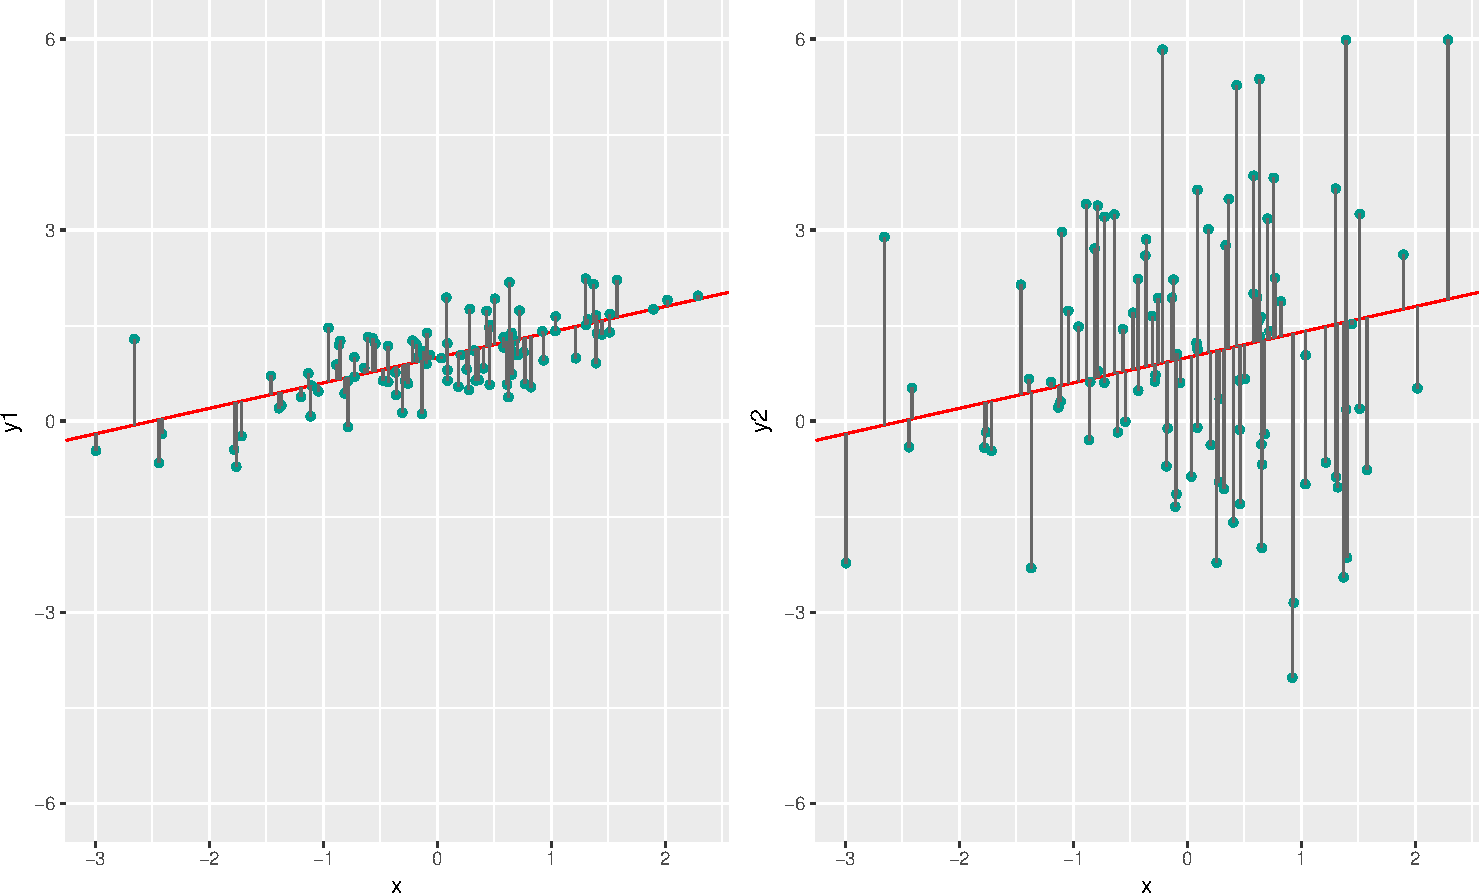
\includegraphics[width=0.8\linewidth]{PraDa_Folien_nm_2_files/figure-beamer/resids-plot-1} 

}

\caption{Geringer (links) vs. hoher (rechts) Vorhersagefehler}\label{fig:resids-plot}
\end{figure}

\end{frame}

\begin{frame}{Vorhersagegüte - MSE und \(R^2\)}

\[ MSE = \frac{1}{n} \sum{(pred - obs)^2} \]

\[ R^2 = 1 - \left( \frac{SS_T - SS_M}{SS_T} \right)\]

\end{frame}

\begin{frame}{Überprüfung der Annahmen der linearen Regression}

\begin{itemize}
\tightlist
\item
  Linearität des Zusammenhangs
\item
  Normalverteilung der Residuen
\item
  Konstante Varianz
\item
  Extreme Ausreißer
\item
  Unabhängigkeit der Beobachtungen
\end{itemize}

\end{frame}

\begin{frame}{Unterscheiden sich Interessierten von Nicht-I. im
Klausurerfolg?}

\begin{longtable}[]{@{}lr@{}}
\toprule
interessiert & score\tabularnewline
\midrule
\endhead
FALSE & 29.90909\tabularnewline
TRUE & 31.53684\tabularnewline
NA & 33.08824\tabularnewline
\bottomrule
\end{longtable}

\end{frame}

\begin{frame}[fragile]{Kategoriale Prädiktoren}

\begin{Shaded}
\begin{Highlighting}[]
<<<<<<< Updated upstream
\NormalTok{stats_test }\OperatorTok\StringTok{ }\NormalTok{na.omit }\OperatorTok\StringTok{ }\KeywordTok{ggplot}\NormalTok{() }\OperatorTok{+}\StringTok{ }\KeywordTok{aes}\NormalTok{(}\DataTypeTok{x =}\NormalTok{ interessiert, }\DataTypeTok{y =}\NormalTok{ score) }\OperatorTok{+}\StringTok{ }\KeywordTok{geom_jitter}\NormalTok{(}\DataTypeTok{width =} \FloatTok{0.1}\NormalTok{) }\OperatorTok{+}\StringTok{ }
\StringTok{    }\KeywordTok{geom_point}\NormalTok{(}\DataTypeTok{data =}\NormalTok{ score_interesse, }\DataTypeTok{color =} \StringTok{"red"}\NormalTok{, }\DataTypeTok{size =} \DecValTok{5}\NormalTok{) }\OperatorTok{+}\StringTok{ }\KeywordTok{geom_line}\NormalTok{(}\DataTypeTok{data =}\NormalTok{ score_interesse, }
=======
\NormalTok{stats_test %>%}\StringTok{ }\NormalTok{na.omit %>%}\StringTok{ }\KeywordTok{ggplot}\NormalTok{() +}\StringTok{ }\KeywordTok{aes}\NormalTok{(}\DataTypeTok{x =} \NormalTok{interessiert, }\DataTypeTok{y =} \NormalTok{score) +}\StringTok{ }\KeywordTok{geom_jitter}\NormalTok{(}\DataTypeTok{width =} \FloatTok{0.1}\NormalTok{) +}\StringTok{ }
\StringTok{    }\KeywordTok{geom_point}\NormalTok{(}\DataTypeTok{data =} \NormalTok{score_interesse, }\DataTypeTok{color =} \StringTok{"red"}\NormalTok{, }\DataTypeTok{size =} \DecValTok{5}\NormalTok{) +}\StringTok{ }\KeywordTok{geom_line}\NormalTok{(}\DataTypeTok{data =} \NormalTok{score_interesse, }
>>>>>>> Stashed changes
    \DataTypeTok{group =} \DecValTok{1}\NormalTok{, }\DataTypeTok{color =} \StringTok{"red"}\NormalTok{)}
\end{Highlighting}
\end{Shaded}

\begin{center}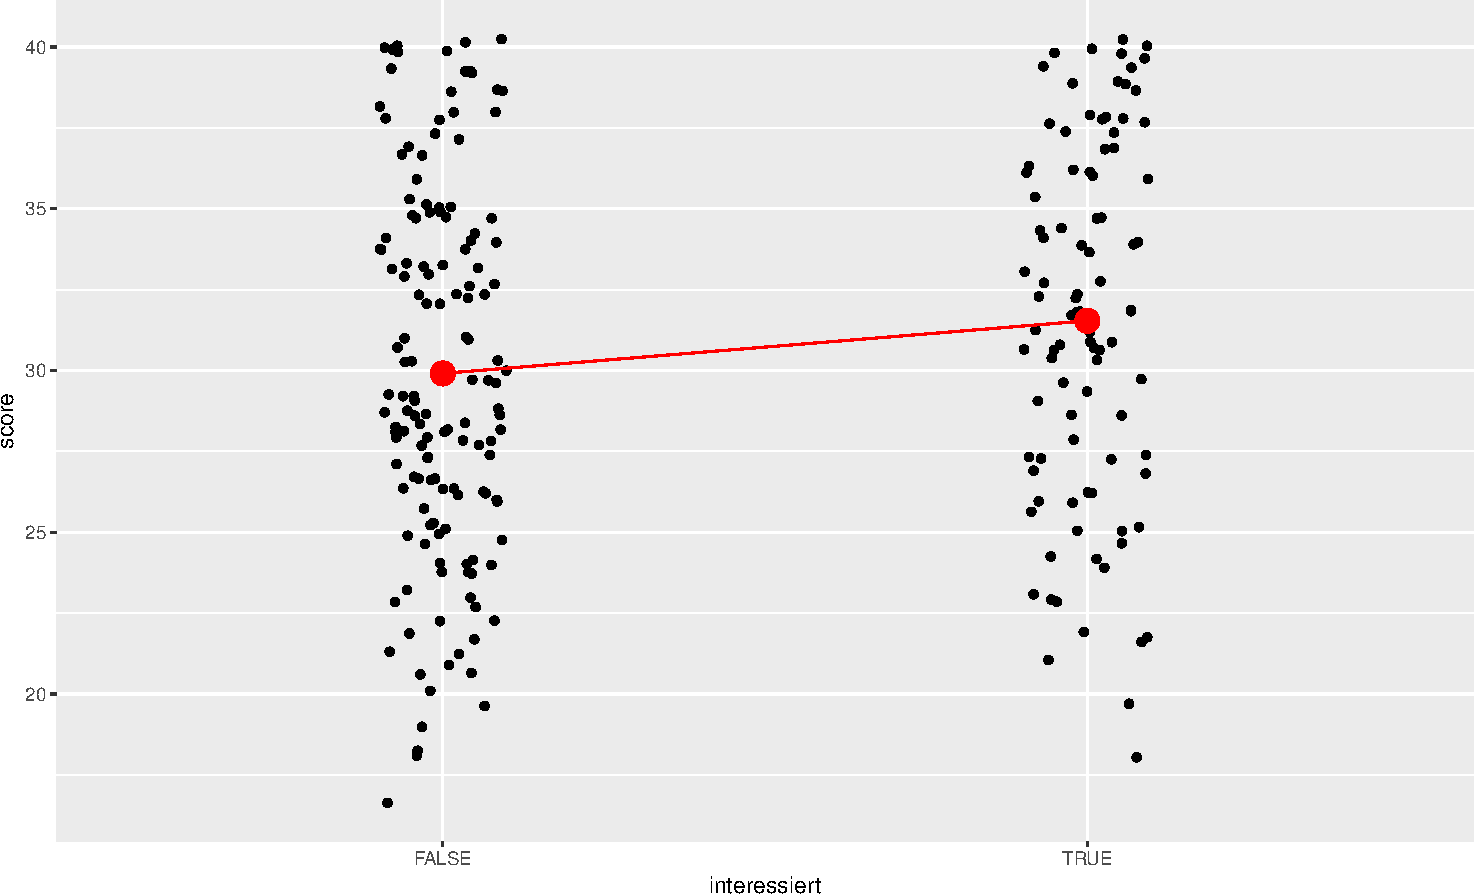
\includegraphics[width=0.8\linewidth]{PraDa_Folien_nm_2_files/figure-beamer/unnamed-chunk-13-1} \end{center}

\end{frame}

\begin{frame}{Multiple Regression}

\begin{figure}

{\centering 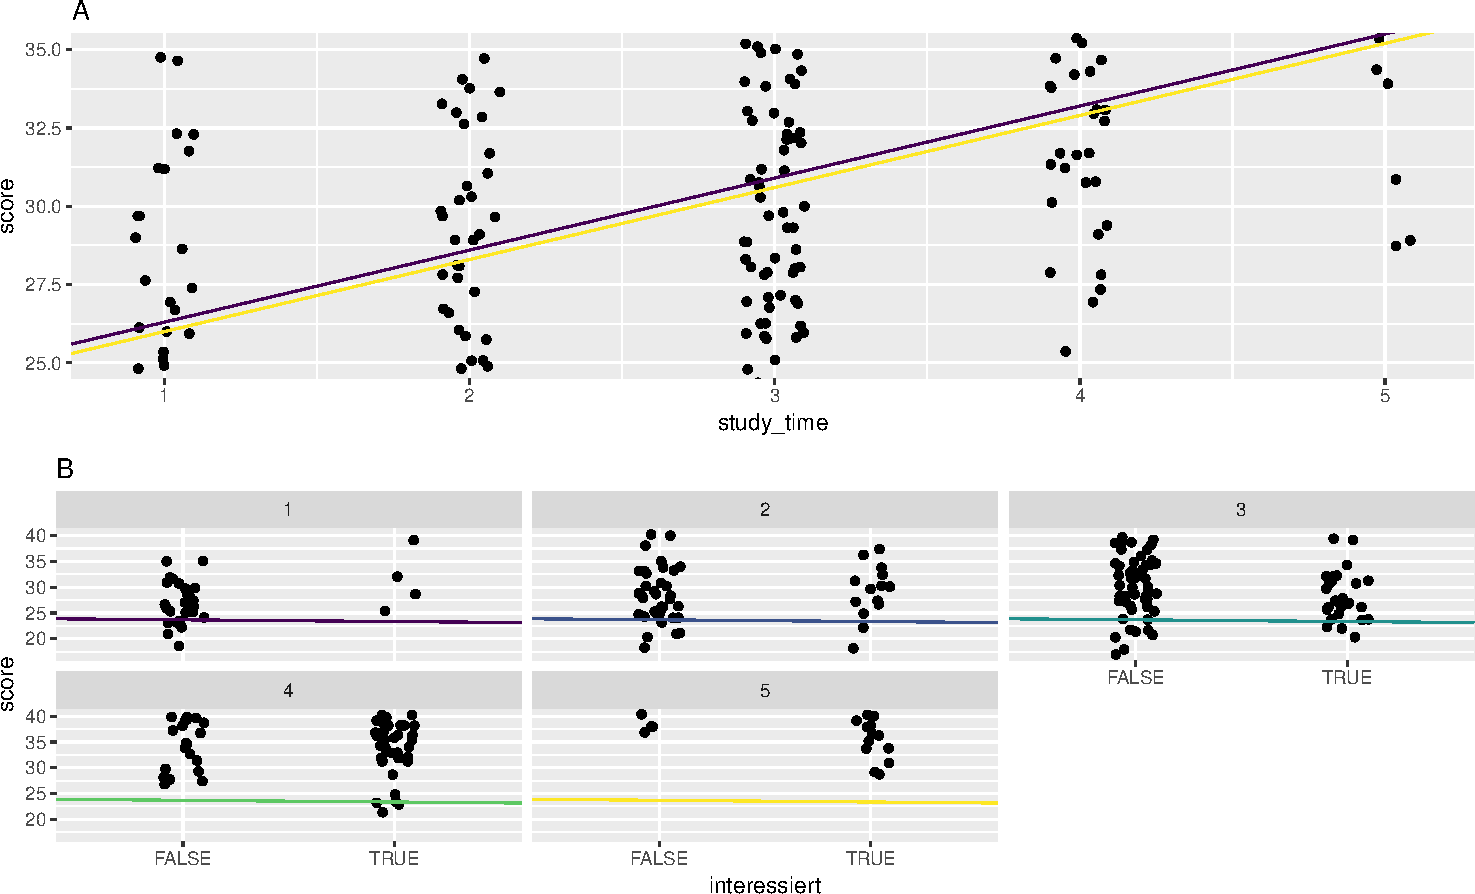
\includegraphics[width=0.8\linewidth]{PraDa_Folien_nm_2_files/figure-beamer/no-interakt-1} 

}

\caption{Eine multivariate Analyse fördert Einsichten zu Tage, die bei einfacheren Analysen verborgen bleiben}\label{fig:no-interakt}
\end{figure}

\end{frame}

\begin{frame}{Multivariate Analysen sind cool}

\begin{quote}
Die multivariate Analyse zeigt ein anderes Bild, ein genaueres Bild als
die einfachere Analyse. Ein Sachverhalt, der für den ganzen Datensatz
gilt, kann in Subgruppen anders sein.
\end{quote}

Erlaubt man der Regression, dass die Regressionsgeraden nicht parallel
sein müssen, spricht man von einer \emph{Interaktion}.

\end{frame}

\begin{frame}{Ein Beispiel für einen Interaktionseffekt}

Die Linien sind \emph{nicht} (ganz) parallel: ein kleiner
Interaktionseffekt.

\begin{figure}

{\centering 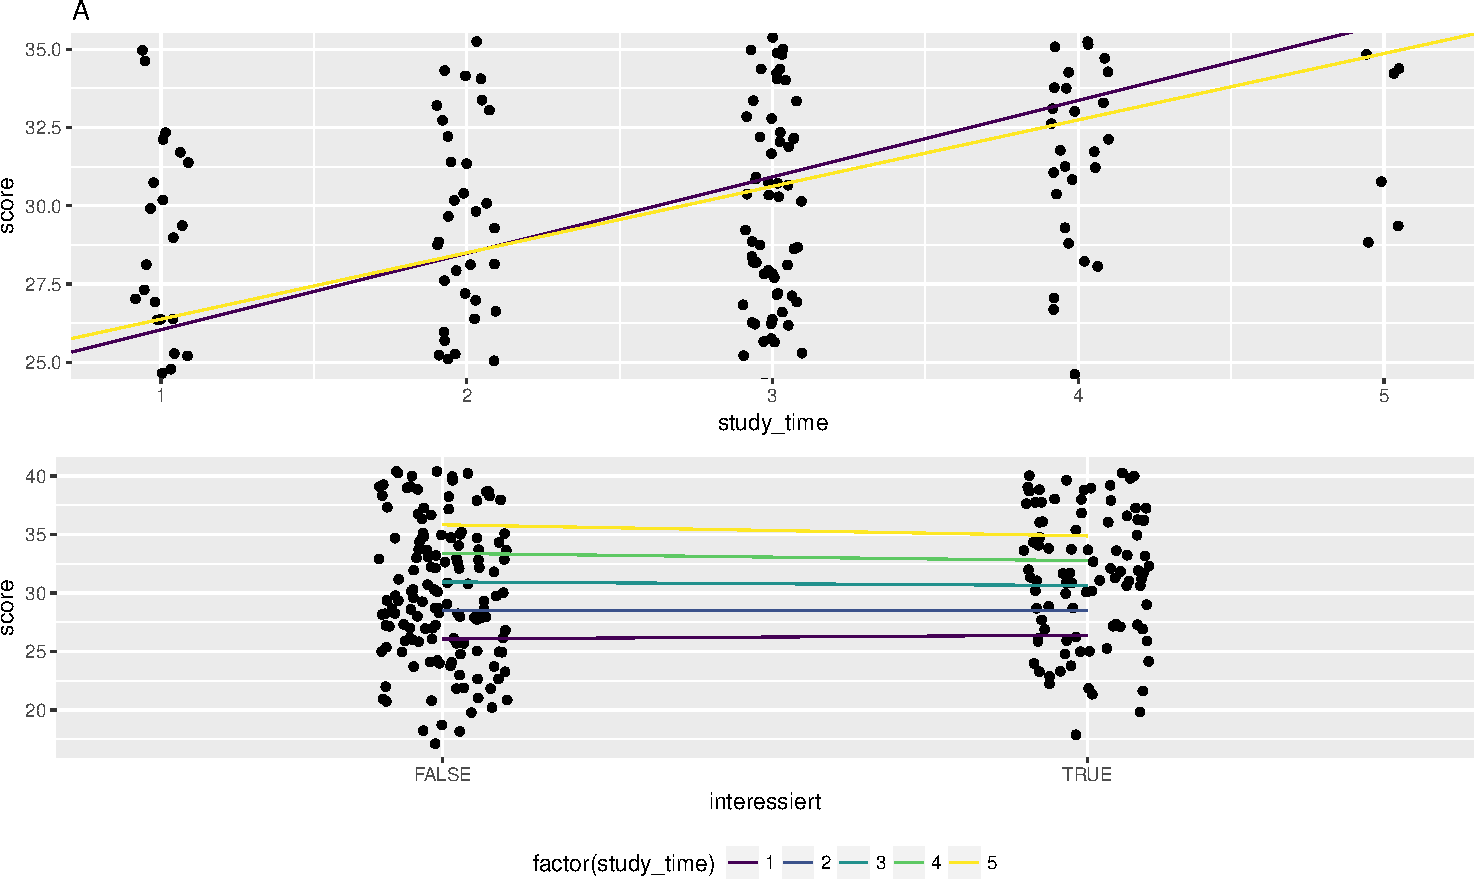
\includegraphics[width=0.8\linewidth]{PraDa_Folien_nm_2_files/figure-beamer/interakt-stats-test-1} 

}

\caption{Eine Regressionsanalyse mit Interaktionseffekten}\label{fig:interakt-stats-test}
\end{figure}

\end{frame}

\begin{frame}[fragile]{Fallstudie zu Overfitting}

\begin{Shaded}
\begin{Highlighting}[]
<<<<<<< Updated upstream
\NormalTok{caret}\OperatorTok{::}\KeywordTok{postResample}\NormalTok{(}\DataTypeTok{pred =}\NormalTok{ lm2_predict, }\DataTypeTok{obs =}\NormalTok{ test}\OperatorTok{$}\NormalTok{score)}
=======
\NormalTok{caret::}\KeywordTok{postResample}\NormalTok{(}\DataTypeTok{pred =} \NormalTok{lm2_predict, }\DataTypeTok{obs =} \NormalTok{test$score)}
>>>>>>> Stashed changes
\end{Highlighting}
\end{Shaded}

\begin{verbatim}
##     RMSE Rsquared 
## 4.433257 0.271658
\end{verbatim}

Die Modellgüte im in der Test-Stichprobe ist meist schlechter als in der
Trainings-Stichprobe. Das warnt uns vor Befunden, die naiv nur die Werte
aus der Trainings-Stichprobe berichten.

\end{frame}

\section{Klassifizierende (logistische)
Regression}\label{klassifizierende-logistische-regression}

\begin{frame}{Lernziele}

\begin{itemize}
\tightlist
\item
  Die Idee der logistischen Regression verstehen.
\item
  Die Koeffizienten der logistischen Regression interpretieren können.
\item
  Die Modellgüte einer logistischten Regression einschätzen können.
\item
  Klassifikatorische Kennzahlen kennen und beurteilen können.
\end{itemize}

\end{frame}

\begin{frame}{Problemstellung}

\begin{figure}

{\centering \includegraphics[width=0.5\linewidth]{PraDa_Folien_nm_2_files/figure-beamer/fig-logist-regr1-1} 

}

\caption{Streudiagramm von Risikobereitschaft und Aktienkauf}\label{fig:fig-logist-regr1}
\end{figure}

\end{frame}

\begin{frame}[fragile]{R-Befehl}

Die Funktion \texttt{glm} führt die logistische Regression durch.

\begin{Shaded}
\begin{Highlighting}[]
<<<<<<< Updated upstream
\NormalTok{glm1 <-}\StringTok{ }\KeywordTok{glm}\NormalTok{(Aktienkauf }\OperatorTok{~}\StringTok{ }\NormalTok{Risikobereitschaft, }\DataTypeTok{family =} \KeywordTok{binomial}\NormalTok{(}\StringTok{"logit"}\NormalTok{), }\DataTypeTok{data =}\NormalTok{ Aktien)}
=======
\NormalTok{glm1 <-}\StringTok{ }\KeywordTok{glm}\NormalTok{(Aktienkauf ~}\StringTok{ }\NormalTok{Risikobereitschaft, }\DataTypeTok{family =} \KeywordTok{binomial}\NormalTok{(}\StringTok{"logit"}\NormalTok{), }\DataTypeTok{data =} \NormalTok{Aktien)}
>>>>>>> Stashed changes
\end{Highlighting}
\end{Shaded}

\end{frame}

\begin{frame}{Visualisierung der logistischen Regression}

\begin{figure}

{\centering \includegraphics[width=0.5\linewidth]{PraDa_Folien_nm_2_files/figure-beamer/fig-logist-regr2-1} 

}

\caption{Regressionsgerade für Aktien-Modell}\label{fig:fig-logist-regr2}
\end{figure}

\end{frame}

\begin{frame}{Formel der logistischen Regression}

\begin{figure}

{\centering \includegraphics[width=0.8\linewidth]{PraDa_Folien_nm_2_files/figure-beamer/logist-curve-1} 

}

\caption{Die logistische Regression beschreibt eine 's-förmige' Kurve}\label{fig:logist-curve}
\end{figure}

\end{frame}

\begin{frame}{Die logistische Regression für die Aktien-Daten}

\begin{figure}

{\centering \includegraphics[width=0.8\linewidth]{PraDa_Folien_nm_2_files/figure-beamer/aktien-plot-1} 

}

\caption{Modelldiagramm für den Aktien-Datensatz}\label{fig:aktien-plot}
\end{figure}

\end{frame}

\begin{frame}[fragile]{Interpretation der Koeffizienten}

Ist ein Logit \(\mathfrak{L}\) größer als \(0\), so ist die zugehörige
Wahrscheinlichkeit größer als 50\% (und umgekehrt.)

\emph{Logits}\index{Logit}
\(\mathfrak{L} = ln\left( \frac{p}{1-p} \right)\)

\texttt{y\ =\ intercept\ +\ 3*Risikobereitschaft}, also

\begin{Shaded}
\begin{Highlighting}[]
<<<<<<< Updated upstream
\NormalTok{(y <-}\StringTok{ }\OperatorTok{-}\FloatTok{1.469} \OperatorTok{+}\StringTok{ }\DecValTok{3} \OperatorTok{*}\StringTok{ }\FloatTok{0.257}\NormalTok{)}
=======
\NormalTok{(y <-}\StringTok{ }\NormalTok{-}\FloatTok{1.469} \NormalTok{+}\StringTok{ }\DecValTok{3} \NormalTok{*}\StringTok{ }\FloatTok{0.257}\NormalTok{)}
>>>>>>> Stashed changes
\end{Highlighting}
\end{Shaded}

\begin{verbatim}
## [1] -0.698
\end{verbatim}

Also y = -0.698 \emph{Logits} (\(\mathfrak{L}\)).

\end{frame}

\begin{frame}[fragile]{Vorhersage individueller Wahrscheinlichkeiten}

\begin{Shaded}
\begin{Highlighting}[]
\KeywordTok{predict}\NormalTok{(glm1, }\KeywordTok{data.frame}\NormalTok{(}\DataTypeTok{Risikobereitschaft =} \DecValTok{1}\NormalTok{), }\DataTypeTok{type =} \StringTok{"response"}\NormalTok{)}
\end{Highlighting}
\end{Shaded}

\begin{verbatim}
##         1 
## 0.2294028
\end{verbatim}

\end{frame}

\begin{frame}[fragile]{Kategoriale Prädiktoren}

\begin{Shaded}
\begin{Highlighting}[]
<<<<<<< Updated upstream
\KeywordTok{str}\NormalTok{(stats_test}\OperatorTok{$}\NormalTok{bestanden)}
\NormalTok{stats_test}\OperatorTok{$}\NormalTok{bestanden <-}\StringTok{ }\KeywordTok{factor}\NormalTok{(stats_test}\OperatorTok{$}\NormalTok{bestanden, }\DataTypeTok{levels =} \KeywordTok{c}\NormalTok{(}\StringTok{"nein"}\NormalTok{, }\StringTok{"ja"}\NormalTok{))}
\NormalTok{log_stats <-}\StringTok{ }\KeywordTok{glm}\NormalTok{(bestanden }\OperatorTok{~}\StringTok{ }\NormalTok{interessiert, }\DataTypeTok{family =} \KeywordTok{binomial}\NormalTok{(}\StringTok{"logit"}\NormalTok{), }\DataTypeTok{data =}\NormalTok{ stats_test)}
=======
\KeywordTok{str}\NormalTok{(stats_test$bestanden)}
\NormalTok{stats_test$bestanden <-}\StringTok{ }\KeywordTok{factor}\NormalTok{(stats_test$bestanden, }\DataTypeTok{levels =} \KeywordTok{c}\NormalTok{(}\StringTok{"nein"}\NormalTok{, }\StringTok{"ja"}\NormalTok{))}
\NormalTok{log_stats <-}\StringTok{ }\KeywordTok{glm}\NormalTok{(bestanden ~}\StringTok{ }\NormalTok{interessiert, }\DataTypeTok{family =} \KeywordTok{binomial}\NormalTok{(}\StringTok{"logit"}\NormalTok{), }\DataTypeTok{data =} \NormalTok{stats_test)}
>>>>>>> Stashed changes
\KeywordTok{summary}\NormalTok{(log_stats)}
\end{Highlighting}
\end{Shaded}

\end{frame}

\begin{frame}{Vier Arten von Ergebnisse von Klassfikationen}

\begin{longtable}[]{@{}cc@{}}
\caption{Vier Arten von Ergebnisse von Klassfikationen (continued
below)}\tabularnewline
\toprule
<<<<<<< Updated upstream
\begin{minipage}[b]{0.34\columnwidth}\centering\strut
=======
\begin{minipage}[b]{0.31\columnwidth}\centering\strut
>>>>>>> Stashed changes
Wahrheit\strut
\end{minipage} & \begin{minipage}[b]{0.39\columnwidth}\centering\strut
Als.negativ\ldots{}..vorhergesagt\strut
\end{minipage}\tabularnewline
\midrule
\endfirsthead
\toprule
<<<<<<< Updated upstream
\begin{minipage}[b]{0.34\columnwidth}\centering\strut
=======
\begin{minipage}[b]{0.31\columnwidth}\centering\strut
>>>>>>> Stashed changes
Wahrheit\strut
\end{minipage} & \begin{minipage}[b]{0.39\columnwidth}\centering\strut
Als.negativ\ldots{}..vorhergesagt\strut
\end{minipage}\tabularnewline
\midrule
\endhead
<<<<<<< Updated upstream
\begin{minipage}[t]{0.34\columnwidth}\centering\strut
=======
\begin{minipage}[t]{0.31\columnwidth}\centering\strut
>>>>>>> Stashed changes
In Wahrheit negativ (-)\strut
\end{minipage} & \begin{minipage}[t]{0.39\columnwidth}\centering\strut
Richtig negativ (RN)\strut
\end{minipage}\tabularnewline
<<<<<<< Updated upstream
\begin{minipage}[t]{0.34\columnwidth}\centering\strut
=======
\begin{minipage}[t]{0.31\columnwidth}\centering\strut
>>>>>>> Stashed changes
In Wahrheit positiv (+)\strut
\end{minipage} & \begin{minipage}[t]{0.39\columnwidth}\centering\strut
Falsch negativ (FN)\strut
\end{minipage}\tabularnewline
<<<<<<< Updated upstream
\begin{minipage}[t]{0.34\columnwidth}\centering\strut
=======
\begin{minipage}[t]{0.31\columnwidth}\centering\strut
>>>>>>> Stashed changes
Summe\strut
\end{minipage} & \begin{minipage}[t]{0.39\columnwidth}\centering\strut
N*\strut
\end{minipage}\tabularnewline
\bottomrule
\end{longtable}

\begin{longtable}[]{@{}cc@{}}
\toprule
\begin{minipage}[b]{0.41\columnwidth}\centering\strut
Als.positiv\ldots{}..vorhergesagt\strut
\end{minipage} & \begin{minipage}[b]{0.09\columnwidth}\centering\strut
Summe\strut
\end{minipage}\tabularnewline
\midrule
\endhead
\begin{minipage}[t]{0.41\columnwidth}\centering\strut
Falsch positiv (FP)\strut
\end{minipage} & \begin{minipage}[t]{0.09\columnwidth}\centering\strut
N\strut
\end{minipage}\tabularnewline
\begin{minipage}[t]{0.41\columnwidth}\centering\strut
Richtig positiv (RN)\strut
\end{minipage} & \begin{minipage}[t]{0.09\columnwidth}\centering\strut
P\strut
\end{minipage}\tabularnewline
\begin{minipage}[t]{0.41\columnwidth}\centering\strut
P*\strut
\end{minipage} & \begin{minipage}[t]{0.09\columnwidth}\centering\strut
N+P\strut
\end{minipage}\tabularnewline
\bottomrule
\end{longtable}

\end{frame}

\begin{frame}[fragile]{Konfusionsmatrix}

\begin{verbatim}
##     obs
## pred   0   1
##    0 509 163
##    1   8  20
## attr(,"class")
## [1] "confusion.matrix"
\end{verbatim}

\begin{verbatim}
## [1] 0.1092896
\end{verbatim}

\begin{verbatim}
## [1] 0.9845261
\end{verbatim}

\end{frame}

\begin{frame}{Vier Arten von Ergebnissen einer Klassifikation}

\begin{longtable}[]{@{}ll@{}}
\caption{Geläufige Kennwerte der Klassifikation}\tabularnewline
\toprule
Name & Definition\tabularnewline
\midrule
\endfirsthead
\toprule
Name & Definition\tabularnewline
\midrule
\endhead
Falsch-Positiv-Rate (FP-Rate) & FP/N\tabularnewline
Richtig-Positiv-Rate (RP-Rate) & RP/N\tabularnewline
Falsch-Negativ-Rate (FN-Rate) & FN/N\tabularnewline
Richtig-Negativ-Rate (RN-Rate) & RN/N\tabularnewline
Positiver Vorhersagewert & RP/P*\tabularnewline
Negativer Vorhersagewert & RN/N*\tabularnewline
Gesamtgenauigkeitsrate & (RP+RN) / (N+P)\tabularnewline
\bottomrule
\end{longtable}

\end{frame}

\begin{frame}[fragile]{ROC-Kurven}

\begin{Shaded}
\begin{Highlighting}[]
<<<<<<< Updated upstream
\NormalTok{lets_roc <-}\StringTok{ }\KeywordTok{roc}\NormalTok{(Aktien}\OperatorTok{$}\NormalTok{Aktienkauf, glm1}\OperatorTok{$}\NormalTok{fitted.values)}
=======
\NormalTok{lets_roc <-}\StringTok{ }\KeywordTok{roc}\NormalTok{(Aktien$Aktienkauf, glm1$fitted.values)}
>>>>>>> Stashed changes
\KeywordTok{plot}\NormalTok{(lets_roc)}
\end{Highlighting}
\end{Shaded}

\begin{center}\includegraphics[width=0.8\linewidth]{PraDa_Folien_nm_2_files/figure-beamer/unnamed-chunk-22-1} \end{center}

\end{frame}

\begin{frame}{Beispiele für ROC-Kurven}

\begin{figure}

{\centering \includegraphics[width=0.8\linewidth]{PraDa_Folien_nm_2_files/figure-beamer/example-rocs-1} 

}

\caption{Beispiel für eine sehr gute (A), gute (B) und schlechte (C) Klassifikation}\label{fig:example-rocs}
\end{figure}

\end{frame}

\section{Clusteranalyse}\label{clusteranalyse}

\begin{frame}{Lernziele}

\begin{itemize}
\tightlist
\item
  Das Ziel einer Clusteranalyse erläutern können.
\item
  Das Konzept der euklidischen Abstände verstehen.
\item
  Eine k-Means-Clusteranalyse berechnen und interpretieren können.
\end{itemize}

\end{frame}

\begin{frame}{Clustern Sie diesen Datensatz!}

\begin{figure}

{\centering \includegraphics[width=0.8\linewidth]{PraDa_Folien_nm_2_files/figure-beamer/cluster1-1} 

}

\caption{Ein Streudiagramm - sehen Sie Gruppen (Cluster) ?}\label{fig:cluster1}
\end{figure}

\end{frame}

\begin{frame}{Intuitive Darstellung der Clusteranalayse}

\begin{figure}

{\centering \includegraphics[width=0.8\linewidth]{PraDa_Folien_nm_2_files/figure-beamer/cluster2-1} 

}

\caption{Ein Streudiagramm - mit drei Clustern}\label{fig:cluster2}
\end{figure}

\end{frame}

\begin{frame}{Unterschiedliche Anzahlen von Clustern im Vergleich}

\begin{figure}

{\centering \includegraphics[width=0.8\linewidth]{PraDa_Folien_nm_2_files/figure-beamer/cluster3-1} 

}

\caption{Unterschiedliche Anzahlen von Clustern im Vergleich}\label{fig:cluster3}
\end{figure}

\end{frame}

\begin{frame}{Wie groß ist der ``Abstand'' zwischen Anna und Berta?}

\begin{figure}

{\centering \includegraphics[width=0.5\linewidth]{../images/cluster/distanz_crop} 

}

\caption{Distanz zwischen zwei Punkten in der Ebene}\label{fig:distanz}
\end{figure}

\end{frame}

\begin{frame}{Pythagoras strikes back}

\[c^2 = a^2 + b^2\]

In unserem Beispiel heißt das \(c^2 = 3^2+4^2 = 25\). Folglich ist
\(\sqrt{c^2}=\sqrt{25}=5\). Der Abstand oder der Unterschied zwischen
Anna und Berta beträgt also 5 - diese Art von ``Abstand'' nennt man den
\emph{euklidischen Abstand}.

\end{frame}

\begin{frame}{Pythagoras in 3D}

\begin{figure}

{\centering \includegraphics[width=0.5\linewidth]{../images/cluster/pythagoras2_crop} 

}

\caption{Pythagoras in 3D}\label{fig:pythagoras2}
\end{figure}

\end{frame}

\begin{frame}{Pythagoras in Reihe geschaltet}

\begin{figure}

{\centering \includegraphics[width=0.8\linewidth]{../images/cluster/pythagoras_crop} 

}

\caption{Pythagoras in Reihe geschaltet}\label{fig:pythagoras}
\end{figure}

\end{frame}

\begin{frame}{Wie viele Cluster sind ``richtig''?}

\begin{figure}

{\centering \includegraphics[width=0.5\linewidth]{PraDa_Folien_nm_2_files/figure-beamer/cluster4-1} 

}

\caption{Die Summe der Varianz within in Abhängigkeit von der Anzahl von Clustern. Ein Screeplot.}\label{fig:cluster4}
\end{figure}

\end{frame}

\begin{frame}{k-Means Clusteranalyse}

\begin{center}\includegraphics[width=0.8\linewidth]{PraDa_Folien_nm_2_files/figure-beamer/unnamed-chunk-24-1} \end{center}

\end{frame}

\section{Dimensionsreduktion}\label{dimensionsreduktion}

\begin{frame}{Lernziele}

\begin{itemize}
\tightlist
\item
  Den Unterschied zwischen einer Hauptkomponentenanalyse und einer
  Exploratorische Faktorenanalyse kennen
\item
  Methoden kennen, um die Anzahl von Dimensionen zu bestimmen
\item
  Methoden der Visualisierung anwenden können
\item
  Umsetzungsmethoden in R anwenden können
\item
  Ergebnisse interpretieren können.
\end{itemize}

\end{frame}

\begin{frame}{PCA vs.~EFA}

\begin{itemize}
\tightlist
\item
  Die \emph{Hauptkomponentenanalyse} (engl. principal component
  analysis, PCA)

  \begin{itemize}
  \tightlist
  \item
    reduziert Daten
  \item
    erklärt die Gesamtvarianz
  \end{itemize}
\item
  Die \emph{Exploratorische Faktorenanalyse (EFA)}

  \begin{itemize}
  \tightlist
  \item
    führt manifeste Variablen (Items) auf latente Faktoren zurück
  \item
    erklärt nicht die komplette Varianz, sondern nur die Varianz, die
    durch die vorhandenen Variablen erklärt wird
  \end{itemize}
\end{itemize}

\end{frame}

\begin{frame}{Nutzen der Dimensionsreduktion}

\begin{itemize}
\item
  \emph{Dimensionen reduzieren}
\item
  \emph{Unsicherheit verringern}
\item
  \emph{Aufwand verringern}
\end{itemize}

\end{frame}

\begin{frame}{Intuition zur Dimensionsreduktion}

\begin{figure}

{\centering \includegraphics[width=0.8\linewidth]{PraDa_Folien_nm_2_files/figure-beamer/fig-scatter3d-1} 

}

\caption{Der Pfeil ist eindimensional; reduziert also die drei Dimensionen auf eine}\label{fig:fig-scatter3d}
\end{figure}

\end{frame}

\begin{frame}{Datensatz \texttt{Werte} -- z-transformiert}

\begin{longtable}[]{@{}rrrrr@{}}
\toprule
W1 & W3 & W4 & W6 & W7\tabularnewline
\midrule
\endhead
0.5149008 & 0.5961663 & 1.6629148 & 1.3261145 & 1.2935031\tabularnewline
-1.4990528 & 1.2759455 & -0.6949935 & -1.4505072 &
-1.5356813\tabularnewline
-2.1703707 & 1.2759455 & -0.6949935 & 1.3261145 &
1.2935031\tabularnewline
1.1862187 & 1.2759455 & 1.6629148 & 0.2154658 &
-0.4040075\tabularnewline
-1.4990528 & -0.7633920 & -0.6949935 & 0.2154658 &
0.1618293\tabularnewline
\bottomrule
\end{longtable}

\end{frame}

\begin{frame}[fragile]{Korrelationsplot}

\begin{Shaded}
\begin{Highlighting}[]
<<<<<<< Updated upstream
\NormalTok{corrplot}\OperatorTok{::}\KeywordTok{corrplot}\NormalTok{(}\KeywordTok{cor}\NormalTok{(Werte.sc), }\DataTypeTok{order =} \StringTok{"hclust"}\NormalTok{)}
=======
\NormalTok{corrplot::}\KeywordTok{corrplot}\NormalTok{(}\KeywordTok{cor}\NormalTok{(Werte.sc), }\DataTypeTok{order =} \StringTok{"hclust"}\NormalTok{)}
>>>>>>> Stashed changes
\end{Highlighting}
\end{Shaded}

\begin{center}\includegraphics[width=0.5\linewidth]{PraDa_Folien_nm_2_files/figure-beamer/unnamed-chunk-27-1} \end{center}

\end{frame}

\begin{frame}[fragile]{PCA berechnen}

\begin{Shaded}
\begin{Highlighting}[]
\NormalTok{Werte.pc <-}\StringTok{ }\KeywordTok{prcomp}\NormalTok{(Werte.sc)  }\CommentTok{# Principal Components berechnen}
\KeywordTok{summary}\NormalTok{(Werte.pc)}

<<<<<<< Updated upstream
\NormalTok{Gesamtvarianz <-}\StringTok{ }\KeywordTok{sum}\NormalTok{(Werte.pc}\OperatorTok{$}\NormalTok{sdev}\OperatorTok{^}\DecValTok{2}\NormalTok{)}

\CommentTok{# Varianzanteil der ersten Hauptkomponente}
\NormalTok{Werte.pc}\OperatorTok{$}\NormalTok{sdev[}\DecValTok{1}\NormalTok{]}\OperatorTok{^}\DecValTok{2}\OperatorTok{/}\NormalTok{Gesamtvarianz}
=======
\NormalTok{Gesamtvarianz <-}\StringTok{ }\KeywordTok{sum}\NormalTok{(Werte.pc$sdev^}\DecValTok{2}\NormalTok{)}

\CommentTok{# Varianzanteil der ersten Hauptkomponente}
\NormalTok{Werte.pc$sdev[}\DecValTok{1}\NormalTok{]^}\DecValTok{2}\NormalTok{/Gesamtvarianz}
>>>>>>> Stashed changes
\end{Highlighting}
\end{Shaded}

\end{frame}

\begin{frame}[fragile]{Scree-Plot}

\begin{Shaded}
\begin{Highlighting}[]
\KeywordTok{plot}\NormalTok{(Werte.pc, }\DataTypeTok{type =} \StringTok{"l"}\NormalTok{)}
\end{Highlighting}
\end{Shaded}

\begin{figure}

{\centering \includegraphics[width=0.8\linewidth]{PraDa_Folien_nm_2_files/figure-beamer/pca-scree-1} 

}

\caption{Screeplot}\label{fig:pca-scree}
\end{figure}

\end{frame}

\begin{frame}[fragile]{Eigenwert-Kriterium}

Der \emph{Eigenwert}\index{Eigenwert} ist eine Metrik für den Anteil der
erklärten Varianz pro Hauptkomponente.

\begin{Shaded}
\begin{Highlighting}[]
\KeywordTok{eigen}\NormalTok{(}\KeywordTok{cor}\NormalTok{(Werte))}
\end{Highlighting}
\end{Shaded}

Laut dem Eigenwert-Kriterium sollen nur Faktoren mit einem
\emph{Eigenwert größer 1} extrahiert werden.

\end{frame}

\begin{frame}[fragile]{Screeplot}

\begin{Shaded}
\begin{Highlighting}[]
\KeywordTok{VSS.scree}\NormalTok{(Werte)}
\end{Highlighting}
\end{Shaded}

\begin{figure}

{\centering \includegraphics[width=0.8\linewidth]{PraDa_Folien_nm_2_files/figure-beamer/vss-scree-1} 

}

\caption{VSS-Screeplot}\label{fig:vss-scree}
\end{figure}

\end{frame}

\begin{frame}[fragile]{Biplot}

\begin{Shaded}
\begin{Highlighting}[]
\KeywordTok{biplot}\NormalTok{(Werte.pc)}
\end{Highlighting}
\end{Shaded}

\begin{center}\includegraphics[width=0.5\linewidth]{PraDa_Folien_nm_2_files/figure-beamer/unnamed-chunk-28-1} \end{center}

\end{frame}

\begin{frame}[fragile]{Ladungen der Items auf die Hauptkomponenten}

\begin{Shaded}
\begin{Highlighting}[]
\NormalTok{Werte.pca <-}\StringTok{ }\KeywordTok{principal}\NormalTok{(Werte, }\DataTypeTok{nfactors =} \DecValTok{5}\NormalTok{, }\DataTypeTok{rotate =} \StringTok{"none"}\NormalTok{)}
\end{Highlighting}
\end{Shaded}

\end{frame}

\begin{frame}[fragile]{Pfaddiagramm der Ladungen auf die
Hauptkomponenten}

\begin{Shaded}
\begin{Highlighting}[]
\KeywordTok{fa.diagram}\NormalTok{(Werte.pca)}
\end{Highlighting}
\end{Shaded}

\begin{center}\includegraphics[width=0.4\linewidth]{PraDa_Folien_nm_2_files/figure-beamer/unnamed-chunk-30-1} \end{center}

\end{frame}

\begin{frame}{Rotation}

\begin{figure}

{\centering \includegraphics[width=0.5\linewidth]{../images/dimred/rotation} 

}

\caption{Beispiel für eine rechtwinklige Rotation}\label{fig:rotation}
\end{figure}

\end{frame}

\begin{frame}{Heatmap}

\begin{figure}

{\centering \includegraphics[width=0.8\linewidth]{PraDa_Folien_nm_2_files/figure-beamer/efa-heatmap-1} 

}

\caption{Heatmap einer EFA}\label{fig:efa-heatmap}
\end{figure}

\end{frame}

\begin{frame}[fragile]{Faktorwerte}

\begin{Shaded}
\begin{Highlighting}[]
\NormalTok{Werte.ob <-}\StringTok{ }\KeywordTok{factanal}\NormalTok{(Werte, }\DataTypeTok{factors =} \DecValTok{5}\NormalTok{, }\DataTypeTok{scores =} \StringTok{"Bartlett"}\NormalTok{)}
\end{Highlighting}
\end{Shaded}

\end{frame}

\begin{frame}[fragile]{Interne Konsistenz der Skalen}

Inhaltlich ist Alpha eine Art mittlere Korrelation, die sich ergibt wenn
man alle Items (paarweise) miteinander korreliert: I1-I2, I1-I3,\ldots{}

\begin{Shaded}
\begin{Highlighting}[]
<<<<<<< Updated upstream
\NormalTok{df <-}\StringTok{ }\NormalTok{Werte }\OperatorTok\StringTok{ }\KeywordTok{select}\NormalTok{(W12, W13, W14, W15)}

\NormalTok{psych}\OperatorTok{::}\KeywordTok{alpha}\NormalTok{(df, }\DataTypeTok{check.keys =} \OtherTok{TRUE}\NormalTok{)}
=======
\NormalTok{df <-}\StringTok{ }\NormalTok{Werte %>%}\StringTok{ }\KeywordTok{select}\NormalTok{(W12, W13, W14, W15)}

\NormalTok{psych::}\KeywordTok{alpha}\NormalTok{(df, }\DataTypeTok{check.keys =} \OtherTok{TRUE}\NormalTok{)}
>>>>>>> Stashed changes
\end{Highlighting}
\end{Shaded}

\end{frame}

\begin{frame}{Faustregeln zur Höhe von Cronbachs Alpha}

\begin{longtable}[]{@{}ll@{}}
\toprule
Alpha & Bedeutung\tabularnewline
\midrule
\endhead
größer 0,9 & exzellent\tabularnewline
größer 0,8 & gut\tabularnewline
größer 0,7 & akzeptabel\tabularnewline
größer 0,6 & fragwürdig\tabularnewline
größer 0,5 & schlecht\tabularnewline
\bottomrule
\end{longtable}

\end{frame}

\section{Textmining}\label{textmining}

\begin{frame}{Lernziele}

\begin{itemize}
\tightlist
\item
  Sie kennen zentrale Ziele und Begriffe des Textminings.
\item
  Sie wissen, was ein `tidy text dataframe' ist.
\item
  Sie können Worthäufigkeiten auszählen.
\item
  Sie können Worthäufigkeiten anhand einer Wordcloud visualisieren.
\end{itemize}

\end{frame}

\begin{frame}{Zentrale Begriffe}

\begin{itemize}
\item
  Ein \emph{Corpus} bezeichnet die Menge der zu analyisierenden
  Dokumente-
\item
  Ein \emph{Token} (\emph{Term}) ist ein elementarer Baustein eines
  Texts, die kleinste Analyseeinheit, häufig ein Wort.
\item
  Unter \emph{tidy text} versteht man einen Dataframe, in dem pro Zeile
  nur ein Term steht.
\end{itemize}

\end{frame}

\begin{frame}[fragile]{Tidytext -- Input}

\begin{Shaded}
\begin{Highlighting}[]
\NormalTok{text <-}\StringTok{ }\KeywordTok{c}\NormalTok{(}\StringTok{"Wir haben die Frauen zu Bett gebracht,"}\NormalTok{, }\StringTok{"als die Männer in Frankreich standen."}\NormalTok{, }
    \StringTok{"Wir hatten uns das viel schöner gedacht."}\NormalTok{, }\StringTok{"Wir waren nur Konfirmanden."}\NormalTok{)}
<<<<<<< Updated upstream
\NormalTok{text_df <-}\StringTok{ }\KeywordTok{data_frame}\NormalTok{(}\DataTypeTok{Zeile =} \DecValTok{1}\OperatorTok{:}\DecValTok{4}\NormalTok{, }\DataTypeTok{text =}\NormalTok{ text)}
=======
\NormalTok{text_df <-}\StringTok{ }\KeywordTok{data_frame}\NormalTok{(}\DataTypeTok{Zeile =} \DecValTok{1}\NormalTok{:}\DecValTok{4}\NormalTok{, }\DataTypeTok{text =} \NormalTok{text)}
>>>>>>> Stashed changes
\end{Highlighting}
\end{Shaded}

\end{frame}

\begin{frame}[fragile]{Tidytext -- Output}

\begin{longtable}[]{@{}rl@{}}
\toprule
Zeile & wort\tabularnewline
\midrule
\endhead
1 & wir\tabularnewline
1 & haben\tabularnewline
1 & die\tabularnewline
1 & frauen\tabularnewline
1 & zu\tabularnewline
1 & bett\tabularnewline
\bottomrule
\end{longtable}

\begin{quote}
In einem `tidy text Dataframe' steht in jeder Zeile ein Wort (token) und
die Häufigkeit des Worts im Dokument.
\end{quote}

\begin{verbatim}
## # A tibble: 1 x 1
##       n
##   <int>
## 1 26396
\end{verbatim}

\end{frame}

\begin{frame}[fragile]{Worthäufigkeiten auszählen}

\begin{Shaded}
\begin{Highlighting}[]
<<<<<<< Updated upstream
\NormalTok{afd_df }\OperatorTok
\StringTok{  }\KeywordTok{na.omit}\NormalTok{() }\OperatorTok\StringTok{  }\CommentTok{# fehlende Werte löschen}
\StringTok{  }\NormalTok{dplyr}\OperatorTok{::}\KeywordTok{count}\NormalTok{(token, }\DataTypeTok{sort =} \OtherTok{TRUE}\NormalTok{) }\OperatorTok
=======
\NormalTok{afd_df %>%}
\StringTok{  }\KeywordTok{na.omit}\NormalTok{() %>%}\StringTok{  }\CommentTok{# fehlende Werte löschen}
\StringTok{  }\NormalTok{dplyr::}\KeywordTok{count}\NormalTok{(token, }\DataTypeTok{sort =} \OtherTok{TRUE}\NormalTok{) %>%}
>>>>>>> Stashed changes
\StringTok{  }\NormalTok{head}
\end{Highlighting}
\end{Shaded}

\begin{verbatim}
## # A tibble: 6 x 2
##   token     n
##   <chr> <int>
## 1   die  1151
## 2   und  1147
## 3   der   870
## 4    zu   435
## 5   für   392
## 6    in   392
\end{verbatim}

\end{frame}

\begin{frame}{Stopwörter entfernen}

\end{frame}

\begin{frame}{word}

ab\\
aber\\
abgesehen alle\\
allein\\
aller

\begin{longtable}[]{@{}lr@{}}
\toprule
token & n\tabularnewline
\midrule
\endhead
deutschland & 190\tabularnewline
afd & 171\tabularnewline
programm & 80\tabularnewline
wollen & 67\tabularnewline
bürger & 57\tabularnewline
\bottomrule
\end{longtable}

\end{frame}

\begin{frame}{Die drei häufigsten Wörter im AfD-Parteiprogramm}

\begin{longtable}[]{@{}lr@{}}
\caption{Die häufigsten Wörter im AfD-Parteiprogramm mit
`stemming'}\tabularnewline
\toprule
token\_stem & n\tabularnewline
\midrule
\endfirsthead
\toprule
token\_stem & n\tabularnewline
\midrule
\endhead
deutschland & 219\tabularnewline
afd & 171\tabularnewline
deutsch & 119\tabularnewline
\bottomrule
\end{longtable}

\end{frame}

\begin{frame}[fragile]{Wordcloud}

\begin{Shaded}
\begin{Highlighting}[]
<<<<<<< Updated upstream
\KeywordTok{wordcloud}\NormalTok{(}\DataTypeTok{words =}\NormalTok{ afd_count}\OperatorTok{$}\NormalTok{token_stem, }\DataTypeTok{freq =}\NormalTok{ afd_count}\OperatorTok{$}\NormalTok{n, }\DataTypeTok{max.words =} \DecValTok{100}\NormalTok{, }
=======
\KeywordTok{wordcloud}\NormalTok{(}\DataTypeTok{words =} \NormalTok{afd_count$token_stem, }\DataTypeTok{freq =} \NormalTok{afd_count$n, }\DataTypeTok{max.words =} \DecValTok{100}\NormalTok{, }
>>>>>>> Stashed changes
    \DataTypeTok{scale =} \KeywordTok{c}\NormalTok{(}\DecValTok{2}\NormalTok{, }\FloatTok{0.5}\NormalTok{), }\DataTypeTok{colors =} \KeywordTok{brewer.pal}\NormalTok{(}\DecValTok{6}\NormalTok{, }\StringTok{"Dark2"}\NormalTok{))}
\end{Highlighting}
\end{Shaded}

\begin{center}\includegraphics[width=0.8\linewidth]{PraDa_Folien_nm_2_files/figure-beamer/unnamed-chunk-41-1} \end{center}

\end{frame}

\section{Anhang}\label{anhang}
